% \documentclass[12pt,a4paper,oneside]{book}
% \usepackage[utf8]{vietnam}
% \usepackage{graphicx}
% \graphicspath{{images/}}
% \usepackage{appendix}
% \usepackage{listings}
% \usepackage{xcolor}
% \usepackage[linesnumbered,lined,ruled]{algorithm2e}

% \usepackage{etoolbox}

% \usepackage[unicode]{hyperref}

% \usepackage{setting/bkthesis}

% \usepackage[vietnamese]{babel}
% \usepackage{titlesec}
% \usepackage{titletoc}
% \usepackage{listings}


% %code hight light
% \lstset{frame=tb,
%   language=Java,
%   aboveskip=3mm,
%   belowskip=3mm,
%   showstringspaces=false,
%   columns=flexible,
%   basicstyle={\small\ttfamily},
%   numbers=left,
%   numberstyle=\tiny\color{gray},
%   keywordstyle=\color{blue},
%   commentstyle=\color{dkgreen},
%   stringstyle=\color{mauve},
%   breaklines=true,
%   breakatwhitespace=true,
%   tabsize=3,
%   float=H
% }

% \usepackage[left=3cm,right=2cm,top=2.5cm,bottom=3cm]{geometry}
% \usepackage{fancyhdr}
% \pagestyle{fancy}
% \fancyhead{}
% \fancyhead[RO,LE]{Thesis Title}
% \fancyfoot{}
% \fancyfoot[LE,RO]{\thepage}
% \fancyfoot[LO,CE]{Chapter \thechapter}
% \fancyfoot[CO,RE]{Author Name}

\documentclass[13pt,a4paper,oneside]{book} % twoside for draf

\usepackage[justification=centering]{caption}
%\usepackage{babel}
\usepackage[utf8]{vietnam}
%\usepackage{times}
%\usepackage{graphicx}

\usepackage{mathptmx}	% same Time New Roma

\usepackage{indentfirst}

%\renewcommand{\rmdefault}{phv} % Arial
%\renewcommand{\sfdefault}{phv} % Arial
% \usepackage[fontsize=13pt]{scrextend}
\usepackage[multiple]{footmisc}
\usepackage{fancyhdr}
% \usepackage[utf8]{inputenc}
\usepackage[vietnamese, english]{babel}
\usepackage{titlesec}
\usepackage{titletoc}
\usepackage{listings}
\usepackage[bookmarks=true]{hyperref}
\usepackage[left=3cm,right=2cm,top=2.5cm,bottom=3cm]{geometry}
\usepackage{graphicx}
\usepackage{hyperref}
\usepackage{tikz}
\usepackage{varwidth}
\usepackage{float}
\usepackage{color}
\usepackage{multirow}
\usepackage{booktabs}
\usepackage[linesnumbered,lined,ruled,resetcount, algochapter]{algorithm2e}
\usepackage{svg}
\usepackage{tabularx}
\usepackage{nomencl}
\usepackage{scrfontsizes}
\usepackage{longtable}
\usepackage{multicol}
\usepackage[toc,page]{appendix}
\usepackage{adjustbox}

\usepackage{makecell}
\usepackage{longtable}
\usepackage{multirow}
% \usepackage{algpseudocode}
\usepackage{setting/bkthesis}
\usepackage[toc]{appendix}
\usepackage{subcaption}
\usepackage{csquotes}

%\counterwithin{figure}{chapter}
\usepackage[
defernumbers,
sortcites,
backend=biber,
bibstyle=authoryear,
sorting=ynt,
citestyle=numeric-comp
]{biblatex}
\usepackage{xpatch}

\makeatletter
\input{numeric.bbx}
\makeatother

\xpatchbibmacro{date+extrayear}{%
  \printtext[parens]%
}{%
  \setunit{\addperiod\space}%
  \printtext%
}{}{}

% \usepackage{biblatex}
\addbibresource{refs.bib}

% \renewcommand\labelitemi{--}

\setlength{\parskip}{6pt}

\usetikzlibrary{calc}
\setlength{\parindent}{10mm}
\renewcommand{\baselinestretch}{1.3}
\graphicspath{{images/}}
\renewcommand{\listalgorithmcfname}{Danh sách thuật toán}
\renewcommand{\nomname}{Danh sách ký hiệu, viết tắt}
\renewcommand\appendixtocname{Phụ lục}

\SetKwRepeat{Do}{do}{while}%

\usepackage{tikz}
\usetikzlibrary{shapes.geometric}
\usetikzlibrary{arrows.meta,arrows}

% \algdef{SE}[DOWHILE]{Do}{doWhile}{\algorithmicdo}[1]{\algorithmicwhile\ #1}%
% \usepackage{setting/uetthesis}

%%% The following lines add Chapter or Appendix in front of the number
\titlecontents{chapter}%
[0pt]%
{\vspace{1ex}}%
{\bfseries Chương \thecontentslabel\quad}%
{\bfseries}%
{\bfseries\hfill\contentspage}
%%% Initially, for the main part of the document, set the label to "Chapter"
\let\chapappname\chaptername

\setcounter{tocdepth}{4}
\setcounter{secnumdepth}{4}

% \thesislayout
% hyper setup
\definecolor{dkgreen}{rgb}{0,0.6,0}
\definecolor{gray}{rgb}{0.5,0.5,0.5}
\definecolor{mauve}{rgb}{0.58,0,0.82}

% setup code area as listings
\lstset{frame=tb,
  language=Java,
  xleftmargin=10pt,xrightmargin=10pt,
%   framesep=2cm,
%   aboveskip=2cm,
%   belowskip=2cm,
  showstringspaces=false,
  columns=flexible,
  basicstyle={\small\ttfamily},
  numbers=left,
  numberstyle=\tiny\color{gray},
  keywordstyle=\color{blue},
  commentstyle=\color{dkgreen},
  stringstyle=\color{mauve},
  breaklines=true,
  breakatwhitespace=true,
  tabsize=2
}

\renewcommand{\bibname}{Whatever floats your boat}

\newcommand{\tcode}[1]{{\ttfamily\selectfont#1}}

\hypersetup{
	bookmarks=true,
	pdftitle={ON IMPROVEMENTS OF AUTOMATED TEST DATA GENERATION METHOD FOR C/C++ PROJECTS BASED ON SOURCE CODE ANALYSIS},
	pdfauthor={Nguyễn Tùng Lâ}, % author
	pdfsubject={TeX and LaTeX},
	pdfkeywords={TeX, LaTeX, graphics, images}, % list of keywords
	colorlinks=false,       % false: boxed links; true: colored links
	linkcolor=black,       % color of internal links
	citecolor=black,       % color of links to bibliography
	filecolor=black,        % color of file links
	urlcolor=black,        % color of external links
	linktoc=page           % only page is linked
}

\colorlet{punct}{red!60!black}
\definecolor{delim}{RGB}{20,105,176}
\colorlet{numb}{magenta!60!black}
\lstdefinelanguage{json}{
    basicstyle=\normalfont\ttfamily,
    numbers=left,
    numberstyle=\scriptsize,
    stepnumber=1,
    numbersep=8pt,
    showstringspaces=false,
    breaklines=true,
    frame=lines,
    literate=
     *{0}{{{\color{numb}0}}}{1}
      {1}{{{\color{numb}1}}}{1}
      {2}{{{\color{numb}2}}}{1}
      {3}{{{\color{numb}3}}}{1}
      {4}{{{\color{numb}4}}}{1}
      {5}{{{\color{numb}5}}}{1}
      {6}{{{\color{numb}6}}}{1}
      {7}{{{\color{numb}7}}}{1}
      {8}{{{\color{numb}8}}}{1}
      {9}{{{\color{numb}9}}}{1}
      {:}{{{\color{punct}{:}}}}{1}
      {,}{{{\color{punct}{,}}}}{1}
      {\{}{{{\color{delim}{\{}}}}{1}
      {\}}{{{\color{delim}{\}}}}}{1}
      {[}{{{\color{delim}{[}}}}{1}
      {]}{{{\color{delim}{]}}}}{1},
}


\lstdefinelanguage{JavaScript}{
  morekeywords=[1]{break, continue, delete, else, for, function, if, in,
    new, return, this, typeof, var, void, while, with},
  % Literals, primitive types, and reference types.
  morekeywords=[2]{false, null, true, boolean, number, undefined,
    Array, Boolean, Date, Math, Number, String, Object},
  % Built-ins.
  morekeywords=[3]{eval, parseInt, parseFloat, escape, unescape},
  sensitive,
  morecomment=[s]{/*}{*/},
  morecomment=[l]//,
  morecomment=[s]{/**}{*/}, % JavaDoc style comments
  morestring=[b]',
  morestring=[b]"
}[keywords, comments, strings]

\lstalias[]{ES6}[ECMAScript2015]{JavaScript}

\lstdefinelanguage[ECMAScript2015]{JavaScript}[]{JavaScript}{
  morekeywords=[1]{await, async, case, catch, class, const, default, do,
    enum, export, extends, finally, from, implements, import, instanceof,
    let, static, super, switch, throw, try},
  morestring=[b]` % Interpolation strings.
}

\renewcommand*{\algorithmcfname}{Thuật toán}
\renewcommand\lstlistlistingname{Danh sách đoạn mã}
\renewcommand{\lstlistingname}{Đoạn mã}
% \renewcommand\thechapter{\arabic{chapter}}
% \renewcommand\thesection{\thechapter.\arabic{section}}
% \renewcommand\thesubsection{\thesection.\arabic{subsection}}
% \renewcommand\thesubsubsection{\thesubsection.\arabic{subsubsection}}
\renewcommand{\thetable}{\thechapter.\arabic{table}}
\renewcommand{\thefigure}{\thechapter.\arabic{figure}}
\renewcommand{\thealgocf}{\thechapter.\arabic{algocf}}

\newcolumntype{R}{>{\raggedleft\arraybackslash}X}
\newcolumntype{L}{>{\raggedright\arraybackslash}X}
\newcolumntype{F}[1]{>{\raggedleft\let\newline\\\arraybackslash\hspace{0pt}}m{#1}}

\begin{document}
\renewcommand{\thelstlisting}{\thechapter.\arabic{lstlisting}}

\pagestyle{plain}
\frontmatter

%-------TITLE PAGE------%
\begin{titlepage}
	\center
	\begin{tikzpicture}[overlay,remember picture]
		\draw [line width=3pt,rounded corners=0pt,]
		($ (current page.north west) + (25mm,-25mm) $)
		rectangle
		($ (current page.south east) + (-15mm,25mm) $);
		\draw [line width=1pt,rounded corners=0pt]
		($ (current page.north west) + (26.5mm,-26.5mm) $)
		rectangle
		($ (current page.south east) + (-16.5mm,26.5mm) $);
	\end{tikzpicture}
	
	{\large \bfseries ĐẠI HỌC QUỐC GIA HÀ NỘI\\ TRƯỜNG ĐẠI HỌC CÔNG NGHỆ}\\[1cm]
	\includesvg[width=0.25\linewidth]{images/Logo_HUET.svg}\\[1cm]
	{\Large  \bfseries Đoàn Duy Tùng}\\[1.5cm]
	{ \LARGE \bfseries  NGHIÊN CỨU GIẢI PHÁP }\\[0.2cm]
    {\LARGE \bfseries KIỂM THỬ ĐƠN VỊ TỰ ĐỘNG CHO MÃ NGUỒN C/C++}\\[0.2cm]
     { \LARGE \bfseries CHỨA HÀM THIẾU ĐỊNH NGHĨA}\\[0.2cm]
	\hfill\\[2cm]
	{\large \bfseries KHÓA LUẬN TỐT NGHIỆP ĐẠI HỌC HỆ CHÍNH QUY}\\	
	{\large \bfseries Ngành: Công nghệ thông tin}	
	\hfill\\[5.3cm]	
	{\large \bfseries HÀ NỘI - 2023}\\	
	\vfill
\end{titlepage}

%-------TITLE PAGE+6hbk,------%
\begin{titlepage}
	\center
	\begin{tikzpicture}[overlay,remember picture]
	\draw [line width=3pt,rounded corners=0pt,]
	($ (current page.north west) + (25mm,-25mm) $)
	rectangle
	($ (current page.south east) + (-15mm,25mm) $);
	\draw [line width=1pt,rounded corners=0pt]
	($ (current page.north west) + (26.5mm,-26.5mm) $)
	rectangle
	($ (current page.south east) + (-16.5mm,26.5mm) $);
	\end{tikzpicture}
	
	{\large \bfseries ĐẠI HỌC QUỐC GIA HÀ NỘI\\ TRƯỜNG ĐẠI HỌC CÔNG NGHỆ}\\[2cm]
% 	\includegraphics[width=0.25\linewidth]{images/Logo_UET.png}\\[1cm]
	
	{\Large  \bfseries Đoàn Duy Tùng}\\[2cm]		
	{ \LARGE \bfseries  NGHIÊN CỨU GIẢI PHÁP }\\[0.2cm]
    {\LARGE \bfseries KIỂM THỬ ĐƠN VỊ TỰ ĐỘNG CHO MÃ NGUỒN C/C++}\\[0.2cm]
     { \LARGE \bfseries CHỨA HÀM THIẾU ĐỊNH NGHĨA}\\[0.2cm]
	\hfill\\[1.5cm]
	{\large \bfseries KHÓA LUẬN TỐT NGHIỆP ĐẠI HỌC HỆ CHÍNH QUY}\\	
	{\large \bfseries Ngành: Công nghệ thông tin}
	\hfill\\[2cm]
	\begin{flushleft}
	    	{\large \bfseries Cán bộ hướng dẫn: PGS. TS. Phạm Ngọc Hùng}\\
	\end{flushleft}
	\hfill\\[2.5cm]	
	\begin{flushleft}
% 	{\large \bfseries Cán bộ đồng hướng dẫn: CN. Bùi Quang Cường}\\	
	\end{flushleft}
		\hfill\\[3cm]	
	{\large \bfseries HÀ NỘI - 2023}\\		
	\vfill		
\end{titlepage}

%-------TITLE PAGE+6hbk,------%
\begin{titlepage}
	\center
	\begin{tikzpicture}[overlay,remember picture]
	\draw [line width=3pt,rounded corners=0pt,]
	($ (current page.north west) + (25mm,-25mm) $)
	rectangle
	($ (current page.south east) + (-15mm,25mm) $);
	\draw [line width=1pt,rounded corners=0pt]
	($ (current page.north west) + (26.5mm,-26.5mm) $)
	rectangle
	($ (current page.south east) + (-16.5mm,26.5mm) $);
	\end{tikzpicture}
	
	{\large \bfseries VIETNAM NATIONAL UNIVERSITY, HANOI\\ UNIVERSITY OF ENGINEERING AND TECHNOLOGY}\\[2cm]
% 	\includegraphics[width=0.25\linewidth]{images/Logo_UET.png}\\[1cm]
	
	{\Large  \bfseries Doan Duy Tung}\\[2cm]	
	{ \LARGE \bfseries RESEARCH ON AN AUTOMATED UNIT TESTING}\\[0.2cm] 
	{\LARGE \bfseries SOLUTION FOR C/C++ SOURCE CODE }\\[0.2cm]
    {\LARGE \bfseries CONTAINING MISSING FUNCTION DEFINITIONS }\\[0.2cm]
	\hfill\\[1.5cm]
	{\large \bfseries BACHELOR’S THESIS}\\	
	{\large \bfseries Major: Information Technology}
	\hfill\\[2cm]
	\begin{flushleft}
	    	{\large \bfseries Supervisor: Assoc. Prof., Dr. Pham Ngoc Hung}\\
	\end{flushleft}
	\hfill\\[2.5cm]	
	\begin{flushleft}
% 	{\large \bfseries Cán bộ đồng hướng dẫn: CN. Bùi Quang Cường}\\	
	\end{flushleft}
		\hfill\\[3cm]	
	{\large \bfseries Hanoi - 2023}\\		
	\vfill		
\end{titlepage}

\changefontsizes[16pt]{13pt}
\addtocontents{toc}{\vspace{-1cm}}
\addcontentsline{toc}{chapter}{Lời cam đoan}
\begin{center}
    \textbf{LỜI CAM ĐOAN}
\end{center}

Em xin cam đoan: Khóa luận tốt nghiệp với đề tài “Nghiên cứu giải pháp kiểm thử đơn vị tự động cho mã nguồn C/C++ chứa hàm thiếu định nghĩa” trong báo cáo này là của em. Những gì em viết ra không có sự sao chép từ các tài liệu, không sử dụng kết quả của người khác mà không trích dẫn cụ thể. Đây là công trình nghiên cứu cá nhân em tự phát triển, không sao chép mã nguồn của người khác. Nếu vi phạm những điều trên, em xin chấp nhận tất cả những truy cứu về trách nhiệm theo quy định của Trường Đại học Công nghệ - ĐHQGHN.

\begin{flushright}
	\begin{varwidth}{\linewidth}\centering
		Hà Nội, ngày 30 tháng 11 năm 2023\\
		Sinh viên\\[2cm]
		Đoàn Duy Tùng
	\end{varwidth}
\end{flushright}

\newpage

\addcontentsline{toc}{chapter}{Lời cảm ơn}
\begin{center}
    \textbf{LỜI CẢM ƠN}
\end{center}

Lời đầu tiên cho phép em bày tỏ lòng biết ơn chân thành đến  Khoa Công nghệ Thông tin - Trường Đại học Công nghệ, ĐHQGHN, nơi em đã có cơ hội tiếp xúc với những kiến thức mới mẻ và được học hỏi từ những người giáo viên xuất sắc khác.

Em xin gửi lời cảm ơn chân thành nhất đến thầy Phạm Ngọc Hùng, người đã là nguồn động viên và hướng dẫn quý báu trong suốt thời gian em học tập, làm việc tại phòng nghiên cứu. Sự hướng dẫn tận tâm và sự hỗ trợ của thầy là động lực lớn giúp em vượt qua những thách thức trong hành trình tìm hiểu, nghiên cứu và hoàn thiện khóa luận tốt nghiệp.

Cuối cùng, em xin được gửi lời cảm ơn chân thành tới anh Nguyễn Tùng Lâm, anh Nguyễn Vũ Bình Dương cũng như toàn thể các anh chị và các bạn tại Phòng thí nghiệm đảm bảo chất lượng phần mềm (Khoa Công nghệ thông tin, Trường Đại học Công nghệ, ĐHQGHN) đã luôn ủng hộ, động viên em trong quá trình hoàn thành khóa luận. Đặc biệt, em xin chân thành cảm ơn anh Trần Trọng Năm và các anh chị tại đơn vị FPT-GAM đã giúp đỡ, cho phép em sử dụng tài nguyên của đơn vị trong quá trình làm khóa luận.

Chúc mọi người luôn luôn vui vẻ và gặt hái được nhiều thành công trong cuộc sống.

\newpage
\addcontentsline{toc}{chapter}{Tóm tắt}
\begin{center}
    \textbf{TÓM TẮT}
\end{center}
\changefontsizes[16pt]{12pt}
\textit{\textbf{Tóm tắt: }} 
Kiểm thử đơn vị cho các dự án C/C++, đặc biệt là các thư viện và dự án nhúng, đã và đang trở thành một bài toán lớn. Nhằm nâng cao độ tin cậy của mã nguồn, các phương pháp kiểm thử phần mềm tự động đang nhận được đông đảo sự quan tâm và đang được áp dụng rộng rãi trong cả cộng đồng nghiên cứu lẫn các công ty phần mềm. Kiểm thử phần mềm tự động bao gồm hai hướng tiếp cận chính là kiểm thử tĩnh và kiểm thử động. Kế thừa hai hướng tiếp cận trên, kiểm thử tượng trưng động được đề xuất với nhiều cải tiến và thu được những thành tựu nhất định. Tuy nhiên, khi áp dụng các hướng tiếp cận này, một số vấn đề nảy sinh trong quá trình sinh dữ liệu kiểm thử cho con trỏ void và con trỏ hàm. Khóa luận này đề xuất một phương pháp để tìm kiếm một tập các dữ liệu phù hợp cho các tham số con trỏ nhằm giải quyết các hạn chế kể trên. Phương pháp sinh dữ liệu kiểm thử cho con trỏ void và con trỏ hàm giúp tăng độ bao phủ kiểm thử và nâng cao độ tin cậy của mã nguồn. Ý tưởng chính của phương pháp đề xuất là tìm kiếm tất cả các kiểu phù hợp cho con trỏ void và các tham chiếu ứng viên của con trỏ hàm. Quá trình trên được thực hiện bằng cách phân tích mã nguồn trong hai phạm vi: nội bộ và ngoại bộ đơn vị được kiểm thử. Các kiểu và tham chiếu trên được sử dụng để hỗ trợ sinh các dữ liệu khởi tạo theo hướng tiếp cận của kiểm thử tượng trưng động. Phương pháp đề xuất đã được cài đặt thành một công cụ hỗ trợ kiểm thử cho nhiều thư viện và dự án nhúng viết bằng C/C++. Kết quả thực nghiệm cho thấy rằng phương pháp có khả năng sinh ra một lượng ít hơn dữ liệu kiểm thử nhưng vẫn đảm bảo nâng cao độ phủ mã nguồn đạt được so với các phương pháp truyền thống. Phương pháp đề xuất đã được tích hợp vào công cụ AKAUTAUTO - sản phẩm hợp tác nghiên cứu giữa Phòng thí nghiệm đảm bảo chất lượng phần mềm (khoa Công nghệ thông tin, Trường Đại học Công nghệ, ĐHQGHN) và đơn vị FGA (FPT Global Automative) để kiểm thử tự động các phần mềm điều khiển xe ô tô. Những kết quả tích cực của phương pháp đề xuất cho thấy tiềm năng ứng dụng thực tế để kiểm thử các thư viện và dự án nhúng viết bằng C/C++ có kích thước lớn.

\vspace{-0.5cm}
\begin{flushleft}
  \textit{\textbf{Từ khóa: } kiểm thử tự động, kiểm thử tượng trưng động, thực thi giá trị tượng trưng, kiểm thử dòng điều khiển, con trỏ void, con trỏ hàm, bộ giải SMT}
\end{flushleft}

\newpage
\addcontentsline{toc}{chapter}{Abstract}
\begin{center}
    \textbf{ABSTRACT}
\end{center}
\changefontsizes[16pt]{12pt}
\textit{\textbf{Abstract: }} 
Unit testing for C/C++ projects, especially libraries and embedded projects has been known as a complex problem. In order to improve the software reliability, automated software testing is widely applied in both research and industrial communities. Automated software testing includes two main approaches called static testing and concolic testing. Inheriting the above two approaches, concolic testing is proposed with several improvements and certain achievements. However, while applying these approaches, it is noticed that there are some issues in generating test data for void pointers and function pointers. This thesis proposed a method to generate test data for void pointers and function pointers in order to improve the testing coverage and the software reliability. The key idea of the proposed method applying concolic testing is to analyze the given source code to find all possible types for void pointers and references for function pointers. The analysis is performed on source code both inside and outside of the unit under test. These types and references are used to generate the initial test data for concolic testing method. The proposed method is implemented in a support tool to test on various C/C++ libraries and embedded projects. The experimental results show that the method significantly improves the coverage of the generated test data. The proposed method is capable of employing a limited number of test data but remaining highly competitive in comparison with other existing methods. The proposed method has been applied into the AKAUTAUTO - a research collaboration product between Software Quality Assurance Laboratory (Faculty of Information Technology, University of Engineering and Technology, VNU) and FGA (FPT Global Automative) for automated testing for automotive software. The design of the proposed method allows various C/C+ libraries and embedded projects to be tested on a large scale.

\vspace{-0.5cm}
\begin{flushleft}
  \textit{\textbf{Keywords: } Automated test data generation, concolic testing, symbolic execution, control flow testing, void pointers, function pointers, SMT Solver}
\end{flushleft}
\changefontsizes[16pt]{13pt}


\changefontsizes[16pt]{13pt}
% \input{chapters/0.2.start}

\renewcommand{\contentsname}{Mục lục}
\tableofcontents

% \pagestyle{fancy}

\renewcommand{\listfigurename}{Danh sách hình vẽ}
\addcontentsline{toc}{chapter}{\listfigurename}
\listoffigures

\renewcommand{\listtablename}{Danh sách bảng}
\listoftables
\addcontentsline{toc}{chapter}{\listtablename}

\listofalgorithms
\addcontentsline{toc}{chapter}{\listalgorithmcfname}

\lstlistoflistings
\addcontentsline{toc}{chapter}{\lstlistlistingname}

\renewcommand{\chaptername}{Chương}
\renewcommand{\figurename}{Hình}
\renewcommand{\tablename}{Bảng}

% \newpage
\chapter*{Thuật ngữ}
\addcontentsline{toc}{chapter}{Thuật ngữ}
\changefontsizes[16pt]{13pt}
\begin{table}[h!]
    \centering
    %\begin{adjustbox}{width=1\textwidth}
    \begin{tabularx}{\textwidth}{@{} |p{3cm}|L|L| @{}}
        \hline
        \multicolumn{2}{|c|}{\centering\textbf{Thuật ngữ}} & \multirow{2}{*}{\hspace{2.12cm}\textbf{Ý nghĩa}} \\ \cline{1-2}
        \centering\textbf{Từ viết tắt} & \centering\textbf{Từ đầy đủ} & \\ \hline
        AST & Abstract Syntax Tree & Cây cú pháp trừu tượng\\ \hline
        CFG & Control Flow Graph & Đồ thị dòng điều khiển\\ \hline
        CFT & Control Flow Testing & Kiểm thử dòng điều khiển\\ \hline
        SE & Symbolic Execution & Thực thi giá trị tượng trưng\\ \hline
        SMT & Satisfiability Modulo Theories & Lý thuyết mô-đun thỏa mãn\\ \hline
        \multicolumn{2}{|l|}{Static testing} & Kiểm thử tĩnh \\ \hline
        \multicolumn{2}{|l|}{Dynamic testing} & Kiểm thử động \\ \hline
        \multicolumn{2}{|l|}{Concolic testing} & Kiểm thử tượng trưng động \\ \hline
        \end{tabularx}
    %\end{adjustbox}
    \label{table:1}
\end{table}

\mainmatter



\changefontsizes[16pt]{13pt}
\pagestyle{plain}
\chapter*{Đặt vấn đề}\label{chap1}
\addcontentsline{toc}{chapter}{Đặt vấn đề}
Kiểm thử và đảm bảo chất lượng phần mềm là một phần quan trọng trong quá trình phát triển phần mềm \cite{GiaoTrinhKiemThu}. Ngày nay, với sự phát triển mạnh mẽ của công nghệ, vai trò của kiểm thử ngày một thiết yếu hơn khi cuộc sống con người gắn liền với các phần mềm, các thiết bị điện tử thông minh bởi chúng hỗ trợ, đáp ứng các nhu cầu thiết yếu trong cuộc sống. Trong đó, các dự án nhúng viết bằng C/C++ đã và đang tạo ra các sản phẩm phần mềm thông minh cần thiết cho người dùng~\cite{plauger1997embedded}. Với sự phát triển của ngành công nghiệp ô tô, các dự án nhúng C/C++ đang dần xuất hiện trong các phần mềm điều khiển trên xe hơi \cite{ehman2017power}. Để đảm bảo an toàn cho người dùng khi sử dụng các sản phẩm phần mềm, chất lượng mã nguồn cần được đảm bảo một cách chính xác theo các tiêu chuẩn nghiêm ngặt như ISO (ISO-9126~\cite{ali2017iso}, ISO-26262~\cite{Hillenbrand2012_1000025616}) hay MISRA-C\footnote{https://misra.org.uk/misra-c/}. Thực tế cho thấy rằng phần lớn các dự án nhúng C/C++ có cấu trúc mã nguồn phức tạp, kích thước lớn và có nhiều sự tương tác giữa các mô-đun. Bởi vậy, để phát hiện sớm các lỗi phát sinh, quá trình kiểm thử thường được triển khai từ sớm, ngay cả khi mã nguồn chưa đầy đủ, mới chỉ có các lớp giao diện được đề ra bởi lập trình viên. Phương pháp kiểm thử thủ công bộc lộ nhiều khó khăn, tiêu tốn nhiều thời gian và chi phí khi triển khai kiểm thử từ sớm như vậy bởi quá trình kiểm thử đi kèm việc tạo giả lập mã nguồn cho các đơn vị chưa được cài đặt. Do đó, việc kiểm thử tự động cho các dự án nhúng C/C++, ngay cả khi mã nguồn chưa đầy đủ, đã và đang trở thành thách thức lớn được không chỉ cộng đồng nghiên cứu mà còn được các công ty phát triển phần mềm quan tâm.

Kiểm thử phần mềm tự động đã và đang được áp dụng rộng rãi nhằm giảm thiểu chi phí của quá trình kiểm thử. Các kỹ thuật kiểm thử tự động dựa trên đồ thị dòng điều khiển (Control Flow Graph - CFG) và đồ thị dòng dữ liệu là hai hướng nghiên cứu chính được nhiều nhà nghiên cứu quan tâm. Trong đó, kỹ thuật kiểm thử tự động dựa trên CFG được sử dụng phổ biến với hai hướng tiếp cận chính là kiểm thử tĩnh \cite{SecureProgrammingWithStaticAnalysis, Buckle:1998:StaticAnalysisofSafetyCriticalSoftwareTechniquesToolsandExperiences} và kiểm thử động \cite{Grigorenko:1998:DynamicTesting, TUNG2022106821}. Mỗi hướng tiếp cận đều có ưu, nhược điểm riêng nhưng nhìn chung đều mang lại hiệu quả cao trong việc đảm bảo chất lượng phần mềm. Cụ thể, kiểm thử tĩnh tập trung vào việc sinh dữ liệu kiểm thử dựa trên quá trình phân tích mã nguồn mà không cần chạy chương trình. Kĩ thuật kiểm thử tĩnh cung cấp nhiều lợi ích khi kĩ thuật này có thể áp dụng sớm trong vòng đời phát triển phần mềm, từ đó phát hiện sớm các lỗi phát sinh, các sai sót trong đặc tả, giúp giảm thời gian và công sức kiểm thử. Tuy nhiên, kiểm thử tĩnh có một số nhược điểm như yêu cầu nhiều tài liệu liên quan, không phát hiện được lỗi tiềm ẩn trong quá trình chạy. Do vậy, hướng tiếp cận kiểm này khó có thể tiến hành tự động hoàn toàn. Kiểm thử động là hướng tiếp cận kiểm thử dựa trên việc thực thi chương trình để phát hiện lỗi tiềm ẩn, sai sót trong cài đặt so với đặc tả. Hai hướng tiếp cận có những ưu, nhược điểm bổ trợ cho nhau nên chúng thường được áp dụng đồng thời trong quá trình kiểm thử. 

Kế thừa hai hướng tiếp cận trên, Godefroid và cộng sự đã đề xuất phương pháp kiểm thử tượng trưng động \cite{ConcolicTesting}, cài đặt trong công cụ DART~\cite{DART}, nhằm khắc phục nhược điểm và tận dụng những ưu điểm của kiểm thử tĩnh và kiểm thử động. Quá trình sinh dữ liệu kiểm thử trong phương pháp này bao gồm ba pha chính: (i) sinh dữ liệu kiểm thử khởi tạo, (ii) thực thi dữ liệu kiểm thử và phân tích đường thi hành, và (iii) sinh dữ liệu kiểm thử có hướng. Phương pháp bắt đầu bằng việc sinh ngẫu nhiên dữ liệu kiểm thử khởi tạo. Sau khi thực thi dữ liệu kiểm thử ngẫu nhiên, đơn vị kiểm thử có thể tồn tại một số câu lệnh và nhánh chưa được viếng thăm. Để giải quyết vấn đề này, kiểm thử tượng trưng động chọn một đường thi hành chưa được viếng thăm trên CFG của đơn vị kiểm thử. Điều này cho phép phương pháp sinh dữ liệu kiểm thử có hướng, nhằm phủ đường thi hành đó. Phương pháp này có khả năng đạt được độ phủ mã nguồn cao hơn so với các hướng tiếp cận truyền thống. Trong thực tế, kiểm thử tượng trưng động đã và đang được ứng dụng trong nhiều dự án với mục tiêu tăng cường độ phủ mã nguồn và phát hiện lỗi chương trình với chi phí thấp. Kiểm thử tượng trưng động sau đó thu hút sự quan tâm lớn từ cộng đồng nghiên cứu và các công ty phát triển phần mềm. Minh chứng là sự ra đời của một số công cụ kiểm thử dựa trên kĩ thuật tượng trưng động như CUTE~\cite{CUTE}, PathCrawler~\cite{PathCrawler}, CAUT~\cite{CAUT}, SDART~\cite{SDART}, VFP~\cite{TUNG2022106821}, v.v. Hơn nữa, một số phương pháp khác như EXE~\cite{EXE}, KLEE~\cite{KLEE}, hay KLOVER~\cite{li2011klover}, thay vì thực thi chương trình với dữ liệu đầu vào được sinh thủ công hoặc ngẫu nhiên, đã áp dụng kiểm thử tượng trưng động để sinh dữ liệu đầu vào có giá trị tượng trưng có thể gây lỗi chương trình.

Hiện nay, dù đã có nhiều nghiên cứu xoay quanh kiểm thử tượng trưng động cho mã nguồn C/C++ nhưng vẫn tồn tại một số hạn chế khi áp dụng phương pháp trong quá trình kiểm thử đơn vị. Trong đó, một số hạn chế bắt nguồn từ việc mã nguồn kiểm thử chưa đầy đủ.Trong vòng đời phát triển phần mềm, mã nguồn trong pha cài đặt thường bắt đầu với việc đội ngũ lập trình viên thiết kế, đặc tả và cài đặt các lớp giao diện, kiểu dữ liệu trừu tượng, v.v. Mục đích của việc này là để các thành viên trong đội nhóm phát triển biết được dịch vụ sẽ được cung cấp bởi các thành phần trong mã nguồn, qua đó đẩy nhanh tốc độ cài đặt thành phần được giao. Điều này dẫn tới hạn chế đầu tiên đó là mã nguồn có thể chứa hàm thiếu định nghĩa. Hàm thiếu định nghĩa là những hàm mà có nguyên mẫu được khai báo, nhưng không có định nghĩa hàm. Điều này có thể xuất hiện khi nhóm phân chia công việc và mỗi thành viên chịu trách nhiệm về việc triển khai một số hàm cụ thể. Tuy nhiên, việc quản lý và theo dõi những hàm này trong quá trình phát triển và kiểm thử có thể gây khó khăn, đặc biệt khi số lượng hàm thiếu định nghĩa lớn. Bài toán trở nên phức tạp hơn khi áp dụng kiểm thử tự động bởi các công cụ kiểm thử tự động thường đòi hỏi mã nguồn đầy đủ để thực thi các ca kiểm thử. Chương trình chứa các hàm thiếu định nghĩa có thể biên dịch được nhưng không thể liên kết các tệp đối tượng để tạo thành một tệp thực thi. Theo nghiên cứu của khóa luận, hiện nay chưa có phương pháp tự động nào giúp xử lý các hàm thiếu định nghĩa. Điều này khiến quá trình kiểm thử mất nhiều thời gian và công sức hơn. 

Hạn chế thứ hai khi áp dụng kĩ thuật kiểm thử tượng trưng động đó là sự phụ thuộc vào các hàm, thành phần khác trong mã nguồn khiến quá trình thực hiện kiểm thử tốn nhiều thời gian song kết quả độ phủ chưa cao. Ở mức độ kiểm thử đơn vị, quá trình kiểm thử nên tập trung vào đơn vị chính mà không cần quan tâm đến các phụ thuộc. Năm 2022, Trần Nguyên Hương và các cộng sự đã giới thiệu phương pháp sinh giả lập mã nguồn (stub) tự động AS4UT \cite{TUNG2022106821} nhằm giải quyết vấn đề trên. Tuy nhiên, phương pháp vẫn còn nhiều hạn chế khi chưa giải quyết được lời gọi phương thức. C++ là ngôn ngữ hướng đối tượng nên lời gọi phương thức đóng vai trò cầu nối cung cấp hành vi của một đối tượng. Các lời gọi như vậy có thể thay đổi giá trị thuộc tính của đối tượng gọi. Sự thay đổi này có thể dẫn đến những điều kiện trong đơn vị kiểm thử không thể thỏa mãn được nếu chỉ đơn thuần áp dụng phương pháp AS4UT. Bài toán trở nên phức tạp hơn khi phương thức được gọi có thể là hàm thiếu định nghĩa. Do đó, cần thiết phải nghiên cứu và phát triển giải pháp kiểm thử đơn vị tự động hiệu quả cho mã nguồn C/C++ chứa hàm thiếu định nghĩa. 

Để xử lý các hạn chế trên, khóa luận đề xuất một phương pháp nhằm tự động phát hiện và xử lý các hàm thiếu định nghĩa, đồng thời tự động sinh stub cho các lời gọi hàm trong quá trình kiểm thử đơn vị. Ý tưởng chính của phương pháp là cải tiến phương pháp kiểm thử đơn vị tự động truyền thống với hai bổ sung chính gồm (i) quá trình xử lý hàm thiếu định nghĩa sau quá trình phân tích mã nguồn, và (ii) bổ sung phương pháp xử lý lời gọi phương thức trong quá trình xử lý lời gọi hàm khi sinh stub tự động. Trong đó, quá trình xử lý hàm thiếu định nghĩa sẽ xác định danh sách các nguyên mẫu hàm thiếu định nghĩa cần quan tâm rồi sinh thân hàm giả cho chúng. Quy trình xử lý nguyên mẫu hàm được tách thành hai quy trình con gồm xử lý nguyên mẫu hàm ảo và nguyên mẫu hàm bình thường (gọi tắt là nguyên mẫu hàm). Sau đó, phương pháp đồng thời áp dụng kỹ thuật kiểm thử tượng trưng động và phương pháp sinh stub tự động để sinh dữ liệu kiểm thử tự động cho các đơn vị được kiểm thử. Điều này cho phép phương pháp đề xuất rút ngắn được thời gian chuẩn bị môi trường kiểm thử và đồng thời đạt được độ phủ mã nguồn cao hơn khi kiểm thử các dự án chứa mã nguồn thiếu định nghĩa. Qua đó cho thấy khả năng ứng dụng thực tiễn của phương pháp đề xuất trong các dự án thực tế để giảm thiểu chi phí kiểm thử và nâng cao chất lượng chương trình.

Phần còn lại của khóa luận được trình bày như sau. Chương~\ref{chap2} trình bày một số kiến thức cơ sở liên quan đến chủ để sinh dữ liệu kiểm thử tự động cho các dự án C/C++, sinh giả lập mã nguồn tự động và làm rõ khái niệm hàm thiếu định nghĩa. Tiếp theo, Chương~\ref{chap3} chia sẻ chi tiết về phương pháp kiểm thử đơn vị tự động cho mã nguồn C/C++ chứa hàm thiếu định nghĩa. Chương~\ref{chap4} mô tả công cụ thực nghiệm và một số kết quả thực nghiệm đánh giá tính hiệu quả của phương pháp đề xuất. Cuối cùng, phần \nameref{chap5} chia sẻ một số đúc kết về phương pháp đề xuất và thảo luận hướng nghiên cứu tiếp theo.
\chapter{Kiến thức cơ sở}\label{chap2}
Trước khi đi sâu hơn về giải pháp kiểm thử đơn vị tự động cho mã nguồn C/C++ chứa hàm thiếu định nghĩa, chương này sẽ trình bày một số kiến thức cơ bản, quan trọng liên quan đến đề tài, tạo nền tảng cho việc hiểu rõ hơn về các khái niệm và phương pháp được đề cập trong khóa luận. Trước hết, khóa luận trình bày một số khái niệm, thuật ngữ liên quan đến kĩ thuật kiểm thử dòng điều khiển trong kiểm thử phần mềm. Tiếp theo, khóa luận chia sẻ chi tiết hơn về kĩ thuật kiểm thử tượng trưng động và làm rõ cơ chế sinh dữ liệu kiểm thử từ tập ràng buộc. Cuối cùng, khóa luận trình bày một số khái niệm liên quan đến hàm thiếu định nghĩa và mô tả tổng quan phương pháp sinh stub tự động.

\section{Một số khái niệm, thuật ngữ trong kiểm thử dòng điều khiển}
\subsection{Cây cú pháp trừu tượng và đồ thị dòng điều khiển} \label{sec:kno-ast-and-cfg}
Cây cú pháp trừu tượng (Abstract Syntax Tree - AST) là một biểu diễn cấu trúc cú pháp của một đoạn mã nguồn. AST được tạo ra từ quá trình phân tích cú pháp của ngôn ngữ lập trình và thường được sử dụng trong các bước biên dịch và xử lý ngôn ngữ. Về cơ bản, AST là một cách biểu diễn khác của mã nguồn mà trong đó, thay vì dạng văn bản thuần túy, các thành phần mã nguồn sẽ được thể hiện bằng từng thành phần trong cây. Việc sử dụng cây cú pháp trừu tượng trong kiểm thử tự động cho phép ta dễ dàng lấy ra các thông tin cần thiết thay vì phân tích mã nguồn từ dạng văn bản.
	
Đồ thị dòng điều khiển (Control Flow Graph - CFG) đóng vai trò quan trọng trong phương pháp kiểm thử dòng điều khiển bởi phương pháp này đều có mục tiêu viếng thăm tối đa các đỉnh trên đồ thị. Đồ thị dòng điều khiển có thể được xây dựng dễ dàng từ AST của mã nguồn. Đồ thị dòng điều khiển được định nghĩa như Định nghĩa 2.1.

\textbf{Định nghĩa 2.1}: Đồ thị dòng điều khiển là một đồ thị có hướng gồm các điểm tương ứng với các câu lệnh/nhóm câu lệnh và các cạnh là các dòng điều khiển giữa các câu lệnh/nhóm câu lệnh. Nếu $i$ và $j$ là các điểm của đồ thị dòng điều khiển thì tồn tại một cạnh từ $i$ đến $j$ nếu lệnh tương ứng với $j$ có thể được thực hiện ngay sau lệnh tương ứng với $i$~\cite{GiaoTrinhKiemThu}.

Đồ thị dòng điều khiển bao gồm các thành phần chính là điểm xuất phát, khối xử lý, điểm quyết định, điểm nối và điểm kết thúc. Các thành phần cơ bản trong đồ thị dòng điều khiển được mô tả trong Hình \ref{fig:flow-element}. Các cấu trúc điều khiển cơ bản như tuần tự, rẽ nhánh, switch, vòng lặp while-do và do-while trong ngôn ngữ C/C++ được mô phỏng dưới dạng các thành phần cơ bản của CFG như Hình \ref{fig:flow-structure}.
\begin{figure}[h]
	\centering
	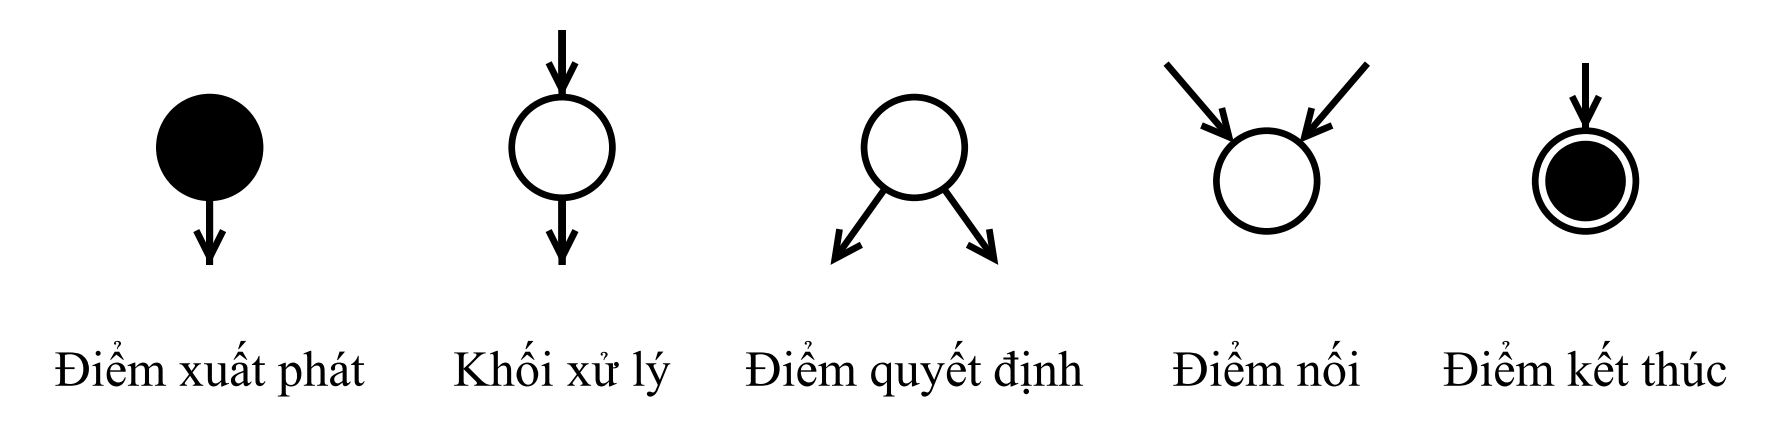
\includegraphics[width=\linewidth]{images/flow-element.png}
	\caption{Các thành phần cơ bản trong đồ thị dòng điều khiển.}
	\label{fig:flow-element}
\end{figure}

\begin{figure}[h]
	\centering
	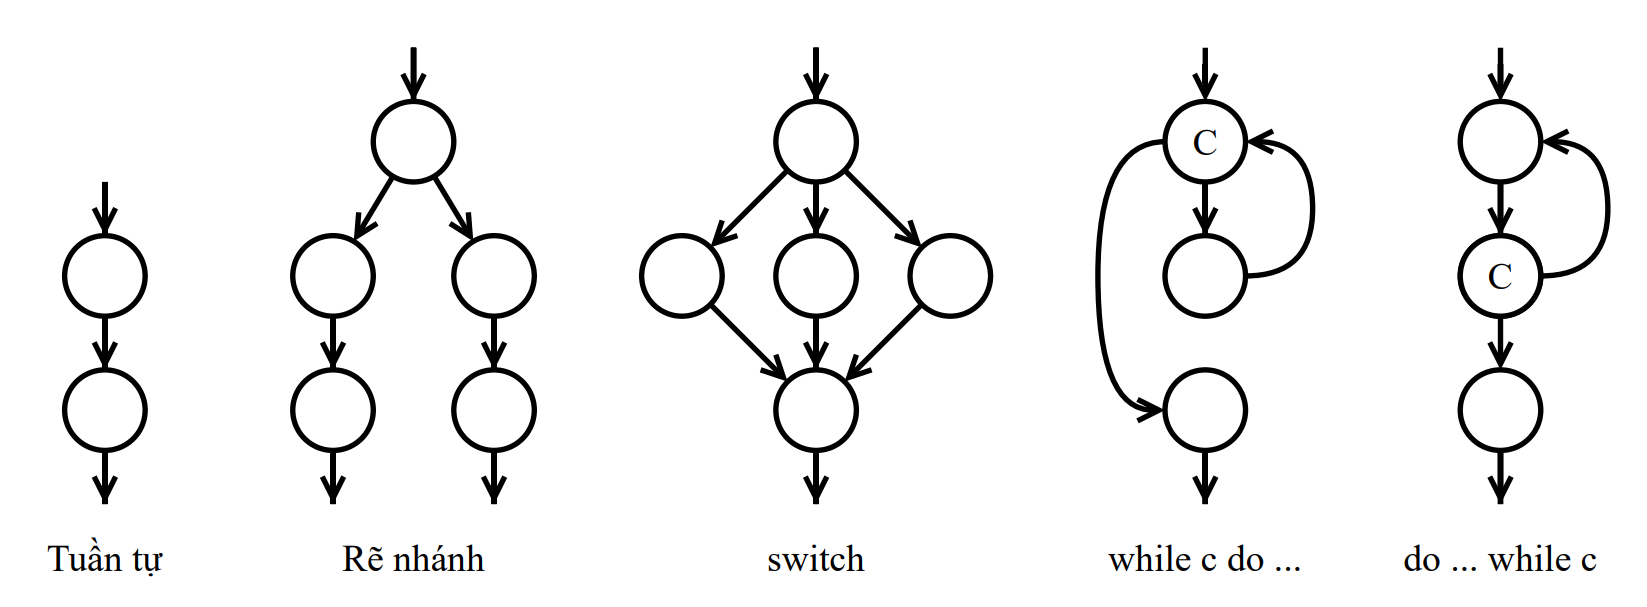
\includegraphics[width=\linewidth]{images/flow-structure.png}
	\caption{Các cấu trúc điều khiển phổ biến trong dồ thị dòng điều khiển.}
	\label{fig:flow-structure}
\end{figure}

\subsection{Đường thi hành}\label{sec:path}
Đường thi hành là một tập hợp có thứ tự các đỉnh trên CFG thể hiện thứ tự viếng thăm khi thực thi đơn vị kiểm thử tương ứng. Nói cách khác, đường thi hành biểu diễn các câu lệnh được chạy khi thực thi đơn vị kiểm thử với một bộ tham số đầu vào. Định nghĩa chính xác của đường thi hành như Định nghĩa 2.2.

\textbf{Định nghĩa 2.2}: Đường thi hành là một đường đi từ điểm xuất phát đến điểm kết thúc của CFG, được biểu diễn bằng tập hợp các điểm từ $v_1$ đến $v_n$ sao cho cứ hai điểm cạnh nhau thì có cạnh nối theo hướng từ trái qua phải. Nếu cạnh ($v_i$, $v_j$) là nhánh sai thì biểu thức điều kiện tại điểm $v_i$ được viết dưới dạng phủ định $!v_i$~\cite{GiaoTrinhKiemThu}.

Đường thi hành có thể chứa rất nhiều câu lệnh và rất nhiều nhánh điều kiện. Điều này dẫn tới việc một đơn vị kiểm thử có thể chứa đường thi hành không khả thi và có thể bùng nổ số lượng đường thi hành. Một đường thi hành không khả thi khi tồn tại những điều kiện không thể thỏa mãn được. Một ví dụ có thể kể đến đó là câu lệnh so sánh \tcode{if(0~==~1)}. Phép so sánh này không bao giờ đúng nên các đỉnh CFG trong nhánh đúng của đỉnh so sánh trên sẽ không thể viếng thăm. Về khả năng bùng nổ số lượng đường thi hành, điều này có thể thấy rõ thông qua các vòng lặp. Các vòng lặp với số lần lặp chưa biết trước có thể tạo ra vô số đường thi hành. Vì vậy việc kiểm thử toàn bộ đường thi hành là một thách thức lớn.

Như vậy, việc sinh dữ liệu kiểm thử cho một đường thi hành tương ứng với quá trình tìm giá trị bộ tham số đầu vào sao cho viếng thăm được toàn bộ đỉnh trên đường thi hành. Trong thực tế, số lượng đường thi hành của một đơn vị kiểm thử có thể rất lớn. Do vậy, việc lựa chọn tập đường thi hành sao cho đạt độ phủ mã nguồn yêu cầu là một thách thức lớn.

\subsection{Độ phủ mã nguồn} \label{sec:coverage}
Độ phủ mã nguồn là một đơn vị đo số lượng thành phần trong đơn vị kiểm thử được viếng thăm bởi bộ dữ liệu tham số đầu vào. Các thành phần liên quan có thể là câu lệnh, điểm quyết định, điều kiện con, đường thi hành hay là sự kết hợp của chúng \cite{GiaoTrinhKiemThu}. Bộ kiểm thử có độ tin cậy càng cao khi độ phủ đơn vị kiểm thử càng lớn. Ba loại độ phủ mã nguồn được sử dụng phổ biến trong thực tế gồm $C_1$, $C_2$ và $C_3$~\cite{GiaoTrinhKiemThu}. Một số tác giả sử dụng các khái niệm tương ứng gồm Statement, Branch và MCDC (Modified Condition/Decision Coverage). Khóa luận sử dụng khái niệm $C_1$, $C_2$ và $C_3$ với định nghĩa như sau:
\begin{itemize}
	\item Độ phủ $C_1$: Được hiểu là độ phủ ở mức câu lệnh, tức mỗi câu lệnh trong đơn vị kiểm thử được thực thi ít nhất một lần sau khi chạy tập ca kiểm thử.
	
	\item Độ phủ $C_2$: Được hiểu là độ phủ ở mức điểm quyết định, tức mỗi điểm quyết định trong CFG của đơn vị kiểm thử đều được thực hiện ít nhất một lần cả nhánh đúng và sai sau khi chạy tập ca kiểm thử.
	
	\item Độ phủ $C_3$: Là độ phủ có điều kiện chặt nhất trong ba loại độ phủ. Điều kiện để đảm bảo độ đo này là các điều kiện con thuộc các điều kiện phức tạp tương ứng với các điểm quyết định trong đồ thị dòng điều khiển của đơn vị cần kiểm thử đều được thực hiện ít nhất một lần cả hai nhánh đúng và sai. Với các phần mềm yêu cầu tính đúng đắn cao, việc sử dụng độ đo $C_3$ để đánh giá mã nguồn là cần thiết.
\end{itemize}

\section{Kiểm thử tượng trưng động}
Như đã đề cập ở Chương \nameref{chap1}, kiểm thử tượng trưng động là kĩ thuật kiểm thử áp dụng đồng thời kiểm thử tĩnh và kiểm thử động với ba pha chính là sinh dữ liệu kiểm thử ngẫu nhiên, thực thi ca kiểm thử \& phân tích đường thi hành và sinh dữ liệu kiểm thử có định hướng. Trong pha đầu tiên, một số dữ liệu kiểm thử được sinh ngẫu nhiên. Các dữ liệu kiểm thử sau đó được thực thi trong pha thứ hai. Nhờ việc thực thi các dữ liệu kiểm thử khởi tạo, kiểm thử tượng trưng động xác định được tập các điểm chưa được viếng thăm và
tìm kiếm đường thi hành từ điểm xuất phát đến điểm đó. Một số nhà nghiên cứu lựa chọn đường thi hành ngắn nhất tới một điểm chưa viếng thăm nhằm tối ưu hóa số lượng ca kiểm thử như SDART~\cite{SDART}. Nếu tìm được đường thi hành chưa được viếng thăm, pha thứ ba chuyển đổi đường thi hành thành các ràng buộc sử dụng kỹ thuật thực thi giá trị tượng trưng~\cite{SymbolicExecutionForSoftwareTestingThreeDecadesLater}. Các ràng buộc được biểu diễn dưới dạng biểu thức logic và được chuyển đổi thành đầu vào của bộ giải hệ ràng buộc. Cuối cùng, bộ giải hệ ràng buộc chịu trách nhiệm giải các ràng buộc và cho ra được một nghiệm - dữ liệu kiểm thử mới. Quá trình sinh dữ liệu kiểm thử sau đó lặp lại từ pha thứ hai cho đến khi tất cả đỉnh trong CFG đã được thăm hoặc chương trình chạy quá thời gian quy định. 

Kỹ thuật kiểm thử tượng trưng động có khả năng đạt độ phủ cao hơn bởi khả năng sinh dữ liệu có hướng dựa trên ràng buộc của đường thi hành. Tập ràng buộc là tập các điều kiện tạo ra bởi tập các kiểm quyết định khi áp dụng kỹ thuật thực thi tượng trưng trên một đường thi hành. Nói cách khác, tập ràng buộc chứa các điều kiện mà dữ liệu đầu vào cần thỏa mãn để ca kiểm thử phủ đường thi hành mong muốn. Dữ liệu đầu vào như vậy được gọi là dữ liệu kiểm thử có hướng. Dữ liệu kiểm thử có hướng cho mỗi đường thi hành có thể thu được bằng cách giải hệ ràng buộc. Trong đó, giải hệ ràng buộc là việc tìm nghiệm cho một tập các ràng buộc, biểu diễn bởi các phép toán điều kiện, sao cho với các giá trị biến đầu vào trong nghiệm thì tất cả các ràng buộc được thỏa mãn~\cite{ref-constraints}. Hiện nay, có nhiều thư viện và công cụ hỗ trợ giải hệ ràng buộc trong đó nổi bật là bộ giải Z3\footnote{https://github.com/Z3Prover/z3}.

Bộ giải Z3 là một công cụ được phát triển bởi Nhóm Nghiên cứu về Kỹ thuật Phần mềm (RiSE) tại Microsoft Research. Được xây dựng chủ yếu bằng ngôn ngữ C++, Z3 hỗ trợ giải hệ ràng buộc của nhiều loại dữ liệu như số nguyên, số thực, mảng, hàm tượng trưng, vectơ bit, và các biểu thức số học khác nhau. Z3 được thiết kế để hỗ trợ định dạng SMT-LIB\footnote{http://smtlib.github.io/jSMTLIB/SMTLIBTutorial.pdf}, một định dạng tiêu chuẩn sử dụng để giải quyết các vấn đề liên quan đến giải ràng buộc. Để sử dụng bộ giải, hệ ràng buộc cần được biểu diễn dưới định dạng SMT-LIB và lưu trữ trong tệp *.smt2. Cấu trúc của tệp này bao gồm ba phần chính: phần khai báo, phần định nghĩa ràng buộc và phần tiện ích. Phần khai báo đầu tiên trong tệp là nơi các biến trong hệ ràng buộc được khai báo theo cú pháp SMT-LIB. Sau đó, các ràng buộc được thêm vào bằng cách sử dụng lệnh assert. Cuối cùng, phần tiện ích cung cấp các cú pháp sẵn có để người dùng thực hiện các thao tác như đặt thời gian giải quyết tối đa, xác định mô hình giải ràng buộc, và nhiều tính năng khác.

\section{Hàm thiếu định nghĩa} \label{sec:kno-undefine}
\subsection{Tổng quan về hàm thiếu định nghĩa}
Như đã đề cập ở Chương~\nameref{chap1}, hàm thiếu định nghĩa là những hàm mà có nguyên mẫu được khai báo, nhưng không có thân hàm (định nghĩa hàm). Để làm rõ hơn khái niệm này, ta cần hiểu thêm về cách khai báo hàm trong ngôn ngữ C/C++. Về cơ bản, một hàm gồm hai phần chính đó là nguyên mẫu hàm và thân hàm. Trong đó, nguyên mẫu hàm thông báo cho trình biên dịch biết tên hàm, kiểu trả về của hàm và danh sách tham số mà hàm nhận. Thân hàm là phần nội dung của hàm nằm trong cặp ngoặc \tcode{\{\}}. Ngôn ngữ C/C++ cung cấp hai cách để người dùng khai báo một hàm (ngoại trừ hàm lambda) gồm khai báo đầy đủ và khai báo tách rời.
\vspace{5mm}
\begin{lstlisting}[language=C++, captionpos=b, caption={Ví dụ về khai báo hàm đầy đủ và khai báo hàm tách rời.}, label={cod:kno-undef}]
// Full function declaration
int foo(int a, int b) { return a + b; }
// Function prototype + Function defintion 
int bar(int a, int b);
int echo(double);
int main() { bar(1,2); }
int bar(int a, int b) { return a - b; }
\end{lstlisting}

Đoạn mã \ref{cod:kno-undef} minh họa ví dụ về khai báo đầy đủ và khai báo tách rời. Dòng~1-3 thể hiện khai báo tách rời của hàm~\tcode{foo} với nguyên mẫu hàm và thân hàm đều nằm trong cùng một câu lệnh khai báo. Dòng~6 thể hiện khai báo nguyên mẫu hàm của hàm~\tcode{bar} và cho biết hàm này trả về giá trị kiểu \tcode{int} và nhận hai tham số đầu vào kiểu \tcode{int}. Dòng~7 cũng thể hiện nguyên mẫu hàm \tcode{echo}. Dòng~11-13 thể hiện khai báo định nghĩa hàm (thân hàm) của hàm \tcode{bar}.

Nguyên mẫu hàm là một trong những tính năng quan trọng của ngôn ngữ C/C++. Nguyên mẫu hàm cung cấp cho trình biên dịch biết những thông tin cơ bản của hàm và trình biên dịch ngầm hiểu rằng định nghĩa của hàm này có tồn tại. Cơ chế này giúp tăng tính tái sử dụng mã nguồn trong ngôn ngữ C/C++ bởi người dùng có thể tái sử dụng các nguyên mẫu hàm trong tệp header mà không cần biết nội dung chi tiết trong hàm đó.

Nguyên mẫu hàm là một tính năng hữu ích song nó cũng có nhược điểm. Nhược điểm của tính năng này đó là sự phụ thuộc vào người dùng. Một nguyên mẫu hàm không cần thiết phải có định nghĩa hàm bởi có thể nó không được sử dụng trong mã nguồn. Với ví dụ trong Đoạn mã~\ref{cod:kno-undef}, nguyên mẫu hàm \tcode{echo} không cần có định nghĩa bởi nó không được sử dụng trong bất kì thành phần nào khác. Trình biên dịch có khả năng tự xác định các nguyên mẫu hàm được sử dụng khi phân tích cú pháp mã nguồn ở bước biên dịch. Quá trình liên kết các tệp đối tượng có mục đích xác định định nghĩa hàm tương ứng với từng nguyên mẫu hàm. Ở bước này, nếu trình biên dịch không thể tìm thấy định nghĩa hàm tương ứng, nguyên mẫu hàm được coi là hàm thiếu định nghĩa.
\subsection{Nguyên mẫu hàm ảo và lỗi thiếu bảng ký hiệu ảo}
Hàm ảo là một cơ chế mới được giới thiệu trong ngôn ngữ C++ nhằm thể hiện các đặc trưng hướng đối tượng so với ngôn ngữ C. Hàm ảo là một hàm đặc biệt, chỉ có thể khai báo trong lớp và có khả năng ghi đè bởi hàm ở lớp dẫn xuất. Khi hàm ảo ở lớp cơ sở được gọi, chương trình sẽ tự động hiểu và chọn đúng đối tượng ở lớp dẫn xuất để gọi đúng hàm ghi đè. Khả năng trên được gọi là đa hình. Nguyên mẫu hàm ảo cũng có các đặc điểm tương tự như nguyên mẫu hàm bình thường.

Để có được khả năng đa hình, ngôn ngữ C++ giới thiệu một khái niệm mới có tên là bảng ký hiệu ảo (Vtable). Vtable là bảng lưu trữ các khai báo biến, hàm có trong một kiểu dữ liệu tự định nghĩa do trình biên dịch tạo ra khi biên dịch một tệp mã nguồn. Vtable là công cụ giúp trình biên dịch biết một biến đã được định nghĩa hay chưa, biến đó thuộc kiểu gì, từ đó thông báo đến người dùng nếu có lỗi ngữ pháp. Vtable còn là công cụ giúp chương trình xác định được hàm nào sẽ được thực thi bằng cách sử dụng cơ chế liên kết động. Nếu hàm ảo, thuần ảo thiếu định nghĩa hàm thì khi liên kết, trình biên dịch sẽ báo lỗi do không biết chương trình sẽ cần hàm nào để chạy. Khác với các nguyên mẫu hàm bình thường, trình biên dịch không hiển thị lỗi hàm thiếu định nghĩa nếu không tìm thấy định nghĩa của hàm ảo mà sẽ hiển thị lỗi thiếu bảng ký hiệu ảo. Nguyên nhân gây ra lỗi này là bởi trình biên dịch không cho phép gọi hàm ảo nếu nó không có ít nhất một hàm ghi đè.\\

\begin{lstlisting}[language=C++, captionpos=b, caption={Ví dụ về lỗi thiếu bảng ký hiệu ảo.}, label={cod:kno-vtable}]
	class A {
		virtual int echo() {}
		virtual int foo();
		virtual int bar();
	};
	class B : public A {
		int bar() {}
	}
\end{lstlisting}

Để làm rõ hơn ví dụ về lỗi thiếu bảng ký hiệu ảo, ta xét ví dụ trong Đoạn mã~\ref{cod:kno-vtable}. Đoạn mã này chứa hai lớp \tcode{A} và \tcode{B} trong đó \tcode{B} là lớp dẫn xuất của \tcode{A}. Lớp \tcode{A} có chứa ba nguyên mẫu hàm ảo, trong đó hàm~\tcode{bar} được ghi đè ở lớp dẫn xuât và hàm~\tcode{echo} là khai báo hàm ảo đầy đủ. Trong quá trình liên kết để tạo thành tệp thực thi, trình biên dịch báo lỗi thiếu Vtable cho kiểu \tcode{A} bởi trình biên dịch không thể tìm thấy hàm ghi đè nguyên mẫu hàm ảo \tcode{foo} ở lớp dẫn xuất.

\subsection{Vai trò trong các dự án C/C++}
Kể từ khi được giới thiệu trong ngôn ngữ C, nguyên mẫu hàm đóng vai trò quan trọng các dự án C/C++ và được sử dụng phổ biến trong quá trình phát triển phần mềm.	Về mặt kỹ thuật, nguyên mẫu hàm giúp tạo ra một bản thiết kế cho các hàm trước khi chúng được triển khai. Điều này giúp kiểm soát việc sử dụng hàm, đồng thời cung cấp thông tin đầy đủ cho trình biên dịch để kiểm tra tính đúng đắn của mã nguồn. Về mặt phát triển, nguyên mẫu hàm cho phép các thành viên trong nhóm phát triển đặt ra những lớp giao diện, các hành vi sẽ được cung cấp bởi mô-đun họ phụ trách. Điều này thúc đẩy quá trình phát triển phần mềm nhanh hơn bởi các thành viên không cần phải đợi sự hoàn thiện từ các thành phần phụ thuộc. 

Trong ngôn ngữ C++, vai trò của nguyên mẫu hàm được bổ sung trong đặc trưng kế thừa và đa hình với nguyên mẫu hàm ảo. Khi một lớp cơ sở chứa một hàm ảo, các lớp kế thừa có thể cung cấp triển khai riêng của hàm đó mà không cần thay đổi nguyên mẫu. Điều này tạo điều kiện cho việc chia sẻ chức năng giữa các lớp và giúp tăng tính linh hoạt của hệ thống. Nguyên mẫu hàm ảo tạo ra khả năng đa hình, cho phép gọi hàm dựa trên kiểu đối tượng thực tế thay vì kiểu của biến con trỏ hay tham chiếu. Điều này làm cho mã nguồn trở nên linh hoạt và dễ bảo trì, đặc biệt là trong các hệ thống lớn với nhiều lớp và đối tượng.

Do quá trình kiểm thử đơn vị diễn ra song song với quá trình phát triển nên ta không thể tránh khỏi tình trạng mã nguồn tồn tại một số nguyên mẫu hàm thiếu định nghĩa. Vì vậy, nhu cầu phát triển một giải pháp kiểm thử tự động đặc biệt cho mã nguồn C/C++ chứa hàm thiếu định nghĩa là vô cùng thiết yếu. Theo khảo sát của khóa luận về phương pháp xử lý hàm thiếu định nghĩa, hiện chưa có phương pháp nào được đề xuất vậy nên khóa luận sẽ thảo luận chi tiết về phương pháp giải quyết ở Chương~\ref{chap3}.

\section{Sinh giả lập mã nguồn tự động} \label{sec:autostub-Lam}
Trong quá trình phát triển phần mềm, hai giai đoạn quan trọng là cài đặt và kiểm thử thường diễn ra đồng thời để giảm thiểu thời gian phát triển và đồng thời đảm bảo chất lượng sản phẩm. Tuy nhiên, điều này có thể dẫn đến việc mã nguồn kiểm thử chứa các thành phần chưa hoàn thiện. Điều này đặt ra thách thức khi đơn vị kiểm thử có thể chứa các lời gọi hàm chưa được đầy đủ, ảnh hưởng đến quá trình kiểm thử chính xác và hiệu quả.

Một số phương pháp sinh stub tự động đã được đề xuất để giải quyết bài toán trên. Trong đó, năm 2022, ông Trần Nguyên Hương và các cộng sự đã đề xuất phương pháp AS4UT~\cite{TUNG2022106821} giúp sinh stub tự động, sử dụng trong kiểm thử đơn vị các dự án C/C++. Ý tưởng chính của phương pháp là xem mỗi lời gọi hàm như một biến giả. Giai đoạn tiền xử lý CFG được thêm vào hướng tiếp cận kiểm thử tượng trưng động. Trong giai đoạn này, mọi lời gọi hàm trong CFG của đơn vị kiểm thử được thay thế bằng các biến giả tương ứng. CFG sau khi biến đổi được sử dụng làm đầu vào để thực hiện quá trình thực thi tượng trưng giúp tìm ra các bộ dữ liệu kiểm thử có hướng. Phương pháp AS4UT đem lại một số kết quả tích cực khi áp dụng vào một số dự án mã nguồn mở ngôn ngữ C với 87.88\% độ phủ $C_1$ trên dự án C-Algorithms\footnote{https://github.com/fragglet/c-algorithms}. Phương pháp này cũng cần ít hơn số ca kiểm thử để đạt được độ phủ cao hơn so với phương pháp kiểm thử tượng trưng động.

Phương pháp AS4UT khi áp dụng trên các dự án C++ bộc lộ một số hạn chế. Một trong số các hạn chế đó là việc xử lý lời gọi phương thức bởi phương pháp đang chú trọng vào kết quả trả về của lời gọi hàm mà chưa quan tâm tới các ảnh hưởng gây bởi lời gọi phương thức. Điều này có thể gây khó khăn khi kiểm thử các đơn vị có nhiều sự tương tác của các đội tượng bởi lời gọi phương thức có thể thay đổi gía trị thuộc tính của đối tượng.
\chapter{Phương pháp kiểm thử đơn vị tự động cho mã nguồn chứa hàm thiếu định nghĩa}
\section{Tổng quan phương pháp đề xuất}\label{sec:tongquan}
Về tổng quan, phương pháp đề xuất là sự kết hợp giữa phương pháp kiểm thử tượng trưng động~\cite{ConcolicTesting} và phương pháp sinh giả lập mã nguồn tự động~\cite{TUNG2022106821} với các cải tiến trong quá trình xử lý môi trường kiểm thử chứa hàm thiếu định nghĩa và quá trình thực thi tượng trưng lời gọi phương thức. Quá trình kiểm thử tự động bao gồm bốn pha được mô tả trong Hình~\ref{fig:proposed-flow}. Các pha được in đậm trong hình vẽ thể hiện chúng được bổ sung hoặc cải tiến bởi phương pháp đề xuất.

\begin{figure}[h]
    \centering
    \includesvg[width=\linewidth]{images/proposed-flow}
    \caption{Tổng quan phương pháp đề xuất.}
    \label{fig:proposed-flow}
\end{figure}

Pha đầu tiên trong phương pháp đề xuất là pha xây dựng môi trường kiểm thử. Hai nhiệm vụ chính của pha đó là thực hiện các tác vụ tiền xử lý trên mã nguồn kiểm thử và phân tích mã nguồn để xây dựng đồ thị cấu trúc mã nguồn kiểm thử. Nội dung chi tiết của pha xây dựng môi trường kiểm thử được trình bày trong Mục~\ref{sec:3-build-env}.

Pha tiếp theo trong phương pháp đề xuất là pha xử lý hàm thiếu nghĩa. Pha này được bổ sung so với phương pháp kiểm thử tự động truyền thống nhằm xử lý các vấn đề phát sinh bởi các hàm thiếu định nghĩa khi kiểm thử tự động cho các mã nguồn chưa hoàn chỉnh. Chi tiết về quá trình xử lý hàm thiếu định nghĩa được mô tả trong Mục~\ref{sec:handle-undef}.

Sau pha xử lý hàm thiếu định nghĩa, quá trình kiểm thử tự động chuyển sang pha sinh dữ liệu kiểm thử tự động cho các đơn vị kiểm thử. Khóa luận sử dụng phương pháp sinh kế thừa từ phương pháp sinh dữ liệu kiểm thử tượng trưng động và phương pháp sinh giả lập mã nguồn AS4UT (mô tả ở Mục~\ref{sec:autostub-Lam}). Trong pha sinh dữ liệu kiểm thử tự động, phương pháp đề xuất bổ sung bước sinh giả lập mã nguồn cho các hàm là phương thức của đối tượng nhằm tăng khả năng thực thi các câu lệnh, điều kiện có liên quan đến các đối tượng được sử dụng trong đơn vị kiểm thử. Nội dung chi tiết của pha sinh dữ liệu kiểm thử được trình bày ở Mục~\ref{sec:autogen}. 

Cuối cùng, các dữ liệu độ phủ được thu thập ở pha sinh dữ liệu kiểm thử được phân tích và tạo thành báo cáo kiểm thử trong pha sinh báo cáo độ phủ mã nguồn. Khóa luận sử dụng công cụ tính độ phủ GCOV và công cụ sinh báo cáo LCOV để thực hiện nhiệm vụ của pha. Trong đó, GCOV là công cụ phân tích độ phủ tích hợp sẵn trong gói của trình biên dịch C/C++ GNU, LCOV là một tiện ích mở rộng từ công cụ GCOV với nhiệm vụ sinh báo cáo độ phủ dạng HTML dựa trên các thông tin độ phủ của GCOV. GCOV và LCOV là hai công cụ có sẵn trong trình biên dịch và được sử dụng phổ biến trong các dự án~C/C++ \cite{hu2021software}. Quá trình thực thi ca kiểm thử ở pha trước sinh ra thông tin về số lần chạy qua một dòng, số lần chạy qua các nhánh điều kiện với từng trường hợp đúng, sai theo định dạng của GCOV. Thông tin này sau đó được LCOV tổng hợp, tính toán và đưa ra tệp báo cáo HTML.

\section{Pha xây dựng môi trường kiểm thử} \label{sec:3-build-env}
Như đã đề cập ở Mục \ref{sec:tongquan}, pha xây dựng môi trường kiểm thử thực hiện hai nhiệm vụ chính. Nhiệm vụ thứ nhất đó là thực hiện hai tác vụ tiền xử lý mã nguồn. Tác vụ đầu tiên là tác vụ thiết lập môi trường nhằm biên dịch mã nguồn và các ca kiểm thử về sau. Tác vụ này cài đặt các lệnh biên dịch, xác định và liên kết các thư viện mà mã nguồn sử dụng, thiết lập kiểu độ phủ mong muốn cho các đơn vị kiểm thử. Tác vụ thứ hai là tác vụ tạo môi trường tính toán độ phủ. Tác vụ này nhân bản mã nguồn kiểm thử và bổ sung các câu lệnh đánh dấu (instrumentation) nhằm phục vụ quá trình xác định các câu lệnh, nhánh được viếng thăm và tính toán độ phủ trong pha sinh dữ liệu kiểm thử tự động. Nhiệm vụ còn lại của pha đó là phân tích mã nguồn kiểm thử và xây dựng đồ thị cấu trúc mã nguồn. Bước phân tích mã nguồn sử dụng công cụ phân tích mã nguồn CDT Parser để trích xuất AST của mã nguồn kiểm thử. Từ thông tin trên AST, phương pháp đề xuất xây dựng đồ thị cấu trúc mã nguồn với các thông tin được phân tích đến mức hàm.

\subsection*{Đồ thị cấu trúc mã nguồn}
Đồ thị cấu trúc mã nguồn là một cấu trúc dữ liệu biểu diễn mối quan hệ và sự tương tác giữa các thành phần trong mã nguồn kiểm thử. Đồ thị này được biểu diễn bởi một đồ thị có hướng $G = (V, E)$, trong đó $V$ là tập các đỉnh tượng trưng cho các thành phần trong các đơn vị kiểm thử và $E$ là tập các cạnh có hướng nối giữa hai đỉnh tượng trưng cho mối quan hệ phát sinh giữa đỉnh đầu và đỉnh cuối. Mỗi đỉnh trong đồ thị biểu thị cho các đơn vị cơ bản như như tệp mã nguồn, lớp, biến, thư viện được sử dụng, các hàm, v.v. Để làm rõ thể hiện của các hàm thiếu định nghĩa trong đồ thị, khóa luận biểu thị hàm thành hai loại đỉnh hàm: đỉnh nguyên mẫu hàm và đỉnh định nghĩa hàm. Mỗi cạnh trong mã nguồn thuộc một trong các cạnh được mô tả dưới đây.
\begin{itemize}
    \item Cạnh cha con: Thể hiện mối quan hệ cha - con (hay mối quan hệ chứa) giữa hai đơn vị cơ bản trong đơn vị kiểm thử. Ví dụ cho mối quan hệ này có thể kể đến như lớp chứa một số thuộc tính và phương thức, tương đương quan hệ lớp là cha của các thuộc tính và phương thức.
    \item Cạnh Include: Thể hiện mối quan hệ Include giữa hai tệp mã nguồn. Ví dụ cho quan hệ này là dòng lệnh \tcode{\#include} thường thấy trong các mã nguồn C/C++.
    \item Cạnh kế thừa: Thể hiện mối quan hệ kế thừa giữa lớp cha và lớp dẫn xuất. Hai đỉnh của cạnh là hai đỉnh lớp.
    \item Cạnh lời gọi hàm: Thể hiện tương tác giữa hai hàm trong mã nguồn kiểm thử. Hai đỉnh của cạnh là hai đỉnh hàm. Cạnh lời gọi hàm là thành phần quan trọng trong bước xác định các hàm cần tạo stub khi kiểm thử tự động cho một hầm bất kì.
    \item Cạnh định nghĩa: Thể hiện mối quan hệ định nghĩa giữa đỉnh nguyên mẫu hàm ảo và đỉnh định nghĩa hàm ảo. Quan hệ định nghĩa thể hiện nguyên mẫu hàm được trỏ tới tồn tại một khai báo định nghĩa.
\end{itemize}

Đồ thị cấu trúc mã nguồn được xây dựng bằng việc mở rộng từng đỉnh tệp với các cạnh cha con. Quá trình mở rộng đỉnh tệp cấu thành một cây cấu trúc tệp. Tiếp theo, dựa trên các cây cấu trúc tệp, đồ thị cấu trúc mã nguồn được hoàn thiện bằng cách phân tích AST kết hợp tìm kiếm để bổ sung các cạnh quan hệ còn lại. Cạnh định nghĩa là trường hợp đặc biệt được bổ sung sau vào đồ thị trong pha xử lý hàm thiếu định nghĩa.

\subsection*{Ví dụ về đồ thị cấu trúc mã nguồn}
\begin{figure}[ht]
    \begin{minipage}[t]{0.5\linewidth}
    \begin{lstlisting}[language=C++, caption={Mã nguồn tệp \textit{a.cpp} minh họa đồ thị cấu trúc mã nguồn.}, label={cod:dep-cpp}, captionpos=b]
// a.cpp
#include "a.hpp"
int A::func() {
    /* Function logic */
}
double foo() {
    /* Some logic */
    int ret = stub();
    / * Some logic */
}
int stub() {
    /* Function logic */
}
    \end{lstlisting}
    \end{minipage}
    \begin{minipage}[t]{0.5\linewidth}
    \begin{lstlisting}[language=C++, caption={Mã nguồn tệp \textit{a.hpp} minh họa đồ thị cấu trúc mã nguồn.}, label={cod:dep-hpp}, captionpos=b]
// a.hpp
class IA {
public: 
    int bar();
};
class A : public IA {
public:
    A() {}
    int x;
    virtual int beta();
    virtual int func();
    double foo();
}; 
    \end{lstlisting}
\end{minipage}
\end{figure}

Hình \ref{fig:dep-graph} minh hoạ đồ thị cấu trúc mã nguồn của hai tệp mã nguồn a.hpp và a.cpp trong Đoạn mã \ref{cod:dep-cpp} và \ref{cod:dep-hpp}. Trong đó, các cạnh nét liền mũi tên đen thể hiện cạnh cha con giữa hai đỉnh và các kiểu cạnh còn lại được ký hiệu trên hình vẽ với thể hiện tương ứng. Cây cấu trúc mã nguồn của tệp \textit{a.cpp} gồm ba đỉnh hàm. Cây cấu trúc mã nguồn của tệp \textit{a.hpp} gồm hai đỉnh lớp, mỗi đỉnh lớp có quan hệ cha con với một số đỉnh như đỉnh thuộc tính, đỉnh nguyễn mẫu hàm. Cạnh Include từ đỉnh tệp \textit{a.cpp} tới đỉnh \textit{a.hpp} tương đương dòng lệnh \tcode{\#include "a.hpp"} trong Đoạn mã \ref{cod:dep-cpp}. Cạnh lời gọi hàm từ đỉnh định nghĩa hàm \tcode{double A::foo()} tới đỉnh định nghĩa hàm \tcode{int stub()} tương đương lời gọi hàm ở dòng 8 trong tệp \textit{a.cpp}. Đoạn mã ví dụ cho thấy nguyên mẫu hàm ảo \tcode{int func()} trong lớp A có tồn tại định nghĩa bởi hàm \tcode{int A::func()} nhưng đồ thị thiếu cạnh định nghĩa về quan hệ này do cạnh định nghĩa giữa hai đỉnh sẽ được bổ sung sau pha xử lý hàm thiếu định nghĩa.  
 
\begin{figure}[t]
    \centering
    \includesvg[width=\linewidth]{images/dep-graph}
    \caption{Ví dụ minh hoạ về đồ thị cấu trúc mã nguồn xây dựng trên mã nguồn tệp \textit{a.hpp} và \textit{a.cpp}.}
    \label{fig:dep-graph}
\end{figure}

\section{Pha xử lý hàm thiếu định nghĩa} \label{sec:handle-undef}
Pha xử lý hàm thiếu định nghĩa được bổ sung với hai nhiệm vụ chính đó là xử lý các nguyên mẫu hàm thiếu định nghĩa tìm được bởi trình biên dịch và xử lý các nguyên mẫu hàm ảo thiếu định nghĩa mà trình biên dịch không thể phát hiện được. Ý tưởng chung để giải quyết hai nhiệm vụ vừa đề cập dựa trên việc tìm kiếm các ứng viên nguyên mẫu hàm tương thích trong mã nguồn kiểm thử theo các tiêu chí thích hợp, sau đó sinh thân hàm giả cho các ứng viên này. Mục \ref{sec:handle-undef-first} mô tả cụ thể về phương pháp xử lý nhiệm vụ thứ nhất. Phương pháp xử lý nguyên mẫu hàm ảo được trình bày trong Mục \ref{sec:handle-undef-second}.

\subsection{ Phương pháp xử lý nguyên mẫu hàm thiếu định nghĩa tìm bởi trình biên dịch} \label{sec:handle-undef-first}
Khóa luận đề xuất phương pháp sử dụng trình biên dịch để tìm kiếm các nguyên mẫu hàm cần sinh thân hàm giả trong mã nguồn kiểm thử. Thuật toán \ref{alg:handle-ref} mô tả chi tiết quá trình tìm kiếm và xử lý các nguyên mẫu hàm thiếu định nghĩa. Trước hết, thuật toán bắt đầu bằng việc thu thập danh sách các nguyên mẫu hàm cần quan tâm trong tập các tệp mã nguồn $S$ và khởi tạo tập $T$ rỗng. Danh sách trả về bao gồm các xâu ký tự, mỗi xâu biểu thị một hàm bao gồm tên hàm và danh sách tham số của hàm đó (dòng~1-2). Tập $T$ là tập hợp các nguyên mẫu hàm trong mã nguồn kiểm thử được sinh thân hàm giả. Sau khi có danh sách, thuật toán xử lý từng xâu trong danh sách đầu vào (dòng~3-14). Cụ thể, với mỗi xâu, một AST $undef\_ast$ được xây dựng từ chữ ký hàm mà xâu biểu thị (dòng~4). Tiếp đó, tên của nguyên mẫu hàm được trích xuất từ AST vừa xây dựng (dòng~5) và tập các nguyên mẫu hàm ứng viên có cùng tên trong mã nguồn kiểm thử được thu thập và lưu vào danh sách $candidates$ (dòng~6). Danh sách tham số của nguyên mẫu hàm $undef$ và phạm vi định danh (scope qualifier) được trích xuất từ AST phục vụ cho quá trình lọc (dòng~7-8). Danh sách ứng viên được lọc bởi Thuật toán \ref{alg:filter-undef} và thu được các ứng viên hợp lệ $qualified\_cans$ (dòng~9). Cuối cùng, từng ứng viên hợp lệ $qc$ được sinh thân hàm giả và thêm vào tập $T$ (dòng~11-12). Dữ liệu trong tập $T$ được lưu lại để xây dựng môi trường kiểm thử cho mã nguồn đang xét trong các lần sau mà không cần xử lý lại từ đầu.

\begin{algorithm}[ht]
    \small
    \caption{Thuật toán xử lý hàm thiếu định nghĩa}
    \label{alg:handle-ref}
    \SetKwComment{Comment}{/* }{ */} 
    \KwIn{~$S$ - collection of source code files}
    \KwOut{~$T$ - collection of handled undefined functions}
					
    $undefined\_functions \leftarrow $ Get necessary undefined functions in $S$\;
    $T \leftarrow \emptyset$\;
    \For {$undef : undefined\_functions$} {
        $undef\_ast\leftarrow$ Construct AST from the string $undef$\;
        $undef\_name \leftarrow$ Get the name of the function from string $undef\_ast$\;
        $candidates \leftarrow$ Find all function prototypes having the same name with $undef\_name$ in source code\;
        $undef\_params \leftarrow$ Extract a list of parameters from $undef\_ast$\;
        $undef\_scope\leftarrow$ Extract function scope qualifier from $undef\_ast$\;
        $qualified\_cans\leftarrow$ \textbf{call} Algorithm \ref{alg:filter-undef} $(undef\_params, undef\_scope, candidates)$\;
        \For {$qc : qualified\_cans$} {
            $t \leftarrow $ Generate simple function body for $qc$\;
            $T \leftarrow T \cup {t}$
        }
    }

    \Return $T$
\end{algorithm}

\subsubsection*{Thu thập danh sách nguyên mẫu hàm thiếu định nghĩa}\label{sec:find-undef}
Ý tưởng sử dụng các công cụ tiện ích của trình biên dịch để tìm nguyên mẫu hàm cần quan tâm xuất phát từ lợi thế trình biên dịch biết hàm nào sẽ được sử dụng trong các tệp đối tượng như đã trình bày ở Mục \ref{sec:kno-undefine}. Đoạn mã \ref{cod:command-undef} mô tả cách dùng các công cụ tiện ích có trong trình biên dịch để tìm các nguyên mẫu hàm thiếu định nghĩa. Đầu tiên, phương pháp đề xuất sử dụng công cụ \textit{g++} với cờ \textit{-c} để biên dịch các tệp mã nguồn thành tệp đối tượng (object file) có đuôi \textit{.o} (dòng 1). Sau đó, các tệp đối tượng này sẽ được liên kết bởi công cụ liên kết \textit{ld} và cờ \textit{-r} thành một tệp đối tượng tổng hợp \textit{temp.o} (dòng 2). Lí do phương pháp đề xuất sử dụng công cụ liên kết \textit{ld} thay vì \textit{g++} là bởi \textit{g++} yêu cầu người dùng phải hoàn thiện tất cả các nguyên mẫu hàm bị thiếu định nghĩa trước khi liên kết thành tệp tổng hợp. Cuối cùng, tệp đối tượng tổng hợp được phân tích bởi công cụ phân tích ký hiệu \textit{nm}\footnote{https://sourceware.org/binutils/docs/binutils/nm.html} với các cờ \textit{-u} - trích xuất các hàm thiếu định nghĩa, \textit{-C} - chuyển ký hiệu máy thành ngôn ngữ lập trình C++ (dòng 3). Đầu ra của công cụ \textit{nm} sẽ được ghi vào tệp \textit{list.txt}.\\

\begin{lstlisting}[language=C++, caption={Các câu lệnh tìm nguyên mẫu hàm thiếu định nghĩa cần quan tâm sử dụng trình biên dịch.}, label={cod:command-undef},  captionpos=b]
g++ -c *.cpp
ld -r *.o -o temp.o
nm temp.o -u -C > list.txt
\end{lstlisting}

\begin{figure}[t]
    \begin{minipage}[t]{0.5\linewidth}
    \begin{lstlisting}[language=C++, caption={Mã nguồn tệp a.cpp.}, label={cod:undef-cpp}, captionpos=b]
// a.cpp
#include "a.hpp"
#include "b.hpp"
    
int foo(A *a, int x) {
    int ret = a->bar(true);
    int max = maxT<int>(x, ret);
    max += a->echo();
    const int *p = &(a->x);
    ret -= func(p, max);
    return ret;
}

void gamma(A *a, int x) {
    double max = maxT<double>(x, a->x);
    a->x = max;
}
int unused(int x);
    \end{lstlisting}
    \end{minipage}
    \begin{minipage}[t]{0.5\linewidth}
    \begin{lstlisting}[language=C++, caption={Mã nguồn tệp a.hpp, b.hpp và c.hpp.}, label={cod:undef-hpp}, captionpos=b]
// a.hpp
#include "c.hpp"
class A {
public: 
    int x;
    A(int _x) { x = _x; }
    int bar(bool b);
    double echo() {
        return x + delta(&x);
    }
};
int bar(bool b);
// b.hpp
template <typename T> T max(T a);
int func(int *a, int b);
int func(const int* a, int b);
    
// c.hpp
double delta(int* const x);  
    \end{lstlisting}
\end{minipage}
\end{figure}

Đoạn mã \ref{cod:undef-cpp} và \ref{cod:undef-hpp} minh họa cách áp dụng phương pháp đề xuất trên tập đơn vị kiểm thử cần xử lý các nguyên mẫu hàm thiếu định nghĩa với bốn tệp mã nguồn. Kiểm thử viên muốn kiểm thử tự động cho hai hàm có lôgic đầy đủ \tcode{foo} và \tcode{gamma}. Hai hàm này chứa mã nguồn đầy đủ. Hai đoạn mã chứa một số nguyên mẫu hàm đó là \tcode{unused}, \tcode{bar}, \tcode{delta} và ba hàm trong tệp \tcode{b.hpp}.Hàm \tcode{foo} trong Đoạn mã \ref{cod:undef-cpp} nhận đầu vào là một biến con trỏ đến đối tượng của lớp \tcode{A} và một biến kiểu nguyên \tcode{x}. Lôgic mã nguồn của \tcode{foo} gọi tới hai phương thức của biến \tcode{a} đó là \tcode{bar} và \tcode{echo}. Ngoài ra, hàm \tcode{foo} còn gọi tới nguyên mẫu hàm template \tcode{maxT} với kiểu khởi tạo \tcode{int} và hàm \tcode{func(const int* a, int b)} thuộc tệp \tcode{b.hpp}. Hàm \tcode{gamma} cũng có các đầu vào tương tự nhưng gọi nguyên mẫu hàm \tcode{maxT} nhưng sử dụng tham số kiểu \tcode{double} thay vì \tcode{int} như hàm \tcode{foo}.

Đoạn mã \ref{cod:result-undef} minh họa danh sách các nguyên mẫu hàm cần quan tâm trong tệp các đơn vị kiểm thử \textit{a.cpp}, \textit{a.hpp}, \textit{b.hpp} và \textit{c.hpp} khi áp dụng phương pháp đề xuất. Dòng đầu tiên cho biết nguyên mẫu hàm \tcode{func(int const*, int)} cần được xử lý, tương đương với hàm \tcode{func(const int* a, int b)} trong mã nguồn \textit{b.hpp} (dòng 16 trong Đoạn~mã~\ref{cod:undef-hpp}). Dòng 2 và 3 biểu thị cú pháp của hàm template. Đối với trình biên dịch, các lời gọi hàm template với các kiểu đối số khác nhau sẽ tạo ra các chữ ký hàm khác nhau. Do hàm \tcode{foo} và \tcode{gamma} gọi hàm \tcode{maxT} với hai đối số kiểu khác nhau nên danh sách các nguyên mẫu hàm thiếu định nghĩa chứa chữ ký hàm cho cả hai kiểu này. Tiếp theo, nguyên mẫu hàm ở dòng 4 tương ứng hàm \tcode{delta(int* const x)} trong tệp c.hpp. Tham số hiển thị ở tệp mã nguồn và trên danh sách khác nhau là bởi trình biên dịch chỉ quan tâm tới kiểu của tham số và loại bỏ lớp lưu trữ (storage class) ngoài cùng của tham số đó. Tham số \tcode{x} của hàm \tcode{delta} có kiểu là \tcode{int* const} tức con trỏ hằng trỏ tới một biến kiểu nguyên. Trình biên dịch chuyển kiểu của tham số trên thành \tcode{int*}. Trong trường hợp của hai hàm \tcode{func}, tham số đầu của hai hàm khác nhau là bởi tham số \tcode{const int* a} được trình biên dịch chuyển thành kiểu \tcode{const int*} do từ khoá \tcode{const} là lớp lưu trữ của biến được tham số trỏ tới. Cuối cùng nguyên mẫu hàm \tcode{A::bar(bool)} tương ứng với nguyên mẫu hàm \tcode{int bar(bool b)} trong lớp \tcode{A} (dòng 7 trong Đoạn mã \ref{cod:undef-hpp}).
\begin{figure}[t]
\begin{lstlisting}[language=C++, caption={Danh sách các nguyên mẫu hàm thiếu định nghĩa tìm bởi trình biên dịch.}, label={cod:result-undef}, captionpos=b]
func(int const*, int)
double maxT<double>(double, double)        
int maxT<int>(int, int)     
delta(int*)
A::bar(bool)         
\end{lstlisting}
\end{figure}
\subsubsection*{Lọc tìm ứng viên hợp lệ}
Như đã mô tả trong ví dụ minh hoạ ở Đoạn mã \ref{cod:result-undef}, mỗi nguyên mẫu hàm trong danh sách trả về bởi trình biên dịch sẽ tương ứng với một số nguyên mẫu hàm trong mã nguồn gốc. Để ánh xạ từng nguyên mẫu hàm cần quan tâm tới đúng nguyên mẫu hàm trong đơn vị kiểm thử, phương pháp đề xuất sử dụng ba tiêu chí để đánh giá độ phù hợp của từng ứng viên. Tiêu chí đầu tiên đó là hàm ứng viên chưa được ánh xạ bởi bất kỳ nguyên mẫu hàm nào trên danh sách. Tiêu chí thứ hai đó là số lượng tham số và phạm vi định danh của hai hàm phải giống nhau. Tiêu chí này giúp giảm số lượng các ứng viên có cùng tên cần xét. Cuối cùng, ứng viên hợp lệ nếu từng tham số đã chuẩn hoá của ứng viên có cùng kiểu với tham số tương ứng của nguyên mẫu hàm.
\begin{algorithm}
    \small
    \caption{Thuật toán lọc tìm ứng viên hợp lệ}
    \label{alg:filter-undef}
    \SetKwComment{Comment}{/* }{ */} 
    \KwIn{~$undef\_params$ - list of parameters extracted from the string $undef$ \\
    \hskip 1.1cm $undef\_scope$ - the scope qualifier of $undef$\\
    \hskip 1.1cm  $candidates$ - list of function prototypes having the same name
    }
    \KwOut{~$qualified\_cans$ - list of qualified function prototypes}
					
    $qualified\_cans \leftarrow$ Initial empty list\;
    \For {$candidate : candidates$} {
        \uIf {$candidate$ \textbf{is} \textit{handled}} {
            \textbf{continue}
        }
        \Else {
            $can\_params \leftarrow$ Extract a list of parameters of function $candidate$\;
            $can\_scope\leftarrow$ Get the scope qualifier of $candidate$\;
            \uIf {$can\_params.length \neq undef\_params.length$ \textbf{or} $can\_scope \neq undef\_scope$} {
                \textbf{continue}
            }
            \Else {
                $same\_params \leftarrow$ \textbf{True}\;
                $iter\leftarrow$ 1 \Comment*[r]{Assume the list starts at index 1}
                \While{$iter \leq can\_params.length$} {
                    $can\_param\_iter\leftarrow$ Normalize the $iter^{th}$ param of $can\_params$\;
                    $undef\_param\leftarrow$ Get the $iter^{th}$ param of $under\_params$ \;
                    \uIf{$can\_param\_iter$ \textbf{has the same type with} $under\_params$} {
                        $iter++$
                    }
                    \Else {
                        $same\_params\leftarrow$ \textbf{False}\;
                        \textbf{break}
                    }
                }

                \If{$same\_params\leftarrow$ \textbf{True}} {
                    Set $candidate$ state to $handled$\;
                    Push $candidate$ into $qualified\_cans$\;
                }
            }
        }
    }
    \KwRet{$qualified\_cans$}
\end{algorithm}

Thuật toán \ref{alg:filter-undef} mô tả chi tiết cách áp dụng ba tiêu chí để lọc ra các ứng viên hợp lệ. Đầu vào của thuật toán gồm danh sách tham số trích xuất từ nguyên mẫu hàm cần tìm và danh sách nguyên mẫu hàm ứng viên trong mã nguồn kiểm thử. Mỗi ứng viên sẽ được xét duyệt lần lượt trên ba tiêu chí (dòng 3-28). Nếu ứng viên $candidate$ đã được ánh xạ (hay có trạng thái $handled$), ứng viên sẽ được bỏ qua (dòng 3-4). Ngược lại, danh sách tham số của ứng viên $candidate$ được trích xuất để sử dụng cho hai tiêu chí còn lại (dòng~6). Nếu số lượng tham số hoặc phạm vi định danh của ứng viên khác nguyên mẫu hàm đầu vào thì ứng viên này sẽ được bỏ qua (dòng~8-9). Để áp dụng tiêu chí thứ ba một cách hiệu quả, phương pháp đề xuất xét duyệt lần lượt từng tham số và dừng lại khi gặp tham số đầu tiên không hợp lệ. Trước hết, thuật toán khởi tạo biến $same\_params$ dùng để đánh dấu tất cả tham số đều hợp lệ và gán biến $iter$ bằng vị trí đầu tiên trong danh sách tham số (dòng~11-12). Tiếp đó, quá trình lặp đánh giá từng tham số diễn ra cho đến hết danh sách tham số hoặc gặp tham số không hợp lệ (dòng~13-22). Tham số thứ $iter$ của ứng viên và hàm đầu vào được lấy ra (dòng~13-14). Do tham số của hàm đầu vào đã được chuẩn hoá theo tiêu chuẩn của C++\footnote{https://www.open-std.org/jtc1/sc22/wg21/docs/standards}\footnote{https://en.cppreference.com/w/cpp/language/function} nên tham số của ứng viên cũng sẽ được đưa về theo các tiêu chuẩn này. Nếu hai tham số đang xét có cùng kiểu thì thuật toán sẽ chuyển sang tham số tiếp theo (dòng 16-17). Ngược lại, quá trình lặp sẽ kết thúc và thuật toán đánh dấu tính hợp lệ là $False$ (dòng 19-20). Sau quá trình đánh giá, nếu tất cả tham số của ứng viên đều hợp lệ, thuật toán chuyển trạng thái của ứng viên thành đã được ánh xạ và thêm vào danh sách ứng viên hợp lệ.

\subsubsection*{Ví dụ về xử lý nguyên mẫu hàm thiếu định nghĩa}
Để làm rõ hơn cách hoạt động của Thuật toán \ref{alg:filter-undef}, ta xét ví dụ áp dụng Thuật toán \ref{alg:handle-ref} trên danh sách các hàm trả về ở Đoạn mã \ref{cod:result-undef}. Xét ví dụ áp dụng phương pháp đề xuất trên xâu ký tự \textit{func(int const*, int)} (dòng 1), trước hết AST của nguyên mẫu hàm được xây dựng như Hình \ref{fig:func-ast}. AST gồm hai thành phần chính: tên của hàm (nút trái) và danh sách tham số (nút phải). Dựa vào thông tin trên cây AST, thuật toán trích xuất được tên \tcode{func} và danh sách tham số \tcode{{int const*, int}} và phạm vi định danh là không gian tên toàn cục. Tiếp theo thuật toán thu thập danh sách các nguyên mẫu hàm ứng viên có cùng tên \tcode{func} trong mã nguồn kiểm thử. Từ Đoạn mã \ref{cod:undef-hpp}, thuật toán thu được hai hàm \tcode{func(int *a, int b)} và \tcode{func(const int* a, int b)} (dòng 15-16). Sau đó, phương pháp đề xuất áp dụng Thuật toán \ref{alg:filter-undef} với hai ứng viên cùng các thông tin trích xuất được. Bảng \ref{tab:filter-func} minh hoạ cho quá trình lọc hai ứng viên. Các ứng viên được xét lần lượt theo thứ tự xuất hiện từ trên xuống của bảng. Với mỗi ứng viên, thuật toán lọc trên từng tiêu chí được liệt kê theo thứ tự từ trên xuống và thuật toán dừng khi tất cả tiêu chí đều hợp lệ hoặc gặp tiêu chí đầu tiên không hợp lệ. Bảng minh hoạ cho thấy ứng viên \tcode{func(int* a, int b)} không hợp lệ do kiểu của tham số đầu tiên sau khi chuẩn hoá là \tcode{int*}, không phải \tcode{int const*}. Ứng viên \tcode{func(const int* a, int b)} đều hợp lệ trên tất cả các tiêu chí nên nguyên mẫu hàm này sẽ được sinh thân hàm giả. \\
\begin{figure}[h]
    \centering
    \includesvg[width=\linewidth]{images/func-ast}
    \caption{AST (bên trái) và các thông tin trích xuất được (bên phải) của nguyên mẫu hàm \tcode{func(int const*, int}) trong Đoạn mã \ref{cod:result-undef}.}
    \label{fig:func-ast}
\end{figure}

\begin{table}[h]
\centering
\caption{Bảng minh hoạ tính hợp lệ của hai ứng viên cùng tên \tcode{func} trên từng tiêu chí}
\label{tab:filter-func}
\begin{tabular}{|l|ll|l|}
\hline
\textbf{Ứng viên}                          & \multicolumn{2}{l|}{\textbf{Tiêu chí}}                                                            & \textbf{Hợp lệ} \\ \hline
\multirow{3}{*}{\tcode{func(int* a, int b)}}       & \multicolumn{2}{l|}{Chưa có ánh xạ}                                                               & Có              \\ \cline{2-4} 
                                           & \multicolumn{2}{l|}{\begin{tabular}[c]{@{}l@{}}Số lượng tham số\\ Phạm vi định danh\end{tabular}} & Có              \\ \cline{2-4} 
                                           & \multicolumn{1}{l|}{Danh sách kiểu tham số}                              & int*                   & Không           \\ \hline
\multirow{4}{*}{\tcode{func(const int* a, int b)}} & \multicolumn{2}{l|}{Chưa có ánh xạ}                                                               & Có              \\ \cline{2-4} 
                                           & \multicolumn{2}{l|}{\begin{tabular}[c]{@{}l@{}}Số lượng tham số\\ Phạm vi định danh\end{tabular}} & Có              \\ \cline{2-4} 
                                           & \multicolumn{1}{l|}{\multirow{2}{*}{Danh sách kiểu tham số}}             & int const*             & Có              \\ \cline{3-4} 
                                           & \multicolumn{1}{l|}{}                                                    & int                    & Có              \\ \hline
\end{tabular}
\end{table}

\begin{figure}[h]
    \centering
    \includesvg[width=\linewidth]{images/bar-ast}
    \caption{AST (bên trái) và các thông tin trích xuất được (bên phải) của nguyên mẫu hàm \tcode{A::bar(bool)} trong Đoạn mã \ref{cod:result-undef}.}
    \label{fig:bar-ast}
\end{figure}

Khi xét áp dụng thuật toán với xâu \tcode{func(int const*, int)}, phương pháp đề xuất chưa bộc lộ khả năng giảm số lượng ứng viên cần xét của tiêu chí thứ hai. Nhằm làm rõ khả năng này, ta xét ví dụ áp dụng thuật toán với xâu \tcode{A::bar(bool)}. Tương tự như với xâu \tcode{func(int const*, int)}, trước hết, AST và các thông tin của nguyên mẫu hàm được trích xuất như Hình \ref{fig:bar-ast}. Phạm vi định danh của nguyên mẫu hàm đang xét không phải không gian tên toàn cục mà thuộc về không gian tên của lớp \tcode{A}. Các ứng viên có cùng tên \tcode{bar} trong mã nguồn kiểm thử bao gồm hàm \tcode{A::bar(bool~b)} và \tcode{bar(bool~b)}. Dựa các thông tin trích xuất được, quá trình lọc ứng viên áp dụng Thuật~toán~\ref{alg:filter-undef} và được minh hoạ qua Bảng \ref{tab:filter-bar}. Như vậy, khi xét ứng viên \tcode{bar(bool~b)}, Thuật~toán~\ref{alg:filter-undef} không cần xét tính hợp lệ của tiêu chí thứ ba mà vẫn loại bỏ được ứng viên. Điều này có thể lý giải bởi phạm vi định danh của ứng viên này là không gian tên toàn cục, không phải trong không tên của lớp \tcode{A}. Áp dụng thuật toán đề xuất trên các xâu còn lại trong danh sách, phương pháp đề xuất thu được mã nguồn kiểm thử đã bổ sung các thân hàm giả cần thiết như trong Đoạn mã \ref{cod:final-undef}. Từ danh sách các nguyên mẫu hàm cần quan tâm trả về bởi trình biên dịch, phương pháp đề xuất đã thêm thân hàm giả \tcode{\{/*~Insert~stub~code~later~*/\}} vào các nguyên mẫu hàm tương ứng trong mã nguồn kiểm thử. Các nguyên mẫu hàm này sau đó sẽ được thiết lập và sinh stub tự động trong quá trình sinh dữ liệu kiểm thử tự động.

% Please add the following required packages to your document preamble:
% \usepackage{multirow}
\begin{table}[h]
\centering
\caption{Bảng minh hoạ tính hợp lệ của hai ứng viên cùng tên \tcode{bar} trên từng tiêu chí}
\label{tab:filter-bar}
\begin{tabular}{|l|ll|l|}
\hline
\textbf{Ứng viên}                   & \multicolumn{2}{l|}{\textbf{Tiêu chí}}                                                            & \textbf{Hợp lệ} \\ \hline
\multirow{3}{*}{\tcode{int A::bar(bool b)}} & \multicolumn{2}{l|}{Chưa có ánh xạ}                                                               & Có              \\ \cline{2-4} 
                                    & \multicolumn{2}{l|}{\begin{tabular}[c]{@{}l@{}}Số lượng tham số\\ Phạm vi định danh\end{tabular}} & Có              \\ \cline{2-4} 
                                    & \multicolumn{1}{l|}{Danh sách kiểu tham số}                         & bool                        & Có              \\ \hline
\multirow{2}{*}{int bar(bool b)}    & \multicolumn{2}{l|}{Chưa có ánh xạ}                                                               & Có              \\ \cline{2-4} 
                                    & \multicolumn{2}{l|}{\begin{tabular}[c]{@{}l@{}}Số lượng tham số\\ Phạm vi định danh\end{tabular}} & Không           \\ \hline
\end{tabular}
\end{table}

\begin{figure}[ht]
    \centering
    \begin{lstlisting}[language=C++, caption={Mã nguồn tệp a.hpp, b.hpp và c.hpp sau khi áp dụng phương pháp xử lý nguyên mẫu hàm thiếu định nghĩa.}, label={cod:final-undef}, captionpos=b]
// a.hpp
#include "c.hpp"
class A {
public: 
    int x;
    A(int _x) { x = _x; }
    int bar(bool b) {/* Insert stub code later */ }
    double echo() {
        return x + delta(&x);
    }
};
int bar(bool b);
// b.hpp
template <typename T> T max(T a) {/* Insert stub code later */ }
int func(int *a, int b);
int func(const int* a, int b) {/* Insert stub code later */ }
// c.hpp
double delta(int* const x) {/* Insert stub code later */ }
    \end{lstlisting}
\end{figure}

% \begin{figure}
%     \begin{subfigure}[b]{.45\linewidth}
%         \includesvg[width=\linewidth]{images/bar-ast}
%         \caption{A gull}\label{fig:gull}
%     \end{subfigure}
%     \begin{subfigure}[b]{.45\linewidth}
%         \includesvg[width=\linewidth]{images/maxT-ast}
%         \caption{A tiger}\label{fig:tiger}
%     \end{subfigure}
% \caption{Picture of animals}
% \label{fig:animals}
% \end{figure}

\subsection{Phương pháp xử lý nguyên mẫu hàm ảo thiếu định nghĩa} \label{sec:handle-undef-second}
Như đã đề cập ở Mục \ref{sec:kno-undefine}, các hàm thiếu định nghĩa không chỉ gây lỗi thiếu tham chiếu khi liên kết các tệp đối tượng mà còn gây ra lỗi thiếu bảng hàm ảo. Điều này cũng đồng nghĩa với việc các nguyên mẫu hàm ảo thiếu định nghĩa, nguyên nhân gây ra lỗi, không thể tìm thấy bởi phương pháp đề xuất ở Mục \ref{sec:handle-undef-first} do quá trình liên kết các tệp đối tượng chỉ cho biết lớp đối tượng nào đang thiếu bảng hàm ảo mà không chỉ rõ rằng do nguyên mẫu hàm ảo nào gây ra. Phương pháp đề xuất giải quyết vấn đề này dựa trên việc xét duyệt các đỉnh nguyên mẫu hàm ảo trên từng cây cấu trúc tệp và tìm kiếm sự tồn tại của cạnh quan hệ định nghĩa trỏ tới đỉnh này trong đồ thị cấu trúc mã nguồn. Nếu đỉnh nguyên mẫu hàm ảo không tồn tại cạnh định nghĩa thì phương pháp đề xuất sẽ sinh thân hàm giả cho hàm này.

\subsection*{Thuật toán xử lý nguyên mẫu hàm ảo thiếu định nghĩa}

\begin{algorithm}[t]
    \small
    \caption{Thuật toán xử lý nguyên mẫu hàm ảo thiếu định nghĩa}
    \label{alg:handle-virtual-undef}
    \KwIn{~$project\_graph$ - the project structure graph}
    \KwOut{~$project\_graph$ - the modified graph with new definition edges}
    \For {$file\_tree : project\_graph$} {
        $cur\_file\_node \leftarrow $ Get file node of $file\_tree$\;
        $T \leftarrow {file\_tree}$\;
        $T \leftarrow T \cup$ {Get all file struct tree of file nodes that include $cur\_file\_node$}\;
        \For{$undef\_virtual : file\_tree$} {
            $undef\_name \leftarrow$ Get the name of the function from $undef\_virtual$\;
            $candidates \leftarrow$ Find all definition functions having the same name with $undef\_name$ in $T$\;
            $undef\_params \leftarrow$ Extract a list of parameters from $undef\_virtual$\;
            $undef\_scope\leftarrow$ Extract function scope qualifier from $undef\_virtual$\;
            $qualified\_cans\leftarrow$ \textbf{call} Algorithm \ref{alg:filter-undef} $(undef\_params, undef\_scope, candidates)$\;
            \uIf{$qualified\_cans = \emptyset$} {
                Generate a simple function body for $undef\_virtual$\;
            }
            \Else{
                $qc \leftarrow $ Get the first qualified candidate\;
                Generate definition edge for $qc$ and $undef\_virtual$ on $project\_graph$\;
            }
        }
    }
    \KwRet{$project\_graph$}
\end{algorithm}

Phương pháp xử lý nguyên mẫu hàm ảo thiếu định nghĩa được mô tả chi tiết trong Thuật toán \ref{alg:handle-virtual-undef}. Đầu vào của thuật toán là đồ thị cấu trúc mã nguồn được xây dựng ở pha xây dựng môi trường kiểm thử. Thuật toán xét duyệt từng cây cấu trúc tệp $file\_tree$ trong đồ thị đầu vào. Với mỗi cây cấu trúc $file\_tree$, trước hết, thuật toán thu thập tập hợp $T$ các cây cấu trúc có đỉnh tệp có cạnh Include tới đỉnh tệp của $file\_tree$ (dòng~2-4). Bản thân $file\_tree$ cũng được thêm vào tập hợp này để xét trường hợp định nghĩa của nguyên mẫu hàm ảo được khai báo ngay trong chính cây cấu trúc chứa nguyên mẫu. Tiếp theo, thuật toán xét duyệt từng đỉnh nguyên mẫu hàm ảo có trong cây cấu trúc tệp $file\_tree$. Với mỗi đỉnh nguyên mẫu hàm ảo, thuật toán trích xuất các thông tin như tên (dòng 6), danh sách tham số (dòng 8) và phạm vi định danh (dòng 9). Danh sách các đỉnh định nghĩa hàm ứng viên có cùng tên được thu thập (dòng 7). Sau đó, thuật toán áp dụng phương pháp lọc tìm kiếm ứng viên phù hợp trong Thuật toán \ref{alg:filter-undef} để lấy danh sách ứng viên hợp lệ (dòng 10). Nếu danh sách ứng viên hợp lệ rỗng tức nguyên mẫu hàm ảo không có định nghĩa hàm tương ứng thì thuật toán sẽ sinh thân hàm giả cho hàm này (dòng 11-12). Ngược lại, do đỉnh định nghĩa hàm luôn là duy nhất nên thuật toán sinh cạnh định nghĩa giữa ứng viên hợp lệ duy nhất và đỉnh nguyên mẫu hàm ảo đang xét (dòng 14-15). Thuật toán diễn ra tương tự với các đỉnh nguyên mẫu hàm ảo còn lại và tương tự với các cây cấu trúc tệp khác. Đầu ra của thuật toán là đồ thị cấu trúc mã nguồn với các cạnh bổ sung. Đồ thị đầu ra sẽ được lưu lại để phục vụ cho các lần kiểm thử sau trên mã nguồn đang xét.

\subsection*{Ví dụ về xử lý nguyên mẫu hàm ảo thiếu định nghĩa}
Đoạn mã \ref{cod:dep-cpp} và \ref{cod:dep-hpp} trong ví dụ minh họa độ thị cấu trúc mã nguồn chứa hai nguyên mẫu hàm ảo \tcode{beta()} và \tcode{func()}. Trong đó hàm \tcode{beta()} là nguyên mẫu hàm ảo thiếu định nghĩa. Để minh họa phương pháp đề xuất, ta xét ví dụ áp dụng Thuật toán \ref{alg:handle-virtual-undef} để xử lý hai nguyên mẫu hàm ảo trên. Trước hết, thuật toán xét cây cấu trúc tệp có đỉnh tệp \textit{a.hpp} (gọi tắt là cây cấu trúc \textit{a.hpp}) và thu thập tập hợp $T$ chứa các cây cấu trúc tệp có đỉnh tệp có cạnh Include tới đỉnh tệp \textit{a.hpp}. Dựa trên đồ thị cấu trúc mã nguồn như Hình~\ref{fig:dep-graph}, tập $T$ thu được gồm hai cây cấu trúc: cây gốc đang xét \textit{a.hpp} và cây cấu trúc \textit{a.cpp}. Tiếp theo, thuật toán xét từng nguyên mẫu hàm ảo có trong cây cấu trúc \textit{a.hpp}. Đối với hàm \tcode{func()}, thuật toán trích xuất các thông tin của hàm và thu được như sau: tên hàm là \tcode{func}, hàm không có tham số và phạm vi định danh là lớp \tcode{A}. Dựa trên thông tin này, thuật toán tìm các ứng viên có cùng tên \tcode{func} và thu được đỉnh định nghĩa hàm \tcode{A::func()}. Do ứng viên này hợp lệ trên cả ba tiêu chí của Thuật toán \ref{alg:filter-undef} nên ứng viên này là định nghĩa hàm của nguyên mẫu hàm \tcode{func()}. Do có tồn tại một ứng viên hợp lệ nên thuật toán sinh cạnh định nghĩa giữa đỉnh ứng viên và đỉnh nguyên mẫu hàm \tcode{func()}. Đối với hàm \tcode{beta()}, các bước tương tự được áp dụng. Tuy nhiên, do không tồn tại ứng viên có cùng tên \tcode{beta} nên nguyên mẫu hàm ảo này được xác định là thiếu định nghĩa. Do vậy, thuật toán sinh thân hàm giả cho hàm này theo quy tắc của phương pháp xử lý nguyên mẫu hàm thiếu định nghĩa ở Mục \ref{sec:handle-undef-first} Thuật toán tiếp tục xử lý tương tự với cây cấu trúc \textit{a.cpp}. Hình \ref{fig:dep-graph-final} mô tả sự thay đổi của đồ thị cấu trúc mã nguồn sau quá trình xử lý. Cạnh đậm, nét đứt, đầu hình tròn thể hiện cạnh định nghĩa được bổ sung sau quá trình.

\begin{figure}[!h]
    \centering
    \includesvg[width=\linewidth]{images/dep-graph-final}
    \caption{Ví dụ minh hoạ sự thay đổi đồ thị cấu trúc mã nguồn \textit{a.hpp} và \textit{a.cpp} sau khi xử lý hàm thiếu định nghĩa.}
    \label{fig:dep-graph-final}
\end{figure}

\section{Pha sinh dữ liệu kiểm thử tự động} \label{sec:autogen}
Trong các dự án thực tế, mỗi hàm cần kiểm thử có thể chứa rất nhiều lời gọi tới các hàm khác trong mã nguồn kiểm thử. Do các dự án hiện nay thường phát triển song song với kiểm thử đảm bảo chất lượng nên mã nguồn có thể chứa nhiều hàm chưa được hoàn thiện logic hoặc mới chỉ có nguyên mẫu hàm. Khóa luận đã đề xuất phương pháp để giải quyết các nguyên mẫu hàm thiếu định nghĩa song vẫn cần giải quyết bài toán sinh dữ liệu kiểm thử tự động một cách hiệu quả cho các mã nguồn chưa hoàn thiện. Do vậy, khóa luận đề xuất phương pháp sinh dữ liệu kiểm thử tự động áp dụng phương pháp kiểm thử tượng trưng động \cite{DART, CUTE, TUNG2022106821} và phương pháp sinh giả lập mã nguồn (stub) tự động AS4UT \cite{9953784} để xử lý bài toán vừa đề cập. Với các dự án hướng đối tượng C++, các biến được sử dụng trong hàm có thể xoay quanh các đối tượng. Các đối tượng có thể chứa các phương thức chưa được hoàn thiện, chỉ có nguyên mẫu hàm để thông báo cho đội phát triển biết đối tượng này có thể làm gì. Như vậy, luồng logic trong hàm có thể ảnh hưởng lớn bởi các phương thức của đối tượng. Do phương pháp sinh stub tự động chưa xử lý được các trường hợp liên quan đến phương thức của đối tượng nên khóa luận bổ sung cải tiến để xử lý vấn đề trên.

\subsection{Tổng quan pha sinh dữ liệu kiểm thử tự động}

\begin{figure}[hb]
    \centering
    \includesvg[width=\linewidth]{images/autogen-flow}
    \caption{Tổng quan quá trình sinh dữ liệu kiểm thử tự động.}
    \label{fig:autogen-flow}
\end{figure}

Về tổng quan, quá trình sinh dữ liệu kiểm thử tự động bao gồm ba bước như trong Hình \ref{fig:autogen-flow}. Các bước trong phương pháp đề xuất được kế thừa từ phương pháp sinh dữ liệu kiểm thử tự động cho con trỏ void và con trỏ hàm VFP \cite{TUNG2022106821}. Trong đó, bước sinh dữ liệu kiểm thử có hướng được bổ sung phương pháp sinh stub tự động AS4UT và phương pháp xử lý lời gọi phương thức của đối tượng do khóa luận đề xuất. Bước đầu tiên trong quá trình là bước sinh dữ liệu kiểm thử ngẫu nhiên. Nhiệm vụ của bước này là phân tích kiểu dữ liệu của các tham số được sử dụng trong hàm đang kiểm thử. Các tham số này là tham số đầu vào của hàm, biến toàn cục và một đối tượng giả để gọi hàm nếu hàm đang kiểm thử là một phương thức trong lớp. Bước sinh dữ liệu ngẫu nhiên sẽ sinh giá trị ngẫu nhiên trong khoảng giá trị cho phép của kiểu dữ liệu cho từng tham số. Trong bước này, giá trị trả về của các lời gọi hàm cũng được sinh ngẫu nhiên. Tập hợp giá trị của tập tham số sẽ tạo thành các bộ dữ liệu kiểm thử. Bước tiếp theo là bước thực thi dữ liệu kiểm thử và phân tích đường thi hành. Bước này có hai nhiệm vụ chính. Nhiệm vụ thứ nhất đó là thực thi các bộ dữ liệu kiểm thử tạo ra bởi bước sinh dữ liệu kiểm thử ngẫu nhiên hoặc bước sinh dữ liệu kiểm thử có hướng. Đầu ra của việc thực thi dữ liệu kiểm thử là tập đường thi hành được viếng thăm bởi các bộ dữ liệu kiểm thử. Nhiệm vụ thứ hai của bước này đó là phân tích đường thi hành nhằm tìm ra đường thi hành ngắn nhất tới câu lệnh hoặc điều kiện chưa được viếng thăm. Nếu tồn tại đường thi hành chưa được viếng thăm, bước bốn sinh dữ liệu kiểm thử có hướng và tạo stub tự động được thực hiện. Nhiệm vụ của bước bốn là sinh dữ liệu kiểm thử tự động sao cho thăm được các câu lệnh hoặc điều kiện chưa được thăm. Phương pháp AS4UT \cite{9953784} được tích hợp trong quá trình thực thi tượng trưng nhằm xử lý các lời gọi hàm trong đơn vị kiểm thử. Cụ thể, khóa luận áp dụng bước tiền xử lý CFG trong phương pháp AS4UT trong quá trình thực thi tượng trưng trên một đường thi hành. Khóa luận cải tiến bước tiền xử lý CFG này và bổ sung bước xử lý lời gọi phương thức. Chi tiết về phương pháp xử lý lời gọi phương thức được trình bày ở Mục \ref{sec:autostub-obj} Đầu ra của bước này là tập các ràng buộc trên đường thi hành đang xét. Sau đó, phương pháp đề xuất sử dụng bộ giải hệ Z3 để tìm nghiệm cho các ràng buộc và chuyển nghiệm thành dữ liệu kiểm thử mới. Các dữ liệu kiểm thử mới này tiếp tục được thực thi và phân tích đường thi hành đầu ra. Quá trình sinh dữ liệu kiểm thử tự động được lặp lại cho đến khi không thể tìm thấy đường thi hành chưa thử viếng thăm.

\subsection{Phương pháp xử lý lời gọi phương thức của đối tượng} \label{sec:autostub-obj}
Như đã đề cập ở trên, phương thức của đối tượng có ảnh hưởng lớn tới hàm đang kiểm thử bởi thuộc tính của đối tượng có thể thay đổi qua các phương thức này. Khi đó, sau lời gọi phương thức, các biểu thức điều kiện sử dụng thuộc tính phụ thuộc nhiều vào sự thay đổi bởi lời gọi phương thức. Để thăm được các điều kiện chưa thăm được do có sự thay đổi bởi lời gọi phương thức, quá trình tiền xử lý CFG cần chú trọng xử lý các lời gọi này. Khóa luận đề xuất Thuật toán \ref{alg:autostub-object} để xử lý lời gọi phương thức. Ý tưởng chính của thuật toán đề xuất đó là bổ sung một đối tượng giả kèm theo giá trị trả về khi xuất hiện lời gọi phương thức và cập nhật biến thực thi tượng trưng của đối tượng gọi phương thức bằng đối tượng giả. 

Thuận toán \ref{alg:autostub-object} có bốn đầu vào lần lượt là bảng băm $MAP$, bảng tham chiếu $REF$, câu lệnh xuất lệnh lời gọi hàm $stm$ và đỉnh CFG $cfg\_node$ tương ứng với câu lệnh đang xét. Bảng băm $MAP$ là bảng băm ánh xạ các hàm sang số lần gọi của hàm đó trong đơn vị kiểm thử. Bảng tham chiếu $REF$ là bảng lưu trữ ánh xạ giữa biến tượng trưng và giá trị tượng trưng tương ứng của nó. Bảng $MAP$ và $REF$ được phương pháp đề xuất kế thừa từ phương pháp AS4UT. Đỉnh CFG đầu vào được lấy từ CFG gốc của đơn vị kiểm thử. Thuật toán bắt đầu với việc trích xuất hàm được gọi $function$ từ đỉnh CFG đầu vào (dòng 1) và khởi tạo số lần gọi hiện tại của hàm đó là 0 (dòng 2). Nếu hàm $function$ đã tồn tại trong $MAP$ thì thuật toán cập nhật số lần gọi hiện tại bằng số lần gọi cuối của $function$ trong $MAP$ (dòng 3-5). Tiếp theo, thuật toán tăng số lần gọi hiện tại $cur\_call$ lên 1 (dòng 6) và thêm cặp ánh xạ $(function, cur\_call)$ vào $MAP$ (dòng 7). Giá trị cũ nếu có của $function$ trong $MAP$ sẽ được thay bởi cặp ánh xạ mới này. Thuật toán trích xuất tên $func\_name$ và kiểu trả về $return\_type$ của $function$ (dòng 8) và xác định đối tượng gọi hàm $function$ (dòng 9). Nếu đối tượng trả về khác $NULL$ (hay hàm đang xét là phương thức) thuật toán sẽ tạo đối tượng giả trả về (dòng 11-16). Trước hết, tên $object\_name$ và kiểu $object\_type$ của đối tượng được trích xuất (dòng 11). Sau đó, thuật toán tạo tên đối tượng giả $stub\_name$ (dòng 12) và khởi tạo đối tượng giả với tên vừa tạo và kiểu đã xác định (dòng 13). Tiếp theo, thuật toán tìm kiếm biến tượng trưng $ref\_object$ có cùng tên và kiểu của đối tượng gốc (dòng 14). Đối tượng giả sẽ được đánh dấu trỏ tới biến tượng trưng $ref\_object$ (dòng 15) và được thêm vào $REF$ (dòng 16). Việc đánh dấu đối tượng giả trỏ tới biến tượng trưng của đối tượng gốc có nghĩa là đối tượng giả này sẽ được sử dụng thay cho biến tượng trưng trong các câu lệnh sau của đơn vị kiểm thử. Bước sinh biến tượng trưng cho giá trị trả về (dòng 18-23) được kế thừa từ phương pháp AS4UT. Trước hết, thuật toán sinh biến tượng trưng cho giá trị trả về của hàm (dòng 19-20). Sau đó, biến tượng trưng này được thêm vào bảng $REF$ (dòng 21) và thuật toán thay lời gọi hàm trong $stm$ bằng biến tượng trưng vừa tạo. Cuối cùng, thuật toán trả về bảng $MAP$, $REF$ và câu lệnh đã được cập nhật. Các thành phần sẽ tiếp tục được sử dụng bởi quá trình thực thi tượng trưng.  

\begin{algorithm}[!h]
    \small
    \caption{Thuật toán xử lý lời gọi phương thức của đối tượng}
    \label{alg:autostub-object}
    \KwIn{~$MAP$ - the map table transforming a function to its number of call\\
    \hskip 1.2cm $REF$ - the reference table containing symbolic variables\\
    \hskip 1.2cm $stm$ - the statement containing the function call expression \\
    \hskip 1.2cm $cfg\_node$ - the corresponding CFG node of current $stm$
    }
    \KwOut{~$MAP$ - the updated map table \\
    \hskip 1.2cm $REF$ - the updated reference table \\
    \hskip 1.2cm $stm$ - the refactored statement
    }
    $function \leftarrow$ Get the called function from $cfg\_node$\;
    $cur\_call \leftarrow 0$\;
    \If{$function \in MAP$} {
        $cur\_call \leftarrow $ Get the number of call of $function$ from $MAP$\; 
    }
    $cur\_call++$\;
    Insert $(function, cur\_call)$ into $MAP$\;
    $(func\_name, return\_type) \leftarrow$ Get the name and return type of $function$\;
    $call\_object \leftarrow$ Get the object calling the $function$\;
    \If{$call\_object \neq NULL$} {
        $(object\_name, object\_type) \leftarrow$ Get the name and type of $call\_object$\;
        $stub\_name \leftarrow func\_name + "\_call" + cur\_call + "\_" + object\_name$\;
        $instance\_stub\_var \leftarrow$ Generate new instance symbolic variable $(stub\_name, object\_type)$\;
        $ref\_object \leftarrow$ Get the class/struct symbolic variable having the same $(object\_name, object\_type)$ from $REF$\;
        Mark $instance\_stub\_var$ pointing to $ref\_object$\;
        Add $instance\_stub\_var$ into $REF$\;
    }
    \If{$return\_type$ \textbf{is not} void} {
        $stub\_name \leftarrow func\_name + "\_call" + cur\_call$\;
        $return\_stub\_var \leftarrow$ Generate return symbolic variable $(stub\_name, return\_type)$\;
        Add $return\_stub\_var$ into $REF$\;
        $stm \leftarrow$ Replace function call expression by $stub\_name$\;
    }
    \KwRet{$(MAP, REF, stm)$}
\end{algorithm}

\subsection{Ví dụ về thực thi tượng trưng kết hợp xử lý lời gọi phương thức của đối tượng}
Đoạn mã \ref{cod:autostub-object} mô tả đoạn mã nguồn ví dụ minh họa phương pháp tạo stub tự động cho phương thức của đối tượng. Đơn vị được kiểm thử là hàm \tcode{foo(B param)} với tham số đầu vào là \tcode{param}, một đối tượng của lớp \tcode{B}. Đồ thị dòng điều khiển của đơn vị này được mô tả trong Hình \ref{fig:cfg-object}. Logic của đơn vị kiểm thử gồm hai câu lệnh điều kiện, một câu lệnh gọi hàm và một hai câu lệnh trả giá trị. Dựa trên đồ thị dòng điều khiển khi xét đường thi hành 8-9-10-11, ta có thể nhận thấy điều kiện \tcode{if (param.b == 2)} tại dòng 10 bị ảnh hưởng với câu lệnh gọi phương thức ở dòng số 9. Hình \ref{fig:autostub-sample} mô tả quá trình thực thi tượng trưng áp dụng phương pháp đề xuất trên đường thi hành 8-9-10-11. Hình vẽ có bốn cột lần lượt biểu diễn đỉnh CFG đang xét, dữ liệu trong bảng $MAP$ và bảng $REF$ sau bước thực thi tượng trưng tại đỉnh CFG và cuối cùng là ràng buộc mới được sinh ra. Đầu tiên, ở trạng thái khởi tạo, quá trình thực thi tượng trưng tạo các biến tượng trưng cho tham số của hàm. Hàm \tcode{foo(B param)} có một tham số đầu vào nên một biến tượng trưng \tcode{param} được tạo ra và có giá trị tượng trưng \tcode{sym\_param}. Khi xét đỉnh CFG của câu điều kiện \tcode{if (param.b == 1)}, dựa trên bảng $REF$ quá trình thực thi tượng trưng tạo ra ràng buộc mới \tcode{sym\_param.b == 1}. Xét tiếp đỉnh CFG của câu lệnh \tcode{int ret = param.stub()}, lúc này, Thuật toán \ref{alg:autostub-object} được áp dụng để xử lý lời gọi phương thức của đối tượng \tcode{param}. Trước hết thuật toán cập nhật số lần gọi hàm \tcode{stub} lên 1 và lưu vào bảng $MAP$. Do hàm \tcode{stub} là phương thức nên thuật toán sẽ sinh đối tượng giả kèm theo giá trị trả về cho hàm này. Ba biến tượng trưng mới được cập nhật trong bảng $REF$ gồm \tcode{stub\_call1} - giá trị trả về tượng trưng, \tcode{ret} - biến được gán giá trị trả về của phương thức và \tcode{stub\_call1\_param} - đối tượng giả trỏ tới biến tượng trưng \tcode{param}. Xét tiếp tới đỉnh CFG của câu điều kiện \tcode{if (param.b == 2)}, dựa trên thông tin của bảng $REF$, quá trình thực thi tượng trưng sẽ chuyển đổi biến \tcode{param} gốc thành \tcode{sym\_param} và từ \tcode{sym\_param} thành \tcode{stub\_call1\_param}. Như vậy một ràng buộc mới được sinh ra đó là \tcode{stub\_call1\_param.b == 2}. Ràng buộc này có thể hiểu là thông qua lời gọi phương thức \tcode{stub}, giá trị của thuộc tính \tcode{b} trong đối tượng \tcode{param} cần phải thay đổi thành 2 thay vì 1 như khởi tạo. Qua quá trình thực thi tượng trưng trên đường thi hành 8-9-10-11 kết hợp với bảng $MAP$ và $REF$, ta thu được ba ràng buộc {stub\_call == 1, sym\_param.b == 1, stub\_call1\_param.b == 2}. Các ràng buộc này sau đó được chuẩn hóa theo cú pháp của SMTLib (ví dụ như hay \tcode{.b} thành \tcode{\_attr\_b}) và được đưa vào bộ giải Z3 để tìm nghiệm. Từ nghiệm tìm được, ta xác định được bộ dữ liệu kiểm thử để đi được đường thi hành 8-9-10-11 đó là biến \tcode{param} đầu cần khởi tạo thuộc tính \tcode{b} với giá trị 1, hàm \tcode{stub} được gọi 1 lần và trả về giá trị bất kỳ đồng thời thay đổi giá trị của thuộc tính \tcode{b} thành 2. 
\begin{figure}[ht]
    \begin{tabular}{cc}
    \begin{minipage}[b]{0.5\textwidth}
    \begin{lstlisting}[language=C++, caption={Mã nguồn minh họa phương pháp tạo stub tự động cho phương thức của đối tượng.}, label={cod:autostub-object}, captionpos=b]
class B {
public:
    int b;
    B() {}
    int stub() {}
};
int foo(B param) {
    if (param.b == 1) {
        int ret = param.stub();
        if (param.b == 2) {
            return ret;
        }
    }
    return 0;
}
    \end{lstlisting}
    \end{minipage}
    & \begin{minipage}[b]{0.4\textwidth}
        \centering
        \includesvg[width=\linewidth]{images/cfg-object.svg}
        \caption{Đồ thị dòng điều khiển của hàm \tcode{foo(B param)} trong Đoạn mã \ref{cod:autostub-object}.}
        \label{fig:cfg-object}
    \end{minipage}
    \end{tabular}
\end{figure}
\begin{figure}[h]
    \centering
    \includesvg[width=\linewidth]{images/autostub-sample.svg}
    \caption{Quá trình thực thi tượng trưng kết hợp Thuật toán \ref{alg:autostub-object}.}
    \label{fig:autostub-sample}
\end{figure}
Đoạn mã \ref{cod:stub-final} mô tả nội dung của hàm \tcode{stub} với bộ dữ liệu kiểm thử mới. Biến tĩnh \tcode{cur\_call} lưu số lần gọi hàm trong một lần thực thi ca kiểm thử. Biến này được tăng lên một với mỗi lần gọi hàm. Câu lệnh điều kiện ở dòng 8 dùng để kiểm tra xem chương trình đang thực hiện kiểm thử cho hàm nào. Biến \tcode{TEST\_CASE\_NAME} là một xâu kí tự toàn cục tạo bởi trình điều khiển kiểm thử nhằm lưu tên hàm đang kiểm thử. Do ví dụ đang xét kiểm thử trên hàm \tcode{foo} nên giả lập mã nguồn của hàm \tcode{stub} sẽ nằm trong các dòng 9-14. Câu lệnh điều kiện \tcode{cur\_call == 1} thể hiện nếu đây là lần gọi thứ nhất của hàm \tcode{stub}, hàm này sẽ thực hiện các giả lập mã nguồn được viết trong nhánh đúng của điều kiện này. Dòng 10-13 của mã nguồn kiểm thử cho biết mã nguồn giả lập cho lần gọi thứ nhất thực hiện hai nhiệm vụ. Nhiệm vụ thứ nhất đó là thay đổi giá trị của thuộc tính \tcode{b} (dòng 11). Nhiệm vụ thứ hai đó là tạo giá trị trả về cho hàm. Do không có ràng buộc liên quan đến giá trị trả về của hàm \tcode{stub} nên phương pháp đề xuất chọn giá trị 0 để trả về.

\begin{figure}[h]
\begin{lstlisting}[language=C++, caption={Sự thay đổi của hàm \tcode{stub} với bộ dữ liệu kiểm thử mới.}, label={cod:stub-final}, captionpos=b]
class B {
public:
    int b;
    B() {}
    int stub() {
        static int cur_call = 0;
        cur_call++;
        if (TEST_CASE_NAME == "foo") {
            if (cur_call == 1) {
                int stub_call1_param_attr_b = 2;
                this->b = stub_call1_param_attr_b;
                int stub_call1 = 0;
                return stub_call1;
            }
        }
    }
};
int foo(B param) {
    if (param.b == 1) {
        int ret = param.stub();
        if (param.b == 2) {
            return ret;
        }
    }
    return 0;
}
    \end{lstlisting}
\end{figure}
\chapter{Cài đặt công cụ và thực nghiệm}\label{chap4}
\section{Công cụ thực nghiệm}
Nhằm đánh giá tính hiệu quả của phương pháp đề xuất, khóa luận đã cài đặt một số mô-đun và tích hợp phương pháp đề xuất trên công cụ AKAUTAUTO và thực hiện thực nghiệm trên công cụ này. AKAUTAUTO là một công cụ kiểm thử tự động cho mã nguồn C/C++, được nghiên cứu và phát triển bởi Phòng thí nghiệm Đảm bảo chất lượng phần mềm (Khoa Công nghệ thông tin, Trường Đại học Công nghệ, ĐHQGHN) và đơn vị FPT-GAM (FPT Global Automative \& Manufacturing). Khóa luận kế thừa kiến trúc của công cụ AKAUTAUTO phiên bản 5.9.2, phiên bản tích hợp sẵn phương pháp kiểm thử tượng trưng động và phương pháp sinh giả lập mã nguồn tự động AS4UT, và bổ sung, cải tiến một số mô-đun trong kiến trúc gốc để tích hợp phương pháp đề xuất (phiên bản 5.9.2-thesis).

\subsection{Tổng quan kiến trúc công cụ AKAUTAUTO}
Công cụ AKUTAUTO được phát triển bằng ngôn ngữ Java với kiến trúc bao gồm sáu mô-đun chính lần lượt là mô-đun xây dựng môi trường kiểm thử, mô-đun phân tích mã nguồn, mô-đun xử lý hàm thiếu định nghĩa, mô-đun sinh dữ liệu kiểm thử, mô-đun thực thi \& phân tích ca kiểm thử và mô-đun sinh báo cáo kiểm thử. Hình \ref{fig:architect} mô tả kiến trúc của công cụ AKAUTAUTO gồm sáu mô-đun kể trên và các thành phần ngoài gồm trình biên dịch C/C++, bộ giải Z3 và thư viện phân tích mã nguồn CDT Parser. Trong đó, khóa luận đã bổ sung mô-đun xử lý hàm thiếu định nghĩa so với kiến trúc gốc, và cải tiến hai mô-đun phân tích mã nguồn và mô-đun sinh dữ liệu kiểm thử (thể hiện bởi các khối in đậm).

\begin{figure}[t]
    \centering
    \includesvg[width=\linewidth]{images/architect.svg}
    \caption{Kiến trúc công cụ AKAUTAUTO.}
    \label{fig:architect}
\end{figure}

Đầu vào của công cụ AKAUTAUTO gồm hai thành phần chính lần lượt là các tệp mã nguồn kiểm thử và cấu hình kiểm thử. Hai thành phần này được cung cấp bởi kiểm thử viên hoặc lập trình viên. Mô-đun xây dựng môi trường kiểm thử là mô-đun tiếp nhận các thành phần đầu vào và đảm nhiệm vai trò thực hiện hai tác vụ tiền xử lý mã nguồn trong pha xây dựng môi trường kiểm thử. Hai tác vụ tiền xử lý đã được đề cập ở Mục~\ref{sec:3-build-env} gồm thiết lập môi trường và tạo môi trường tính toán độ phủ. Mô-đun xây dựng môi trường kiểm thử cấu thành bởi ba thành phần chính đó là thành phần thiết lập môi trường, thành phần tải dự án và thành phần tạo môi trường tính toán độ phủ. Trong đó, hai thành phần thiết lập môi trường và tạo môi trường tính toán độ phủ thực hiện hai tác vụ tương ứng đã nêu. Thành phần tải dự án có nhiệm vụ xác định các tệp mã nguồn được người dùng thiết lập, sau đó kiến tạo đỉnh tệp của từng cây cấu trúc tệp tương ứng. Đầu ra của mô-đun gồm các tệp mã nguồn đã được thêm lệnh đánh dấu và tập các cây cấu trúc tệp cơ bản sinh bởi thành phần tải dự án. Các tệp mã nguồn chứa lệnh đánh dấu sẽ được sử dụng bởi mô-đun xử lý hàm thiếu định nghĩa nhằm sinh thân hàm giả trên tệp mã nguồn này. Tập cây cấu trúc tệp cơ bản và mã nguồn gốc sẽ được phân tích bởi mô-đun phân tích mã nguồn.

Các mô-đun tiếp theo trong kiến trúc của công cụ AKAUTAUTO được khóa luận bổ sung hoặc cải tiến gồm mô-đun phân tích mã nguồn, mô-đun xử lý hàm thiếu định nghĩa và mô-đun sinh dữ liệu kiểm thử. Chi tiết về sự cải tiến của mô-đun phân tích mã nguồn và mô-đun sinh dữ liệu kiểm thử được trình bày lần lượt ở Mục~\ref{sec:module-analyze} và Mục~\ref{sec:module-autogen}. Mô-đun xử lý hàm thiếu định nghĩa được bổ sung so với kiến trúc gốc nhằm giải quyết các vấn đề phát sinh bởi nguyên mẫu hàm thiếu định nghĩa. Nội dung chi tiết của mô-đun này được trình bày ở Mục~\ref{sec:module-undef}. 

Khóa luận kế thừa mô-đun thực thi và phân tích ca kiểm thử từ kiến trúc gốc của công cụ. Mô-đun này đóng vai trò  sinh trình điều khiển kiểm thử, thực thi trình điều khiển và phân tích đường thi hành thu được sau khi chạy ca kiểm thử. Cấu trúc của mô-đun gồm ba thành phần chính với nhiệm vụ chi tiết của từng thành phần như sau:
\begin{itemize}
    \item Thành phần sinh trình điều khiển kiểm thử: Đảm nhiệm hai vai trò chuyển đổi bộ nghiệm giải từ ràng buộc thành dữ liệu kiểm thử C++ và sinh trình điều khiển kiểm thử dựa trên dữ liệu mới. Trình điều khiển kiểm thử là một tệp C++ được tự động sinh ra nhằm chuyển đổi dữ liệu kiểm thử C++ thành các cú pháp C++ giúp khởi tạo giá trị tham số đầu vào của đơn vị kiểm thử. Các cú pháp C++ trong trình điều khiển gồm hai phần chính đó là phần định nghĩa tham số đầu vào và phần gọi đơn vị kiểm thử. Trình điều khiển cũng đảm nhiệm chuyển hóa dữ liệu kiểm thử C++ thành các mã nguồn giả lập cho các hàm cần stub.
    \item Thành phần thực thi ca kiểm thử: Có nhiệm vụ biên dịch trình điều khiển và các tệp mã nguồn chứa lệnh đánh dấu thành tệp đối tượng rồi sau đó liên kết các tệp này để tạo thành tệp thực thi. Công cụ chạy tệp thực thi này và thu được danh sách các câu lệnh, các nhánh điều kiện được viếng thăm bởi ca kiểm thử.
    \item Thành phần phân tích đường thi hành: Có chức năng ánh xạ danh sách các câu lệnh, nhánh điều kiện được viếng thăm sang đỉnh tương ứng trong CFG của đơn vị kiểm thử. Tiếp đó, thành phần cập nhật dữ liệu viếng thăm của CFG dựa trên tập đỉnh được ánh xạ. Cuối cùng, thành phần phân tích đường thi hành sẽ tìm đường thi hành ngắn nhất chưa được viếng thăm và truyền đường thi hành này sang mô-đun sinh dữ liệu kiểm thử.
\end{itemize}

Mô-đun cuối cùng trong kiến trúc công cụ là mô-đun sinh báo cáo kiểm thử. Mô-đun này có vai trò tính toán độ phủ của đơn vị kiểm thử dựa trên dữ liệu viếng thăm của CFG và tạo báo cáo kiểm thử sau khi quá trình sinh dữ liệu kiểm thử tự động kết thúc. Hình \ref{fig:report} mô tả ví dụ báo cáo kiểm thử LCOV của hàm \tcode{foo}. Khóa luận đã sinh dữ liệu kiểm thử tự động cho hàm \tcode{foo} và đạt được độ phủ 100\% câu lệnh cũng như 100\% nhánh với ba ca kiểm thử. Các thông tin ở góc trên phải của báo cáo cho biết 7/20 dòng lệnh của tệp chứa hàm \tcode{foo} và 4/4 nhánh điều kiện có trong hàm được thăm bởi ba ca kiểm thử này. 

\begin{figure}[h]
    \centering
    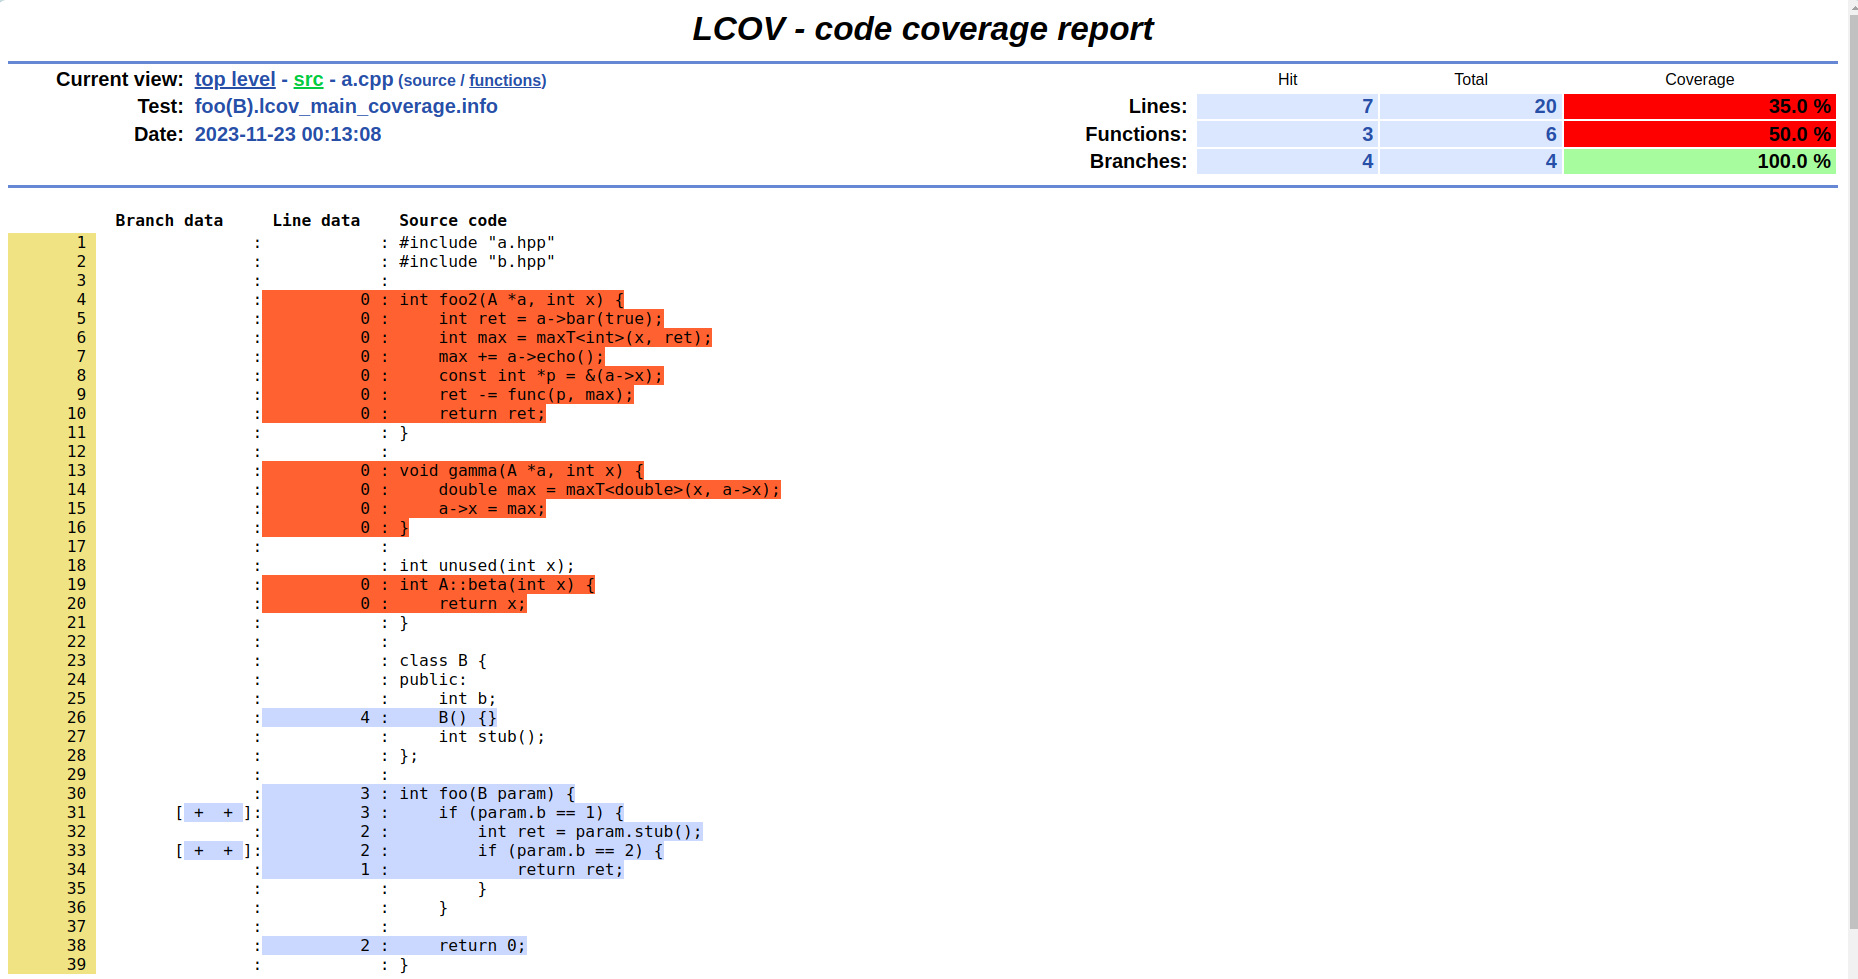
\includegraphics[width=\linewidth]{images/report.png}
    \caption{Báo cáo kiểm thử LCOV của hàm \tcode{foo}.}
    \label{fig:report}
\end{figure}

% \begin{figure}
%     \centering
%     \includesvg[width=0.8\linewidth]{images/module-build.svg}
%     \caption{Các thành phần trong mô-đun xây dựng môi trường kiểm thử.}
%     \label{fig:module-build}
% \end{figure}

% Đầu vào của mô-đun xây dựng môi trường kiểm thử gồm tập mã nguồn kiểm thử và tệp cấu hình kiểm thử được người dùng thiết lập thông qua giao diện của công cụ. Đoạn~mã~\ref{cod:enviro} minh họa tệp cấu hình kiểm thử đầu vào. Dòng 2-11 trong đoạn mã cho biết môi trường kiểm thử sử dụng trình biên dịch GNU mặc định của máy kèm theo một số câu lệnh cơ bản để biên dịch mã nguồn kiểm thử. Dòng 12-14 cho biết thêm thông tin về tên của môi trường kiểm thử, phương pháp kiểm thử cũng như loại độ phủ sẽ được tính là gì. Môi trường ví dụ có tên là \tcode{auto-sample}, sử dụng phương pháp kiểm thử tự động đề xuất bởi khóa luận và hai kiểu độ phủ được tính là độ phủ câu lệnh và độ phủ MCDC. Tệp cấu hình kiểm thử được lưu lại nhằm phục vụ cho các lần kiểm thử sau trên cùng môi trường \tcode{auto-sample}. 
% \begin{figure}[h]
% \begin{lstlisting}[language={}, caption={Tệp cấu hình kiểm thử.}, captionpos=b, label={cod:enviro}]
% ENVIRO.NEW
% ENVIRO.COMPILER.NEW
% ENVIRO.COMPILER.NAME: [GNU Native] C++
% ENVIRO.COMPILER.COMPILE_CMD: g++ -c -w
% ENVIRO.COMPILER.PREPROCESS_CMD: g++ -c -E
% ENVIRO.COMPILER.LINK_CMD: g++ -w
% ENVIRO.COMPILER.INCLUDE_FLAG: -I
% ENVIRO.COMPILER.DEFINE_FLAG: -D
% ENVIRO.COMPILER.OUTPUT_FLAG: -o
% ENVIRO.COMPILER.OUTPUT_EXT: .out
% ENVIRO.COMPILER.END
% ENVIRO.NAME: auto_sample
% ENVIRO.TESTING_METHOD: PROPOSED-METHOD
% ENVIRO.COVERAGE_TYPE: STATEMENT+MCDC
% ENVIRO.END
% \end{lstlisting}
% \end{figure}
\subsection{Mô-đun phân tích mã nguồn}\label{sec:module-analyze}
Mô-đun phân tích mã nguồn đảm nhiệm vai trò trích xuất, phân tích thông tin từ AST của mã nguồn kiểm thử, xây dựng đồ thị cấu trúc mã nguồn và cung cấp dịch vụ tìm kiếm thông tin đỉnh trên đồ thị. Hình~\ref{fig:module-analyze} mô tả cấu trúc của mô-đun với ba thành phần lần lượt là thành phần sinh AST, thành phần sinh đồ thị cấu trúc mã nguồn và thành phần tìm kiếm trên đồ thị. Trong đó, khóa luận kế thừa thành phần sinh AST, cải tiến mô-đun sinh đồ thị cấu trúc mã nguồn và bổ sung thành phần tìm kiếm trên đồ thị.
\vspace{5mm}
\begin{figure}[h]
    \centering
    \includesvg[width=0.8\linewidth]{images/module-analyze.svg}
    \caption{Các thành phần trong mô-đun phân tích mã nguồn.}
    \label{fig:module-analyze}
\end{figure}

Mô-đun phân tích mã nguồn nhận đầu vào là mã nguồn kiểm thử gốc và các đỉnh tệp từ đầu ra của mô-đun xây dựng môi trường. Bắt đầu từ mỗi đỉnh tệp, dựa trên quan hệ cha con trên AST của từng tệp mã nguồn, quá trình sinh cây cấu trúc tệp được diễn ra song song. Sau đó, tập cây cấu trúc tệp được chuyển sang thành phần hoàn thiện đồ thị cấu trúc để bổ sung cạnh kế thừa và cạnh lời gọi hàm. Tại thành phần này, từng cây cấu trúc tệp được xét và tìm kiếm các đỉnh có tiêu chí phù hợp với kiểu cạnh đang xét trên các cây cấu trúc còn lại. Kết quả của quá trình xây dựng là đồ thị cấu trúc mã nguồn kiểm thử.

Khóa luận đã cải tiến thành phần sinh đồ thị cấu trúc mã nguồn như sau. Trước hết, khóa luận tích hợp thành phần ánh xạ cây cấu trúc và thành phần phân tích phụ thuộc~\cite{TUNG2022106821} trong kiến trúc gốc thành mô-đun sinh đồ thị cấu trúc mã nguồn. Quá trình tích hợp bổ sung các luồng xử lý song song quá trình sinh cây cấu trúc tệp giúp giảm thời gian phân tích mã nguồn. Sau đó, khóa luận bổ sung các loại đỉnh mới biểu thị cho các kiểu khai báo mới trong ngôn ngữ C++ như không gian tên, câu lệnh sử dụng không gian tên, khai báo lớp không cần tên kiểu, v.v. Qua đó, thành phần này có thể phân tích và biểu diễn được các đặc trưng mới của C++ trên đồ thị cấu trúc mã nguồn.\\

Tìm kiếm thông tin đỉnh trên đồ thị là quá trình cốt lõi phục vụ cho quá trình xử lý hàm thiếu định nghĩa và quá trình sinh dữ liệu kiểm thử tự động. Trong kiến trúc gốc, quá trình tìm kiếm duyệt qua các đỉnh trên đồ thị, kiểm tra thông tin của đỉnh có hợp với tiêu chí tìm kiếm rồi thêm vào tập kết quả nếu hợp lệ. Trong thực tế, đồ thị cấu trúc thường rất lớn. Vậy nên quá trình tìm kiếm tốn nhiều bộ nhớ bởi quá trình đệ quy xuống đỉnh. Để khắc phục nhược điểm này, khóa luận bổ sung thành phần tìm kiếm trên đồ thị với ý tưởng chính dựa trên tìm kiếm kết hợp bảng băm và cơ sở dữ liệu. Việc tìm kiếm thông tin đỉnh thường sử dụng hai tiêu chí đó là tên hàm và tên kiểu. Tận dụng điều này, khóa luận tạo cơ sở dữ liệu lưu trữ thông tin về kiểu và hàm của mã nguồn kiểm thử. Cơ sở dữ liệu gồm hai trường chính đó là $id$ - khóa chính biểu thị mã định danh của hàm hoặc kiểu và $name$ - tên hàm hoặc tên kiểu. Sau quá trình xây dựng đồ thị cấu trúc mã nguồn, mỗi đỉnh trong đồ thị được cấp một mã định danh cố định $id$. Mã định danh này là giá trị băm xâu đường dẫn của đỉnh, trong đó xâu đường dẫn là chuỗi tên các đỉnh trên đường đi từ đỉnh tệp xuống đỉnh đang xét. Khóa luận sử dụng một bảng băm để ánh xạ $id$ và đỉnh sở hữu $id$. Để nhanh chóng tìm kiếm tên trong cơ sở dữ liệu, khóa luận sử dụng hệ quản trị cơ sở dữ liệu SQLite\footnote{https://www.sqlitetutorial.net/sqlite-full-text-search/} với cơ chế FULLTEXT INDEX trên cột $name$. Để tìm kiếm một đỉnh phù hợp, trước hết quá trình tìm kiếm sẽ thu thập các dòng trong cơ sở dữ liệu có chứa tên hàm hoặc tên kiểu, trích xuất $id$ và dựa vào bảng băm để lấy ra đỉnh cần xét. 

Quá trình nghiên cứu, cải tiến mô-đun phân tích mã nguồn tốn nhiều thời gian do số lượng tệp ảnh hưởng bởi mô-đun này là rất lớn (113 tệp ảnh hưởng và 5476 LOC thay đổi). Tuy nhiên, quá trình trên là cần thiết bởi công cụ AKAUTAUTO phiên bản 5.9.2 thường gặp lỗi hết bộ nhớ ảo trong quá trình phân tích mã nguồn khi chạy trên các dự án có kích thước lớn, cấu trúc phức tạp và có nhiều sự tương tác trong các thành phần với nhau. Sau quá trình cải tiến, công cụ AKAUTAUTO phiên bản 5.9.2-thesis đã có thể phân tích được những bộ mã nguồn có kích thước lớn, đồng thời không gặp tình trạng hết bộ nhớ ảo trong quá trình chạy.

\subsection{Mô-đun xử lý hàm thiếu định nghĩa}\label{sec:module-undef}
Mô-đun xử lý hàm thiếu định nghĩa được khóa luận bổ sung so với kiến trúc gốc nhằm thực hiện nhiệm vụ của pha xử lý hàm thiếu định nghĩa. Hình~\ref{fig:module-undef} mô tả các thành phần cấu thành lên mô-đun gồm thành phần thu thập, thành phần lọc tìm ứng viên, thành phần xử lý nguyên mẫu hàm ảo và thành phần sinh thân hàm giả. Mô-đun xử lý hàm thiếu định nghĩa được thiết kế để xử lý hai loại nguyên mẫu hàm thiếu định nghĩa như đã mô tả ở Mục~\ref{sec:handle-undef}. Chi tiết về các thành phần như sau.
\begin{itemize}
    \item Thành phần thu thập: Đóng vai trò thu thập danh sách các nguyên mẫu hàm thiếu định nghĩa cần sinh thân hàm giả. Thành phần thu thập sử dụng các công cụ tiện ích của trình biên dịch để thu thập danh sách này. Phương pháp thu thập đã được trình bày ở Mục~\ref{sec:handle-undef-first}.
    \item Thành phần xử lý nguyên mẫu hàm ảo: Có chức năng tìm kiếm các nguyên mẫu hàm ảo thiếu định nghĩa sử dụng phương pháp đề xuất ở Mục~\ref{sec:handle-undef-second}. Danh sách các nguyên mẫu hàm ảo tìm được sẽ được truyền sang thành phần lọc tìm ứng viên để xử lý theo Thuật~toán~\ref{alg:handle-virtual-undef}. Các nguyên mẫu hàm ảo còn lại sẽ được sinh cạnh định nghĩa tương ứng với đỉnh biểu thị hàm trong đồ thị cấu trúc.
    \item Thành phần lọc tìm ứng viên: Thực hiện quá trình áp dụng Thuật~toán~\ref{alg:filter-undef} trên danh sách các hàm thiếu định nghĩa trả về bởi thành phần thu thập và các nguyên mẫu hàm ảo thiếu định nghĩa tìm được. Đầu ra của thành phần là danh sách các đỉnh trên đồ thị cấu trúc mã nguồn cần được sinh hàm giả. 
    \item Thành phần sinh thân hàm giả: Đảm nhiệm vai trò sinh thân hàm giả cho danh sách các đỉnh được tổng hợp bởi thành phần lọc tìm ứng viên.
\end{itemize}

\begin{figure}[h]
    \centering
    \includesvg[width=0.8\linewidth]{images/module-undef.svg}
    \caption{Các thành phần trong mô-đun xử lý hàm thiếu định nghĩa.}
    \label{fig:module-undef}
\end{figure}

Đầu ra của mô-đun xử lý hàm thiếu định nghĩa là mã nguồn chứa các câu lệnh đánh dấu đã được bổ sung thân hàm giả cho các nguyên mẫu hàm thiếu định nghĩa. Mã nguồn đã chỉnh sửa này sau đó được sử dụng để tính toán độ phủ khi chạy các ca kiểm thử bởi mô-đun thực thi và phân tích ca kiểm thử.

\subsection{Mô-đun sinh dữ liệu kiểm thử}\label{sec:module-autogen}
Mục tiêu của mô-đun sinh dữ liệu kiểm thử là tự động tạo ra các ca kiểm thử cho các đơn vị cần kiểm thử. Mô-đun được thiết kế như Hình~\ref{fig:module-autogen} với bốn thành phần lần lượt là thành phần sinh CFG, thành phần sinh dữ liệu kiểm thử ngẫu nhiên, thành phần thực thi tượng trưng và thành phần xử lý lời gọi hàm. Trong đó, thành phần xử lý lời gọi hàm được cải tiến bởi phương pháp đề xuất ở Mục \ref{sec:autostub-obj}, các thành phần còn lại được kế thừa từ kiến trúc gốc. Chi tiết về các thành phần như sau.
\begin{itemize}
    \item Thành phần sinh CFG: Có chức năng xây dựng CFG cho các đơn vị trong mã nguồn.
    \item Thành phần sinh dữ liệu kiểm thử ngẫu nhiên: Đảm nhiệm vai trò sinh các ca kiểm thử với dữ liệu ngẫu nhiên trong pha sinh dữ liệu kiểm thử tự động (mô tả ở Mục~\ref{sec:autogen}). 
    \item Thành phần thực thi tượng trưng: Đóng vai trò thực hiện quá trình thực thi tượng trưng trên đường thi hành chưa được viếng thăm và sinh ra các ràng buộc tạo các điểm quyết định trong đồ thị dòng điều khiển. Sau đó, thành phần thực thi tượng trưng sử dụng bộ giải Z3 để giải các ràng buộc và tạo ra các giá trị đầu vào mới.
    \item Thành phần xử lý lời gọi hàm: Có nhiệm vụ tạo giả lập mã nguồn tự động cho các lời gọi hàm xuất hiện trong đường thi hành. Khóa luận kế thừa thành phần xử lý lời gọi hàm dựa trên phương pháp AS4UT và áp dụng phương pháp xử lý lời gọi phương thức được đề xuất ở Mục \ref{sec:autostub-obj}. Đầu ra của thành phần là các thay đổi cần thiết trên CFG, bảng $MAP$ và $REF$ để giúp quá trình thực thi tượng trưng sinh ra bộ dữ liệu kiểm thử mới cho đường thi hành chưa viếng thăm.
\end{itemize}

\begin{figure}[h]
    \centering
    \includesvg[width=0.6\linewidth]{images/module-autogen.svg}
    \caption{Các thành phần trong mô-đun sinh dữ liệu kiểm thử.}
    \label{fig:module-autogen}
\end{figure}
% \subsection{Mô-đun thực thi và phân tích ca kiểm thử}
% \begin{figure}
%     \centering
%     \includesvg[width=0.8\linewidth]{images/module-execute.svg}
%     \caption{Các thành phần trong mô-đun thực thi và phân tích ca kiểm thử.}
%     \label{fig:module-execute}
% \end{figure}

% Đoạn mã \ref{cod:driver} minh họa ví dụ trình điều khiển kiểm thử sinh bởi mô-đun khi kiểm thử hàm \tcode{foo} trong Đoạn~mã~\ref{cod:autostub-object}. Dòng đầu tiên trong trình điều khiển dùng để thiết lập tên đơn vị kiểm thử, giúp các hàm được stub biết cần phải chạy mã nguồn giả lập nào (mô tả trong Đoạn~mã~\ref{cod:stub-final}). Dòng 2-3 định nghĩa tham số đầu vào \tcode{param} của hàm \tcode{foo} là một đối tượng của lớp \tcode{B} với thuộc tính \tcode{b} có giá trị 1. Dòng 4 trong trình điều khiển dùng để gọi hàm \tcode{foo} với các định nghĩa tham số được khai báo ở trên. Kết quả viếng thăm sau quá trình chạy ca kiểm thử được mô tả bởi Đoạn~mã~\ref{cod:visited}. Kết quả viếng thăm cho biết các dòng 8, 9, 10, 11 và nhánh đúng của biểu thức điều kiện ở dòng 8, 10 trong hàm \tcode{foo} được thăm. \\

% \begin{figure}[h]
%     \begin{minipage}[t]{0.5\linewidth}
%     \begin{lstlisting}[language={C++}, caption={Trình điều khiển kiểm thử cho Đoạn mã \ref{cod:autostub-object}.}, captionpos=b, label={cod:driver}]
% TEST_CASE_NAME = "foo";
% B param;
% param.b = 1;
% int AKA_ACTUAL_OUTPUT = foo(param);
%     \end{lstlisting}
%     \end{minipage}
%     \begin{minipage}[t]{0.5\linewidth}
%     \begin{lstlisting}[language=C++, caption={Danh sách các câu lệnh và nhánh điều kiện được thăm bởi trình điều khiển.}, label={cod:visited}, captionpos=b]
% visit_line_8
% visit_condition_1_T
% visit_line_9
% visit_line_10
% visit_condition_1_T
% visit_line_11
%     \end{lstlisting}
% \end{minipage}
% \end{figure}

\section{Mục tiêu, độ đo đánh giá và dữ liệu thực nghiệm}
Mục tiêu tổ chức thực nghiệm là để đánh giá tính hiệu quả của phương pháp đề xuất trên hai tiêu chí với các độ đo tương ứng như sau:
\begin{enumerate}
    \item Đánh giá tính hiệu quả trong quá trình chuẩn bị môi trường kiểm thử cho mã nguồn thiếu định nghĩa giữa phương pháp xử lý hàm thiếu định nghĩa (trình bày ở Mục~\ref{sec:handle-undef}) và phương pháp truyền thống. Để so sánh giữa hai phương pháp, khóa luận sử dụng độ đo thời gian cần thiết để chuẩn bị môi trường kiểm thử. Ngoài ra, khóa luận cũng xem xét tính đúng đắn của phương pháp đề xuất.
    \item Đánh giá tính hiệu quả khi sinh dữ liệu kiểm thử tự động cho một số mã nguồn C/C++ giữa phương pháp đề xuất ở Mục~\ref{sec:autostub-obj} và phương pháp hiện tại trong công cụ phiên bản 5.9.2 - phương pháp kiểm thử tượng trưng động kết hợp tự động giả lập mã nguồn AS4UT (gọi tắt là phương pháp AKAUTAUTO). Để so sánh giữa hai phương pháp, khóa luận sử dụng các độ đo về độ phủ mã nguồn $C_1$, $C_3$, số lượng ca kiểm thử sinh ra, thời gian sinh và bộ nhớ sử dụng trung bình cho mỗi ca kiểm thử.
\end{enumerate}

Về môi trường thực nghiệm, khóa luận sử dụng máy tính với các thông số cấu hình như sau: Ubuntu 22.04, AMD® Ryzen™ 7-5800H CPU @ 3.2GHz x 8, 16GBs RAM. Thực nghiệm được tiến hành trên một số mã nguồn mở trên Github và mã nguồn dự án thực tế thuộc đơn vị FPT-GAM như sau:
\begin{itemize}
    \item C-plus-plus\footnote{https://github.com/TheAlgorithms/C-Plus-Plus} (42179 LOC): Mã nguồn mở viết bằng ngôn ngữ C++ cài đặt các thuật toán thường sử dụng trong lập trình thi đấu và khoa học máy tính.
    \item Box2d\footnote{https://github.com/erincatto/box2d} (78811 LOC): Một thư viện cung cấp các phương thức để tính toán sự tương tác vật lý giữa các vật thể trong môi trường 2 chiều.
    \item FPT1 (23024 LOC): Mô-đun vận hành và điều hướng các yêu cầu gửi đến các dịch vụ trong trình điều khiển đa phương tiện, thuộc một dự án phát triển phần mềm xe ô tô của đơn vị FPT-GAM.
    \item FPT2 (35891 LOC): Mô-đun cung cấp dịch vụ quản lý danh bạ, cuộc gọi trên trình điều khiển đa phương tiện, cũng thuộc dự án trên.
\end{itemize}

Khóa luận sử dụng hai dự án mã nguồn mở nhằm đảm bảo tính khách quan của thực nghiệm. Trong đó, dự án C-plus-plus được sử dụng để đánh giá khả năng sinh dữ liệu kiểm thử của phương pháp đề xuất trên các mã nguồn đơn giản, ít sự liên kết giữa các tệp. Dự án Box2d được chọn để đánh giá tính hiệu quả của phương pháp đề xuất trên các mã nguồn sử dụng nhiều đặc trưng mới của C++. Thêm vào đó, khóa luận cũng sử dụng hai mã nguồn thuộc đơn vị FPT-GAM nhằm đồng thời đánh giá tính hiệu quả và khả năng áp dụng thực tiễn của phương pháp đề xuất.

\section{Đánh giá khả năng xử lý hàm thiếu định nghĩa}
\subsection{Cách thức tổ chức thực nghiệm}
Nhằm đánh giá tính hiệu quả về mặt thời gian khi xử lý hàm thiếu định nghĩa, đồng thời đảm bảo tính khách quan của thực nghiệm, quá trình thực nghiệm được tiến hành bởi lập trình viên\footnote{Trần Trọng Năm - namtt25@fpt.com} trực thuộc đơn vị FPT-GAM. Để mô phỏng môi trường chứa hàm thiếu định nghĩa, khóa luận tiến hành thực nghiệm tính toán thời gian cần thiết để chuẩn bị môi trường kiểm thử cho một số mô-đun trong các mã nguồn mở kể trên. Ba mô-đun thực nghiệm gồm mô-đun collision (xử lý va chạm) trong mã nguồn Box2d, mô-đun FPT1 và mô-đun FPT2. Do mã nguồn C-plus-plus gồm các tệp mã nguồn không liên quan đến nhau nên khóa luận không đánh giá khả năng xử lý hàm thiếu định nghĩa trên mã nguồn này.

Chuẩn bị môi trường kiểm thử là bước đầu tiên trong quy trình kiểm thử tự động. Trong bước này, lập trình viên cần bóc tách mã nguồn mình cần kiểm thử trong dự án và chỉnh sửa mã nguồn sao cho ta có thể tạo được tệp thực thi từ mã nguồn. Để tạo được tệp thực thi, lập trình viên cần xác định các kiểu dữ liệu và các hàm được sử dụng trong mã nguồn mà nằm ở mô-đun khác rồi xử lý các thành phần này để biên dịch được mã nguồn. Sau đó, lập trình viên cần xử lý các hàm thiếu định nghĩa phát sinh do mô-đun chưa phát triển xong để liên kết được các tệp và tạo thành tệp thực thi. Khóa luận tiến hành thu thập thời gian lập trình viên chuẩn bị môi trường kiểm thử giữa phương pháp truyền thống (tức làm thủ công các bước) và phương pháp đề xuất (tức làm thủ công hai bước đầu và để công cụ tự động xử lý các hàm thiếu định nghĩa).
\subsection{Kết quả thực nghiệm}
Bảng~\ref{tab:time_undef} trình bày kết quả thực nghiệm trên mô-đun Box2d, FPT1 và FPT2. Các cột trong bảng có ý nghĩa như sau:
\begin{itemize}
    \item "Module": Tên mô-đun được xét.
    \item "File": Số lượng tệp trong mô-đun.
    \item "Undef": Số lượng hàm thiếu định nghĩa sau khi bóc tách mô-đun.
    \item "Compilable": Thời gian cần thiết để bóc tách mô-đun và chỉnh sửa mã nguồn sao cho biên dịch được.
    \item "Linkable": Thời gian cần thiết để xử lý các hàm thiếu định nghĩa sao cho tạo tệp thực thi được. Trong đó, cột "Manual" thể hiện thời gian xử lý thủ công còn cột "Propose" thể hiện thời gian xử lý sử dụng phương pháp đề xuất (tính bằng giây).
\end{itemize}

\begin{table}[h]
    \centering
    \caption{Kết quả thời gian chuẩn bị môi trường trên ba mô-đun thực nghiệm}
    \label{tab:time_undef}
\begin{tabular}{|l|l|l|l|ll|}
\hline
\multicolumn{1}{|c|}{\multirow{2}{*}{\textbf{Module}}} & \multicolumn{1}{c|}{\multirow{2}{*}{\textbf{File}}} & \multicolumn{1}{c|}{\multirow{2}{*}{\textbf{Undef}}} & \multirow{2}{*}{\textbf{Compilable}} & \multicolumn{2}{c|}{\textbf{Linkable}} \\ \cline{5-6} 
\multicolumn{1}{|c|}{}                                 & \multicolumn{1}{c|}{}                               & \multicolumn{1}{c|}{}                                &                                      & \multicolumn{1}{l|}{Manual}  & Propose \\ \hline
collision (Box2d)                                      & 53                                                  & 5                                                    & 0:02:39                              & \multicolumn{1}{l|}{0:08:23} & 0:00:04 \\ \hline
FPT1                                     & 45                                                  & 263                                                  & 1:04:22                              & \multicolumn{1}{l|}{0:14:48} & 0:00:28 \\ \hline
FPT2                                          & 126                                                 & 333                                                  & 2:05:56                              & \multicolumn{1}{l|}{1:31:01} & 0:02:24 \\ \hline
\end{tabular}
\end{table}

Kết quả thực nghiệm cho thấy thời gian xử lý các hàm thiếu định nghĩa thủ công chiếm một phần đáng kể trong tổng thời gian chuẩn bị môi trường, trong đó thời gian xử lý trên mô-đun collision là 75,98\%, 18,70\% với mô-đun FPT1 và 41,96\% với mô-đun còn lại. Khi áp dụng phương pháp đề xuất, thời gian xử lý các hàm thiếu định nghĩa giảm đáng kể so với phương pháp truyền thống, giảm 8 phút 19 giây trên mô-đun collision, 14 phút 20 giây trên mô-đun FPT1 và giảm 1 tiếng 29 phút trên mô-đun còn lại. Dựa vào kết quả, có thể nhận thấy rằng thời gian xử lý của hai phương pháp phụ thuộc vào số lượng hàm thiếu định nghĩa có trong mô-đun.

\subsection{Đánh giá}
Kết quả thực nghiệm cho thấy rằng phương pháp đề xuất có khả năng giảm đáng kể thời gian chuẩn bị môi trường kiểm thử cho mã nguồn chứa hàm thiếu dịnh nghĩa. Một số lí do chính dẫn đến sự cải thiện đáng kể này như sau:
\begin{itemize}
    \item Trước hết, thời gian xử lý thủ công bị ảnh hưởng bởi kích thước và độ phức tạp của mã nguồn. Các mô-đun có thể phụ thuộc bởi rất nhiều mô-đun khác và đồng thời chúng cũng chứa rất nhiều tệp. Điều này gây khó khăn cho lập trình viên khi họ cần xác định vị trí các tệp chứa hàm thiếu định nghĩa. Phương pháp đề xuất chỉ quan tâm tới danh sách các hàm trả về bởi trình biên dịch và kết hợp duyệt trên đồ thị cấu trúc mã nguồn nên nhanh chóng xác định và xử lý đúng hàm thiếu định nghĩa.
    \item Quá trình xử lý hàm thiếu định nghĩa thủ công đòi hỏi lập trình viên có kiến thức về mã nguồn kiểm thử. Điều này khiến lập trình viên tốn nhiều thời gian để nghiên cứu mã nguồn và xử lý chính xác các hàm thiếu định nghĩa. Trong bối cảnh ngôn ngữ C++ đang được phát triển với nhiều đặc trưng mới ra mắt, việc xử lý thủ công có thể tiêu tốn nhiều chi phí về nhân lực và thời gian hơn.
    \item Cuối cùng, phương pháp đề xuất có thể xử lý song song các hàm trong khi lập trình viên cần xử lý tuần tự từng hàm. Điều này dẫn tới thời gian xử lý giảm đáng kể so với phương pháp truyền thống.
\end{itemize}

Để đánh giá tính đúng đắn của phương pháp đề xuất, khóa luận đã tiến hành thực nghiệm sinh dữ liệu kiểm thử tự động cho các đơn vị trong mã nguồn sau khi xử lý hàm thiếu định nghĩa (trình bày ở Mục~\ref{sec:evaluate-autogen}). Kết quả cho thấy các ca kiểm thử đều thực thi được và không gặp lỗi trong quá trình liên kết. Như vậy, phương pháp đề xuất đã xử lý đúng và đủ các hàm thiếu định nghĩa cần thiết. Điều này được khẳng định bởi nếu phương pháp xử lý thiếu hoặc sai hàm, mã nguồn kiểm thử không thể liên kết và thực thi các ca kiểm thử được. Tính đến thời điểm nghiên cứu của khóa luận, phương pháp đề xuất đã giải quyết được các mã nguồn thực nghiệm chứa các đặc trưng của ngôn ngữ C++ ở nhiều phiên bản, mới nhất là bản C++20. Tuy nhiên trong các phiên bản tương lai, tính đúng đắn của phương pháp đề xuất có thể bị ảnh hưởng.

Như vậy, phương pháp đề xuất có thể áp dụng vào thực tiễn để giúp giảm thời gian kiểm thử đơn vị tự động. Tuy nhiên, có thể nhận thấy rằng thấy phương pháp đề xuất vẫn còn phụ thuộc vào bước bóc tách mã nguồn và xử lý sao cho biên dịch được. Việc phụ thuộc vào các bước thủ công khiến quá trình chuẩn bị môi trường kiểm thử tốn nhiều thời gian, đặc biệt là khi kiểm thử cho mã nguồn kích thước lớn. Một số lí do dẫn đến phương pháp chưa hoàn toàn tự động được như sau:
\begin{itemize}
    \item Quá trình bóc tách mã nguồn yêu cầu công cụ trích xuất được đúng các tệp có liên quan đến mô-đun người dùng mong muốn kiểm thử. Điều này gây khó khăn bởi để trích xuất được chính xác mô-đun, công cụ cần phân tích mã nguồn của cả dự án để biết được các quan hệ giữa mô-đun và các thành phần khác. Việc phân tích mã nguồn dự án tốn nhiều thời gian và có thể cần phân tích nhiều lần do quá trình phát triển song song với quá trình kiểm thử.
    \item Quá trình tự động xử lý các kiểu dữ liệu và các hàm ở mô-đun khác sao cho biên dịch được mã nguồn có thể không chính xác. Khi kiểm thử, ta muốn hạn chế sự tác động đến mã nguồn gốc. Do vậy, các kiểu dữ liệu và hàm ở mô-đun khác thường được sao chép ở một tệp và mô-đun kiểm thử sẽ sử dụng tệp sao chép này. Khi tự động hóa quá trình này, công cụ cần phân tích mã nguồn để biết chính xác nên sao chép kiểu nào, hàm nào và vị trí ở đâu.
\end{itemize}
 
\section{Đánh giá khả năng sinh dữ liệu kiểm thử tự động}\label{sec:evaluate-autogen}
\subsection{Cách thức tổ chức thực nghiệm}
Nhằm đánh giá tính hiệu quả khi sinh dữ liệu kiểm thử tự động, khóa luận tiến hành thực nghiệm trên công cụ AKAUTAUTO phiên bản 5.9.2, được cài đặt phương pháp kiểm thử tượng trưng động AKAUTAUTO và phương pháp AS4UT, và phiên bản 5.9.2-thesis, được cài đặt phương pháp đề xuất. Các mã nguồn được sử dụng trong thực nghiệm này gồm mã nguồn C-plus-plus, mã nguồn Box2d và mã nguồn FPT1. Khóa luận chưa thể đánh giá khả năng sinh dữ liệu kiểm thử tự động trên mã nguồn FPT2 do mã nguồn này được bảo mật bởi đơn vị FPT-GAM.

\subsection{Kết quả thực nghiệm}
Bảng \ref{tab:autogen-result} trình bày kết quả thực nghiệm sinh dữ liệu kiểm thử tự động cho một số tệp trong các mã nguồn C-plus-plus, Box2d và FPT1 giữa phương pháp AKAUTAUTO và phương pháp đề xuất. Trong đó, bốn tệp đầu được lấy từ dự án C-plus-plus, ba tệp tiếp theo được lấy từ dự án Box2d và năm tệp còn lại từ mô-đun FPT1. Các cột trong bảng có ý nghĩa như sau:
\begin{itemize}
    \item "File": Tên tệp mã nguồn đuôi .cpp được kiểm thử.
    \item "Unit": Số lượng hàm trong tệp mã nguồn được kiểm thử.
    \item "C1": Độ phủ $C_1$ của tệp mã nguồn.
    \item "C3": Độ phủ $C_3$ của tệp mã nguồn.
    \item "Num": Số lượng ca kiểm thử cần thiết để đạt được độ phủ tương ứng.
    \item "Mem": Bộ nhớ sử dụng trung bình (KB) khi sinh dữ liệu kiểm thử tự động cho một hàm trong tệp.
    \item "Time": Thời gian sinh trung bình (giây) khi sinh dữ liệu kiểm thử tự động cho một hàm trong tệp.
\end{itemize}

\begin{table}[h]
    \centering
    \caption{Kết quả thực nghiệm sinh dữ liệu kiểm thử tự động cho một số mã nguồn}
    \label{tab:autogen-result}
\resizebox{\textwidth}{!}{%
\begin{tabular}{|l|l|lllll|lllll|}
\hline
\multicolumn{1}{|c|}{\multirow{2}{*}{\textbf{File}}} & \multicolumn{1}{c|}{\multirow{2}{*}{\textbf{Unit}}} & \multicolumn{5}{c|}{\textbf{AKAUTAUTO Current Method}}                                                                                              & \multicolumn{5}{c|}{\textbf{Proposed Method}}                                                                                                                   \\ \cline{3-12} 
\multicolumn{1}{|c|}{}                               & \multicolumn{1}{c|}{}                               & \multicolumn{1}{c|}{C1}    & \multicolumn{1}{c|}{C3}    & \multicolumn{1}{c|}{Num} & \multicolumn{1}{c|}{Mem}     & \multicolumn{1}{c|}{Time} & \multicolumn{1}{c|}{C1}             & \multicolumn{1}{c|}{C3}             & \multicolumn{1}{c|}{Num} & \multicolumn{1}{c|}{Mem}     & \multicolumn{1}{c|}{Time} \\ \hline
avltree.cpp                                          & 10                                                  & \multicolumn{1}{l|}{91}    & \multicolumn{1}{l|}{80.55} & \multicolumn{1}{l|}{38}  & \multicolumn{1}{l|}{1856.31} & 4.42                      & \multicolumn{1}{l|}{\textbf{99.29}} & \multicolumn{1}{l|}{\textbf{100}}   & \multicolumn{1}{l|}{25}  & \multicolumn{1}{l|}{1299.69} & 4.73                      \\ \hline
binary\_search\_tree.cpp                             & 9                                                   & \multicolumn{1}{l|}{100}   & \multicolumn{1}{l|}{100}   & \multicolumn{1}{l|}{24}  & \multicolumn{1}{l|}{1048.37} & 5.61                      & \multicolumn{1}{l|}{\textbf{100}}   & \multicolumn{1}{l|}{\textbf{100}}   & \multicolumn{1}{l|}{42}  & \multicolumn{1}{l|}{870.71}  & 10.90                     \\ \hline
binaryheap.cpp                                       & 11                                                  & \multicolumn{1}{l|}{77.22} & \multicolumn{1}{l|}{24.16} & \multicolumn{1}{l|}{47}  & \multicolumn{1}{l|}{357.88}  & 2.51                      & \multicolumn{1}{l|}{\textbf{94.34}} & \multicolumn{1}{l|}{\textbf{73.75}} & \multicolumn{1}{l|}{46}  & \multicolumn{1}{l|}{238.66}  & 8.32                      \\ \hline
double\_linked\_list.cpp                             & 6                                                   & \multicolumn{1}{l|}{54.44} & \multicolumn{1}{l|}{31.66} & \multicolumn{1}{l|}{15}  & \multicolumn{1}{l|}{3269.37} & 4.43                      & \multicolumn{1}{l|}{\textbf{54.44}} & \multicolumn{1}{l|}{\textbf{31.66}} & \multicolumn{1}{l|}{34}  & \multicolumn{1}{l|}{405.41}  & 14.94                     \\ \hline
b2\_dynamic\_tree.cpp                                & 12                                                  & \multicolumn{1}{l|}{59.06} & \multicolumn{1}{l|}{45.12} & \multicolumn{1}{l|}{56}  & \multicolumn{1}{l|}{1101.79} & 175.82                    & \multicolumn{1}{l|}{\textbf{72.13}} & \multicolumn{1}{l|}{\textbf{64.32}} & \multicolumn{1}{l|}{37}  & \multicolumn{1}{l|}{295.80}  & 102.15                    \\ \hline
b2\_board\_phase.cpp                                 & 7                                                   & \multicolumn{1}{l|}{49.87} & \multicolumn{1}{l|}{26.85} & \multicolumn{1}{l|}{45}  & \multicolumn{1}{l|}{1611.60} & 206.98                    & \multicolumn{1}{l|}{\textbf{83.81}} & \multicolumn{1}{l|}{\textbf{68.75}} & \multicolumn{1}{l|}{31}  & \multicolumn{1}{l|}{5105.65} & 83.35                     \\ \hline
b2\_collide\_edge.cpp                                & 3                                                   & \multicolumn{1}{l|}{51.85} & \multicolumn{1}{l|}{44}    & \multicolumn{1}{l|}{15}  & \multicolumn{1}{l|}{2611.99} & 91.44                     & \multicolumn{1}{l|}{\textbf{76.44}} & \multicolumn{1}{l|}{\textbf{67.13}} & \multicolumn{1}{l|}{32}  & \multicolumn{1}{l|}{6020.06} & 263.73                    \\ \hline
FPT1\_file1.cpp                                    & 185                                                 & \multicolumn{1}{l|}{89.26} & \multicolumn{1}{l|}{60.67} & \multicolumn{1}{l|}{668} & \multicolumn{1}{l|}{442.53}  & 268.36                    & \multicolumn{1}{l|}{\textbf{98.43}} & \multicolumn{1}{l|}{\textbf{96.05}} & \multicolumn{1}{l|}{703} & \multicolumn{1}{l|}{188.49}  & 46.28                     \\ \hline
FPT1\_file2.cpp                               & 17                                                  & \multicolumn{1}{l|}{46.40} & \multicolumn{1}{l|}{29.29} & \multicolumn{1}{l|}{40}  & \multicolumn{1}{l|}{1353.71} & 54.60                     & \multicolumn{1}{l|}{\textbf{95.41}} & \multicolumn{1}{l|}{\textbf{86.55}} & \multicolumn{1}{l|}{75}  & \multicolumn{1}{l|}{23.79}   & 63.33                     \\ \hline
FPT1\_file3.cpp                                   & 1                                                   & \multicolumn{1}{l|}{66.67} & \multicolumn{1}{l|}{16.67} & \multicolumn{1}{l|}{7}   & \multicolumn{1}{l|}{21.34}   & 72.75                     & \multicolumn{1}{l|}{\textbf{100}}   & \multicolumn{1}{l|}{\textbf{100}}   & \multicolumn{1}{l|}{7}   & \multicolumn{1}{l|}{15.20}   & 54.20                     \\ \hline
FPT1\_file4.cpp                                    & 4                                                   & \multicolumn{1}{l|}{63.07} & \multicolumn{1}{l|}{16.67} & \multicolumn{1}{l|}{13}  & \multicolumn{1}{l|}{108.48}  & 278.04                    & \multicolumn{1}{l|}{\textbf{63.07}} & \multicolumn{1}{l|}{\textbf{16.67}} & \multicolumn{1}{l|}{10}  & \multicolumn{1}{l|}{6.68}    & 21.35                     \\ \hline
FPT1\_file5.cpp                                 & 2                                                   & \multicolumn{1}{l|}{92.86} & \multicolumn{1}{l|}{50}    & \multicolumn{1}{l|}{4}   & \multicolumn{1}{l|}{23.34}   & 10.91                     & \multicolumn{1}{l|}{\textbf{92.86}} & \multicolumn{1}{l|}{\textbf{50}}    & \multicolumn{1}{l|}{4}   & \multicolumn{1}{l|}{4.37}    & 9.36                      \\ \hline
\end{tabular}%
}
\end{table}

Kết quả thực nghiệm ở Bảng \ref{tab:autogen-result} cho thấy phương pháp đề xuất sinh dữ liệu kiểm thử có độ phủ $C_1$, $C_3$ luôn cao hơn hoặc bằng phương pháp AKAUTAUTO trên các tệp mã nguồn được kiểm thử. Trong đó, phương pháp đề xuất đạt độ phủ cao hơn khi kiểm thử cho 2/4 tệp của dự án C-plus-plus, 3/3 tệp của dự án Box2d và 3/5 tệp của dự án FPT1. So sánh độ phủ trung bình giữa hai phương pháp trên các tệp của từng dự án, phương pháp đề xuất có độ phủ trung bình cao hơn và tăng đáng kể khi xét độ phủ $C_3$. Cụ thể, với bốn tệp thuộc dự án C-plus-plus, độ phủ $C_1$, $C_3$ trung bình tăng lần lượt 6.35\% và 17.26\%. Ba tệp của dự án Box2d có độ phủ $C_1$, $C_3$ trung bình tăng lần lượt 23.87\% và 28.08\%. Năm tệp của dự án FPT1 tăng lần lượt 18.30\% và 35.19\% với các độ đo tương ứng.

Về mặt độ phủ $C_1$, $C_3$ đạt được trên từng hàm kiểm thử, kết quả trên ba dự án đều cho thấy phương pháp đề xuất đạt được độ phủ cao hơn hoặc bằng phương pháp AKAUTAUTO. Trước hết, với dự án C-plus-plus, các Hình~\ref{fig:c1-algo}, \ref{fig:c3-algo} cho thấy độ phủ $C_1$, $C_3$ của phương pháp đề xuất đạt 100\% cho hầu hết các hàm trong hai tệp đầu, tăng mạnh độ phủ~$C_3$ cho các hàm trong tệp \tcode{binary\_search\_tree.cpp} và giữ nguyên đối với các hàm trong tệp còn lại. Trên dự án Box2d, Hình~\ref{fig:c1-box2d} và \ref{fig:c3-box2d} cho thấy phương pháp đề xuất có tăng đáng kể độ phủ $C_1$, $C_3$ trên 10/22 đơn vị. Tuy nhiên, phương pháp đề xuất không cải thiện độ phủ trên 12 đơn vị còn lại. Cuối cùng, với dự án FPT1, các Hình~\ref{fig:c1-serviceproxy}, \ref{fig:c3-serviceproxy} cho thấy phương pháp đề xuất tăng độ phủ $C_1$, $C_3$ với phần lớn các đơn vị, trong đó 95/209 đơn vị với độ phủ $C_1$ và 173/209 đơn vị với độ phủ $C_3$. Kết quả chi tiết độ phủ trên từng đơn vị kiểm thử cho thấy rằng đối với các đơn vị đã đạt 100\% bởi phương pháp AKAUTAUTO, phương pháp đề xuất cũng đạt 100\% với các đơn vị đó. Tuy nhiên, kết quả độ phủ của phương pháp AKAUTAUTO cho thấy tuy độ phủ $C_1$ của đơn vị có thể đạt 100\% nhưng các nhánh điều kiện trong đơn vị có thể chưa được kiểm tra hết, dẫn tới độ phủ $C_3$ thấp. 

\begin{figure}[H]
    \centering
    \includesvg[width=\linewidth]{images/cppalgo/c1algo.svg}
    \caption{So sánh độ phủ $C_1$ giữa phương pháp đề xuất và phương pháp AKAUTAUTO trên một số hàm trong C-plus-plus.}
    \label{fig:c1-algo}
\end{figure}

\begin{figure}[H]
    \centering
    \includesvg[width=\linewidth]{images/cppalgo/c3algo.svg}
    \caption{So sánh độ phủ $C_3$ giữa phương pháp đề xuất và phương pháp AKAUTAUTO trên một số hàm trong C-plus-plus.}
    \label{fig:c3-algo}
\end{figure}

\begin{figure}[H]
	\centering
	\includesvg[width=\linewidth]{images/box2d/c1box2d.svg}
	\caption{So sánh độ phủ $C_1$ giữa phương pháp đề xuất và phương pháp AKAUTAUTO trên một số hàm trong Box2d.}
	\label{fig:c1-box2d}
\end{figure}

\begin{figure}[H]
	\centering
	\includesvg[width=\linewidth]{images/box2d/c3box2d.svg}
	\caption{So sánh độ phủ $C_3$ giữa phương pháp đề xuất và phương pháp AKAUTAUTO trên một số hàm trong Box2d.}
	\label{fig:c3-box2d}
\end{figure}

\begin{figure}[H]
	\centering
	\includesvg[width=\linewidth]{images/serviceproxy/c1serviceproxy.svg}
	\caption{So sánh độ phủ $C_1$ giữa phương pháp đề xuất và phương pháp AKAUTAUTO trên các hàm trong mô-đun FPT1.}
	\label{fig:c1-serviceproxy}
\end{figure}

\begin{figure}[H]
	\centering
	\includesvg[width=\linewidth]{images/serviceproxy/c3serviceproxy.svg}
	\caption{So sánh độ phủ $C_3$ giữa phương pháp đề xuất và phương pháp AKAUTAUTO trên các hàm trong mô-đun FPT1.}
	\label{fig:c3-serviceproxy}
\end{figure}

Xét số lượng ca kiểm thử tối thiểu sinh để đạt độ phủ tương ứng của hai phương pháp, có thể nhận thấy rằng số ca kiểm thử tối thiểu phụ thuộc vào từng dự án. Đối với dự án C-plus-plus, Hình~\ref{fig:num-algo} cho thấy rằng với các đơn vị không có quá nhiều sự chênh lệnh về độ phủ, số ca kiểm thử tối thiểu chênh lệch ít. Tuy nhiên, với các đơn vị có sự tăng về độ phủ $C_1$ hoặc $C_3$, số ca kiểm thử tăng trong khoảng 2-6 lần. Đặc điểm tương tự diễn ra khi kiểm thử dự án Box2d (mô tả ở Hình~\ref{fig:num-box2d}). Một số trường hợp đột biến về sự chênh lệnh số ca kiểm thử chủ yếu bởi phương pháp xử lý lời gọi phương thức hoặc đơn vị kiểm thử chứa nhiều vòng lặp. Với dự án FPT1, do mã nguồn chứa nhiều sự tương tác giữa các đối tượng, Hình~\ref{fig:num-serviceproxy} cho thấy phần lớn các đơn vị (164/209) có số lượng ca kiểm thử tối thiểu của phương pháp đề xuất nhiều hơn phương pháp AKAUTAUTO.

\begin{figure}[H]
    \centering
    \includesvg[width=\linewidth]{images/cppalgo/numalgo.svg}
    \caption{So sánh số ca kiểm thử sinh ra giữa phương pháp đề xuất và phương pháp AKAUTAUTO trên một số hàm trong C-plus-plus.}
    \label{fig:num-algo}
    
	\includesvg[width=\linewidth]{./images/box2d/numbox2d.svg}
	\caption{So sánh số ca kiểm thử sinh ra giữa phương pháp đề xuất và phương pháp AKAUTAUTO trên một số hàm trong Box2d.}
	\label{fig:num-box2d}

	\includesvg[width=\linewidth]{images/serviceproxy/numserviceproxy.svg}
	\caption{So sánh số ca kiểm thử sinh ra giữa phương pháp đề xuất và phương pháp AKAUTAUTO trên các hàm trong mô-đun FPT1.}
	\label{fig:num-serviceproxy}
\end{figure}

Về thời gian sinh dữ liệu kiểm thử tự động, kết quả cho thấy có 4/4 tệp của dự án C-plus-plus, 1/3 tệp của dự án Box2d và 1/5 tệp của dự án FPT1 mà phương pháp đề xuất sử dụng nhiều thời gian hơn. Ngược lại, phương pháp đề xuất có thời gian sinh ít hơn phương pháp AKAUTAUTO trên các tệp còn lại. Hình~\ref{fig:time-algo}, \ref{fig:time-box2d} và~\ref{fig:time-serviceproxy} phản ánh thời gian sinh dữ liệu kiểm thử cho các tệp trên từng dự án. Do dự án C-plus-plus không chứa nhiều lời gọi phương thức nên phương pháp đề xuất sử dụng nhiều thời gian hơn trên phần lớn các đơn vị kiểm thử. Với hai dự án còn lại, có thể nhận thấy rằng đa phần phương pháp đề xuất sử dụng ít thời gian hơn. Do dự án Box2d chứa nhiều vòng lặp nên thời gian sử dụng phụ thuộc vào số lượng ca kiểm thử và số lần lặp.

\begin{figure}[H]
    \centering
    \includesvg[width=\linewidth]{images/cppalgo/timealgo.svg}
    \caption{So sánh thời gian chạy giữa phương pháp đề xuất và phương pháp AKAUTAUTO trên một số hàm trong C-plus-plus.}
    \label{fig:time-algo}
\end{figure}

\begin{figure}[H]
	\centering
	\includesvg[width=\linewidth]{images/box2d/timebox2d.svg}
	\caption{So sánh thời gian chạy giữa phương pháp đề xuất và phương pháp AKAUTAUTO trên một số hàm trong Box2d.}
	\label{fig:time-box2d}
\end{figure}

\begin{figure}[H]
	\centering
	\includesvg[width=\linewidth]{images/serviceproxy/timeserviceproxy.svg}
	\caption{So sánh thời gian chạy giữa phương pháp đề xuất và phương pháp AKAUTAUTO trên các hàm trong mô-đun FPT1.}
	\label{fig:time-serviceproxy}
\end{figure}

Về bộ nhớ sử dụng để sinh dữ liệu kiểm thử, phương pháp đề xuất sử dụng ít bộ nhớ hơn trên phần lớn các tệp được kiểm thử (10/12). Các trường hợp sử dụng nhiều bộ nhớ hơn là bởi quá trình thực thi tượng trưng xử lý nhiều vòng lặp và các lời gọi phương thức. Ngoài các trường hợp trên, không có lý do rõ ràng giải thích cho sự khác biệt trong lượng bộ nhớ sử dụng của hai phương pháp.

\begin{figure}[H]
    \centering
    \includesvg[width=\linewidth]{images/cppalgo/memalgo.svg}
    \caption{So sánh bộ nhớ sử dụng ra giữa phương pháp đề xuất và phương pháp AKAUTAUTO trên một số hàm trong C-plus-plus.}
    \label{fig:mem-algo}
\end{figure}

\begin{figure}[H]
    \centering
    \includesvg[width=\linewidth]{images/box2d/membox2d.svg}
    \caption{So sánh bộ nhớ sử dụng ra giữa phương pháp đề xuất và phương pháp AKAUTAUTO trên một số hàm trong Box2d.}
    \label{fig:mem-box2d}
\end{figure}

\begin{figure}[H]
    \centering
    \includesvg[width=\linewidth]{images/serviceproxy/memserviceproxy.svg}
    \caption{So sánh bộ nhớ sử dụng giữa phương pháp đề xuất và phương pháp AKAUTAUTO trên các hàm trong mô-đun FPT1.}
    \label{fig:mem-serviceproxy}
\end{figure}

\subsection{Đánh giá}
Kết quả thực nghiệm cho thấy rằng phương pháp đề xuất hiệu quả hơn về mặt độ phủ mã nguồn so với phương pháp AKAUTAUTO khi sinh dữ liệu kiểm thử tự động, đặc biệt ở độ phủ $C_3$. Một số lí do chính dẫn đến sự cải thiện như sau:
\begin{itemize}
    \item Phương pháp đề xuất kế thừa phương pháp kiểm thử tượng trưng động nên có cùng khả năng sinh dữ liệu tự động cho các kiểu dữ liệu nguyên thủy và tự định nghĩa với phương pháp AKAUTAUTO. Bởi vậy, các dự án không chứa nhiều lời gọi phương thức như C-plus-plus vẫn có thể áp dụng phương pháp đề xuất để sinh dữ liệu kiểm thử.
  
    \item Phương pháp đề xuất kế thừa và cải tiến phương pháp AS4UT nên có khả năng giả lập mã nguồn trả về tự động tương tự như AS4UT. Điều này khiến quá trình thực thi tượng trưng xử lý được các ràng buộc liên quan đến giá trị trả về của lời gọi hàm, giúp tăng độ phủ.
    
    \item Độ phủ mã nguồn có sự tăng đột phá bởi cải tiến trong quá trình xử lý lời gọi hàm. Dự án Box2d và FPT1 được viết trên ngôn ngữ C++, sử dụng nhiều đặc trưng hướng đối tượng và các thành phần trong mã nguồn tương tác với nhau thông qua lời gọi phương thức của đối tượng. Do vậy, mã nguồn chứa nhiều biểu thức điều kiện liên quan đến thuộc tính của các đối tượng. Phương pháp đề xuất đã xử lý các lời gọi phương thức nên quá trình thực thi tượng trưng có thể giải được các điều kiện có liên quan đến đối tượng gọi hàm. Phương pháp AS4UT chỉ xử lý cho kết quả trả về của lời gọi hàm nên quá trình thực thi tượng trưng chưa giải được các điều kiện liên quan đến sự thay đổi giá trị của thuộc tính thông qua lời gọi hàm.
\end{itemize}

Tuy nhiên, có thể nhận thấy rằng một số tệp mã nguồn không tăng kết quả độ phủ so với phương pháp AKAUTAUTO. Điều này được lí giải bởi các nguyên nhân sau:
\begin{itemize}
    \item Đơn vị kiểm thử chứa nhiều kiểu dữ liệu chưa được hỗ trợ bởi phương pháp đề xuất như con trỏ thông minh, kiểu dữ liệu template, v.v. Phương pháp đề xuất chưa phân tích được các câu lệnh, điều kiện chứa các kiểu dữ liệu này nên không thể sinh ra các ràng buộc thỏa mãn các câu lệnh, điều kiện tương ứng.
    
    \item Hạn chế trong việc chuyển đổi các câu lệnh, điều kiện trong mã nguồn trong quá trình thực thi tượng trưng khiến phương pháp không tìm được nghiệm khả thi.
    
    \item Đơn vị kiểm thử không chứa lời gọi phương thức nên phương pháp đề xuất không cải thiện được độ phủ. Đóng góp chính của phương pháp đề xuất trong việc sinh dữ liệu kiểm thử tự động nằm ở việc xử lý các lời gọi phương thức. Vì vậy, đối với các đơn vị không chứa lời gọi phương thức, phương pháp đề xuất sẽ cho ra kết quả giống với phương pháp AKAUTAUTO áp dụng AS4UT.
    
    \item Phương pháp đề xuất chưa xử lý tốt vòng lặp xuất hiện trong đơn vị kiểm thử. Các dự án C++ thường chứa nhiều câu lệnh duyệt phần tử trong các tập hợp như \tcode{vector, set}. Các ràng buộc liên quan đến phép duyệt như vậy chưa được hỗ trợ.
    
    \item Phương pháp đề xuất chưa xử lý được lời gọi hàm trong thư viện khiến quá trình thực thi tượng trưng không giải được ràng buộc liên quan đến kết quả của lời gọi thư viện.
\end{itemize}

Về khía cạnh số lượng ca kiểm thử, phương pháp đề xuất sinh nhiều ca kiểm thử hơn nếu mã nguồn chứa lời gọi phương thức. Nguyên nhân là do phương pháp đề xuất cần sinh thêm ca kiểm thử để phủ được điều kiện nhánh liên quan đến sự thay đổi của đối tượng sau lời gọi phương thức.

Hai khía cạnh cuối cùng mà khóa luận đánh giá đó là thời gian và bộ nhớ sử dụng để sinh dữ liệu kiểm thử. Hai yếu tố này phụ thuộc nhiều vào cấu trúc và độ phức tạp của mã nguồn. Trong đó, thời gian xử lý bị ảnh hưởng bởi quá trình thực thi tượng trưng, tìm kiếm kiểu dữ liệu hợp lý và quá trình sinh bộ tham số đầu vào cho đơn vị kiểm thử. Với các dự án sử dụng nhiều lời gọi phương thức, phương pháp đề xuất sử dụng ít thời gian hơn. Nguyên nhân là bởi phương pháp không mất quá nhiều thời gian để giải một đường đi thi hành chứa lời gọi phương thức. Phương pháp AKAUTAUTO cố gắng tìm nghiệm cho các đường thi hành như vậy nên tiêu thụ nhiều thời gian hơn. Khía cạnh bộ nhớ sử dụng cũng ảnh hưởng bởi các yếu tố tương tự. Tuy nhiên, từ kết quả thực nghiệm, có thể nhận thấy rằng phương pháp đã giải quyết được vấn đề liên quan đến lời gọi phương thức và thể hiện tính khả thi khi áp dụng thực tiễn.

\chapter*{Kết luận}\label{chap5}
\addcontentsline{toc}{chapter}{Kết luận}
Khóa luận này đã trình bày chi tiết về quá trình nghiên cứu, thiết kế, và triển khai một hệ thống quản lý nhà hàng toàn diện, đáp ứng nhu cầu của cả chủ nhà hàng và khách hàng.
Hệ thống không chỉ cung cấp các công cụ quản lý hiệu quả cho nhà hàng, quán ăn mà còn tạo ra một nền tảng tương tác thuận tiện cho khách hàng thông qua các tính năng đặt bàn trực tuyến và đặt món trực tuyến thông qua quét mã QR và quản lý thông tin cá nhân.

Việc áp dụng kiến trúc vi dịch vụ cùng với việc tận dụng khả năng mở rộng tự động của GKE đã giúp hệ thống đạt được tính linh hoạt, khả năng chịu lỗi cao và khả năng đáp ứng nhu cầu sử dụng biến động. Các bộ kiểm thử đã chứng minh hiệu quả hoạt động của hệ thống trong việc tự động mở rộng và duy trì tính sẵn sàng cao, đảm bảo trải nghiệm người dùng mượt mà và không bị gián đoạn.

Tuy còn một vài hạn chế trong thiết kế và tích hợp hoàn chỉnh các luồng nghiệp vụ của hệ thống, sau khi các vấn đề được khắc phục trong tương lai gần, hệ thống sẽ tiếp tục được mở rộng và phát triển với các tính năng mới nhằm nâng cao trải nghiệm người dùng và đáp ứng tốt hơn nhu cầu thị trường.
Một số các chức năng trong số đó ao gồm tính năng đặt món trực tuyến trên trang giới thiệu của nhà hàng, quán ăn, quản lý chế độ dinh dưỡng của người dùng, gợi ý món ăn tại trang đặt món, phát triển ứng dụng di động, v.v.

Bên cạnh đó, ứng dụng hoàn toàn có tiềm năng tận dụng những dữ liệu từ cửa hàng cũng như là khách hàng sử dụng nền tảng để áp dụng công nghệ trí tuệ nhân tạo (AI) nhằm phát triển các chức năng đột phá mới.
Ví dụ, AI có thể được sử dụng để phân tích dữ liệu của người dùng, từ đó đưa ra các gợi ý món ăn tùy biến theo các thông tin thu thập được.
Hoặc AI giúp dự đoán xu hướng ẩm thực và hỗ trợ nhà hàng trong việc xây dựng chiến lược kinh doanh hiệu quả.

Với những định hướng phát triển này, hệ thống quản lý nhà hàng được kỳ vọng sẽ đóng góp tích cực vào sự phát triển của ngành dịch vụ ăn uống tại Việt Nam, giúp các nhà hàng tối ưu hóa quy trình quản lý, nâng cao chất lượng dịch vụ và tăng cường khả năng cạnh tranh trên thị trường.
Với sự phát triển không ngừng của công nghệ, hệ thống này sẽ tiếp tục được cải tiến và hoàn thiện, mang đến những giải pháp tiên tiến và hiệu quả hơn cho ngành công nghiệp này.

\chapter{Tài liệu tham khảo}
\printbibliography[keyword={vietnam}, heading=subbibliography, title={Tiếng Việt}, resetnumbers=true]
\printbibliography[notkeyword={vietnam}, heading=subbibliography, title=Tiếng Anh]
\end{document}